\documentclass[a4paper,onecolumn,11pt,unpublished]{quantumarticle}
\pdfoutput=1
\usepackage[T1]{fontenc}
\usepackage[utf8]{inputenc}
\usepackage{amsmath,amssymb,amsthm,mathtools}
\usepackage{booktabs,array,microtype,tikz}
\usepackage[numbers,sort&compress]{natbib}
\usepackage{hyperref}

\hypersetup{
  pdftitle={Explicit graphs with quantum chromatic number three and large chromatic number},
  pdfauthor={Julius A. Zeiss}
}

\newtheorem{theorem}{Theorem}[section]
\newtheorem{lemma}[theorem]{Lemma}
\newtheorem{proposition}[theorem]{Proposition}
\newtheorem{corollary}[theorem]{Corollary}
\theoremstyle{definition}
\newtheorem{definition}[theorem]{Definition}
\newtheorem{remark}[theorem]{Remark}
\newtheorem{problem}{Problem}[section]

\newcommand{\C}{\mathbb C}
\newcommand{\R}{\mathbb R}
\newcommand{\Ftwo}{\mathbb F_2}
\newcommand{\cq}{\chi_{\mathrm q}}
\newcommand{\B}{\operatorname{Box}}
\newcommand{\qto}{\xrightarrow{\mathrm q}}
\newcommand{\col}[1]{\mathtt{#1}}
\DeclareMathOperator{\dist}{dist}
\DeclareMathOperator{\rank}{rank}

\allowdisplaybreaks[2]
\setlength{\emergencystretch}{2em}

\title{Explicit graphs with quantum chromatic number three and large chromatic number}
\author{Julius A. Zeiss}
\email{jzeiss@physik.rwth-aachen.de}
\affiliation{Institute for Quantum Information, RWTH Aachen University, Otto-Blumenthal-Stra\ss e 20, 52074 Aachen, Germany}

\begin{document}
\maketitle

\begin{abstract}
Ciardo and Mottet proved that graphs with quantum chromatic number three can have arbitrarily large classical chromatic number even under $R$-compatible strategies, where measurements within distance $R$ commute. Their construction relies on seven hardness-of-approximation reductions, leading them to ask for explicit families and a direct proof. We provide both by iterating a single graph operation built from the Mermin--Peres square on the triangle. For every level $j\ge1$ and compatibility parameter $R\ge1$, both the $j$th iterate and an explicit sparse induced subgraph have quantum chromatic number three and a box-complex-certified classical chromatic number at least $2j+3$. At fixed $j$ the sparse graph's size grows polynomially in $R$, and at fixed $R$ it grows singly exponentially in $j$. These graphs admit an $R$-compatible strategy of local dimension $4^j$ using adaptive Pauli measurements on $2j$ EPR pairs, and both resources are rigid: \emph{every} quantum $3$-coloring of these graphs has local dimension divisible by $4^j$ and compatibility radius at most $\max\{R,2\}$. Over all graphs with an $R$-compatible quantum $3$-coloring, our sparse family achieves the optimal polynomial scaling in $R$ at fixed classical chromatic number; as that number grows, any box-complex lower bound forces exponentially many edges. We further prove that any graph admitting a quantum $3$-coloring in local dimension three is classically $5$-colorable---attained explicitly at every compatibility radius from Peres' rays---while quantum $3$-colorings in local dimension four force classical $6$-colorability, and those in higher local dimensions imply a tighter exponential upper bound on the classical chromatic number. Finally, we exhibit the smallest known witnesses on $22$ and $165$ vertices for four and five classical colors, lift Lalonde's computer-assisted $15$-vertex lower bound to $21$ vertices for five colors, and extend the construction to every nonbipartite target graph.
\end{abstract}

\section{Introduction}\label{sec:introduction}

In the coloring game for a finite simple graph $G$, two players who cannot communicate each receive a vertex and answer with a color. They must answer with the same color if they receive the same vertex, and with different colors if they receive adjacent vertices. To win with certainty, classical players need $\chi(G)$ colors. Players who share an entangled state need $\cq(G)$ colors, the \emph{quantum chromatic number} of $G$~\cite{GW,CMNSW}.

A \emph{quantum $c$-coloring} of $G$ in \emph{local dimension} $d$ assigns to each vertex $v$ a projective measurement $(P_{v,a})_{a=1}^c$ on $\C^d$, in which some projectors may be zero. It must obey the \emph{edge rule}: $P_{u,a}P_{v,a}=0$ for every edge $uv$ and every color $a$. This characterizes the perfect strategies on a maximally entangled state of local dimension $d$~\cite[Corollary~2.2]{MR}.

Following Ciardo~\cite[Section~3]{C26} and Ciardo and Mottet~\cite[Section~4.1]{CM}, a quantum coloring is \emph{$R$-compatible} if $[P_{u,a},P_{v,b}]=0$ for all colors $a,b$ whenever $\dist_G(u,v)\le R$. The largest such $R$ is its \emph{compatibility radius}. Three colors force $1$-compatibility~\cite[Lemma~2]{Ji}. Compatibility is a locality condition. On every set of vertices of diameter at most $R$, the measurements of an $R$-compatible coloring commute, so they can be performed jointly, and the strategy reduces to a probability distribution over proper classical colorings of that set (Section~\ref{sec:compatibility}). The larger $R$ is, the more global the quantum advantage must be.

Ciardo~\cite[Conjecture~2 and Theorem~7]{C26} showed that graphs with $\cq=3$ and arbitrarily large chromatic number exist if a pseudo-telepathic version of Khot's $d$-to-$1$ conjecture holds for some $d\ge2$. That conjecture asks, for every $\varepsilon>0$ and every $k$, for a $d$-to-$1$ label cover instance of classical value below $\varepsilon$ that has a perfect $k$-compatible quantum assignment. Ciardo and Mottet~\cite[Theorem~1.3]{CM} proved it for every $d\ge4$, building on the reduction to $4$-to-$1$ label cover of Fei, Minzer, and Wang~\cite{FMW}. Consequently, for all $t$ and $R$ there are graphs with $\chi\ge t$ that have an $R$-compatible quantum $3$-coloring~\cite[Theorem~1.4 and Remark~2.5]{CM}. These graphs arise from the Mermin--Peres square through seven reductions from the theory of hardness of approximation, which we list in Section~\ref{sec:comparison}. They are not described explicitly, and both the graphs and the local dimensions are enormous. Ciardo and Mottet expect that a direct proof exists, and they pose the problem of ``finding families of small or explicit graphs witnessing the unbounded $\cq$ vs.\ $\chi$ gap''~\cite[Section~3]{CM}.

We solve this problem with a single graph operation, the \emph{square substitution} $S_\lambda$ (Section~\ref{sec:substitution}), applied repeatedly to the triangle $K_3$. A vertex of $S_\lambda(H)$ prescribes a measurement of two qubits in one of six bases taken from the Mermin--Peres square, followed by the measurement that one of four vertices of $H$ prescribes. The integer $\lambda\ge0$ sets the distance up to which these measurements commute.

\begin{theorem}\label{thm:main}
Let $j,R\ge1$ and $\lambda=\max\{R-2,0\}$, and let $G=S^j_\lambda(K_3)$ be the $j$th iterate of the square substitution on the triangle. Then $\cq(G)=3$ and $\chi(G)\ge2j+3$. Moreover:
\begin{enumerate}
\setlength{\itemsep}{3pt}\setlength{\topsep}{4pt}\setlength{\parsep}{0pt}
\item[\textup{(i)}] $G$ has an explicit $R$-compatible quantum $3$-coloring in local dimension $4^j$, by adaptive Pauli measurements on $2j$ EPR pairs;
\item[\textup{(ii)}] every quantum $3$-coloring of $G$, with no compatibility assumed beyond the edge rule, has local dimension divisible by $4^j$;
\item[\textup{(iii)}] none is $k$-compatible for any $k>\max\{R,2\}$;
\item[\textup{(iv)}] all of this holds for an explicit induced subgraph $G_{j,R}$ of $G$ with $|V(G_{j,R})|+|E(G_{j,R})|\le[C(1+R)]^j$, where $C$ is an absolute constant.
\end{enumerate}
\end{theorem}

Theorem~\ref{thm:main} is assembled in Section~\ref{sec:largest-radius} from Theorems~\ref{thm:gap}, \ref{thm:sparse}, \ref{thm:dimension} and Proposition~\ref{prop:largest-compatible-radius}. Write $N_3(t,R)$ and $D_3(t,R)$ for the minimum order and local dimension over \emph{all} graphs with $\chi\ge t$ and \emph{all} $R$-compatible quantum $3$-colorings. Table~\ref{tab:costs} contrasts these universal bounds with our strategies ($j=\lceil(t-3)/2\rceil$ in $G_{j,R}$), separating fixed-$t$ from fixed-$R$.

\begin{table}[!htbp]
\centering
\footnotesize
\setlength{\tabcolsep}{2.5pt}
\begin{tabular}{@{}llll@{}}
\toprule
Cost of $\chi\ge t$ at $\cq=3$ & Every graph needs & Constructed graphs give & Reference \\
\midrule
Order, fixed $t\ge4$, $R\to\infty$ & $\Omega_t(R^{\lceil(t-3)/2\rceil})$ & $O_t(R^{\lceil(t-3)/2\rceil})$ & Cor.~\ref{cor:radius} \\
Order, fixed $R=1$, $t\to\infty$ & $t^{3+\sqrt6-o(1)}$ & $\exp(O(t))$ & Prop.~\ref{prop:unrestricted-order}, Thm.~\ref{thm:sparse} \\
Edges, box-complex certified & $(2/\sqrt3)^{t-2}$ & $\exp(O(t))$ & Prop.~\ref{prop:box-barrier}, Thm.~\ref{thm:sparse} \\
Local dim., $t\to\infty$ & $(12.23\ldots-o(1))\log_2 t$ & $4^{\lceil(t-3)/2\rceil}$ & Thm.~\ref{thm:rank-rounding}, \eqref{eq:dimension-lower}, Thm.~\ref{thm:sparse} \\
Local dim., $t=4,5$ & $3$ & $3$ & Thm.~\ref{thm:qutrit} \\
Vertices, $t=4$ and $5$ ($R=1$) & $15$ and $21$ \emph{(via~\cite{La})} & $22$ and $165$ & Props.~\ref{prop:order-lower}, \ref{prop:twentytwo}; Thm.~\ref{thm:finite-square} \\
\bottomrule
\end{tabular}
\caption{The cost of chromatic number at least $t$ at quantum chromatic number three: lower bounds that hold for every graph, and the values attained by the graphs of this paper ($G_{j,R}$ of Theorem~\ref{thm:main}, and $Q_R$, $F_{22}$, $F_{\rm phys}$ of Sections~\ref{sec:universal} and~\ref{sec:finite}). The bound in the third row holds for every graph $G$ whose box complex $\B(G)$ admits no equivariant map to the sphere $S^{t-3}$, which is the obstruction behind the lower bounds on $\chi$ in Sections~\ref{sec:iteration} and~\ref{sec:targets}. In the last row, the numbers $15$ and $21$ depend on the computer-assisted classification of Lalonde~\cite{La}.}
\label{tab:costs}
\end{table}

\paragraph{The construction.}
The Mermin--Peres square is a $3\times3$ array of two-qubit Pauli observables in which the three observables of each row and of each column commute. Each row and each column therefore has a common eigenbasis of $\C^4$, which gives six bases. A row and a column have exactly one observable in common, so their two bases share its two eigenspaces, a decomposition of $\C^4$ into two planes. The product of the three observables is $+I$ in every row and in two of the columns, and $-I$ in the third column. Because of this sign, no assignment of values $\pm1$ to the nine observables respects all six products (Lemma~\ref{lem:parity}). The lower bound on the chromatic number, the bound on the local dimension and the bound on the compatibility radius all come from this sign.

A vertex of $S_\lambda(H)$ is an instruction for a measurement: measure two fresh qubits in one of the six bases and, according to which of the four basis vectors is obtained, continue as at the vertex $g_0$, $g_1$, $g_2$ or $g_3$ of $H$. The four vertices form the \emph{word} $g_0g_1g_2g_3$ of the instruction, and only words that repeat their first letter are used. Two instructions with the same basis are adjacent if $g_s$ and $g'_s$ are adjacent in $H$ for all four~$s$. Instructions in a row basis and in a column basis are related only if both depend on nothing but the observable that the two bases share; they are then connected through a \emph{wire} of $\lambda$ intermediate layers of instructions that measure only this observable. A quantum $3$-coloring of $H$ gives one of $S_\lambda(H)$ by carrying out the instruction. The local dimension is multiplied by four, and the measurements along a path with at most $\lambda+2$ edges are diagonal in one of the six bases, so that $R$-compatibility is preserved for $R\le\lambda+2$ (Lemma~\ref{lem:radius-lift}). Substituting $j$ times, starting from the triangle, gives $G$. Its order is doubly exponential in $j$; the subgraph $G_{j,R}$ keeps the vertices whose nested instructions form a tree of bounded size, which makes the order singly exponential and loses none of the properties (Theorem~\ref{thm:sparse}).

\paragraph{Why the chromatic number grows.}
For one substitution on the triangle the lower bound is elementary. A proper $4$-coloring of $S_\lambda(K_3)$ singles out one of the four basis vectors in each basis (Lemma~\ref{lem:four-colorings}), and along each wire the vectors singled out at its two ends lie in the same one of the two shared planes. This would assign consistent values to the nine observables, so no such coloring exists and $\chi(S_\lambda(K_3))=5$ (Theorem~\ref{thm:one-level}). For $j$ substitutions we use the box complex of a graph, a space with a free involution, and the first Stiefel--Whitney class $w$ of that involution: if $w^k\ne0$, the graph needs at least $k+2$ colors (Section~\ref{sec:box}). The box complex of the triangle is a circle, on which $w\ne0$, and we show that the exponent $k$ for which $w^k\ne0$ can be certified grows by two with every substitution (Theorem~\ref{thm:step}). The proof is again a count modulo two. In a space that models the substitution, the loop traced by rotating all four entries of a constant word is, up to boundaries, a sum of other loops in nineteen ways: eighteen, one for each pair of a basis and one of its three observables, and one more that the sign $-I$ forces. When the nineteen sums are added, the other loops cancel in pairs, and since nineteen is odd, the original loop is a boundary. Fillings of this kind are what the powers of $w$ detect (Section~\ref{sec:towers}).

\paragraph{Why no quantum coloring does better.}
In the other direction we start from an arbitrary quantum $3$-coloring of $G_{j,R}$ and use only the edge rule. Its measurements on suitable copies of powers of the triangle inside the graph determine nine involutions in a $3\times3$ array in which the entries of each row and of each column commute, with product $+I$ in every row and in two of the columns and $-I$ in the third column: the relations of the square. Such involutions divide the space into four parts of equal dimension, and repeating the argument inside one of the parts, once for each of the $j$ levels, gives $4^j\mid d$ (Theorem~\ref{thm:dimension}). Two of the nine involutions anticommute, and they are determined by the measurements at four vertices that are pairwise at distance at most $\lambda+3$. Hence no quantum $3$-coloring of the graph is $(\lambda+3)$-compatible (Proposition~\ref{prop:largest-compatible-radius}).

\subsection{Comparison with Ciardo and Ciardo--Mottet}\label{sec:comparison}

Ciardo and Mottet~\cite[Table~1 and Section~3]{CM} obtain their graphs by composing seven reductions that start from the Mermin--Peres square. Each reduction is classically sound and quantum complete:
\begin{list}{}{\setlength{\labelwidth}{3.6em}\setlength{\labelsep}{0.6em}\setlength{\leftmargin}{4.8em}\setlength{\itemsep}{2pt}\setlength{\parsep}{0pt}\setlength{\topsep}{4pt}}
\item[\textup{(i)}] stretching the square by wires of $2m$ auxiliary equations, which gives a label cover with a $(4m+1)$-compatible perfect quantum assignment;
\item[\textup{(ii)}] parallel repetition, which drives the classical soundness to zero;
\item[\textup{(iii)}] multilayered Kneser hypergraphs;
\item[\textup{(iv)}] the reduction of Fei, Minzer, and Wang to $4$-to-$1$ label cover~\cite{FMW};
\item[\textup{(v)--(vi)}] the reductions of Dinur, Mossel, and Regev and of Guruswami and Sandeep~\cite{DMR,GS}, analyzed for quantum strategies in~\cite[Sections~5.1--5.2]{C26}, which produce a graph with a larger quantum palette $2d$;
\item[\textup{(vii)}] iterated line digraphs~\cite[Sections~5.3--5.4]{C26}, which bring the quantum palette back down to $3$ and roughly halve the compatibility in each iteration.
\end{list}
Their Remark~2.6 gives local dimension $4^{n(\ell-1)t\kappa}$ in terms of the reduction parameters, without explicit bounds on graph order.

Our construction shares two core ingredients with~\cite{C26,CM}:
\begin{itemize}
\item \emph{Wire stretching} (credited to Ciardo and Mottet~\cite[Section~2.2 and Proposition~2.1]{CM}): splitting each variable of the square into row and column copies joined by a wire of auxiliary constraints measured with the same binary observable controls compatibility by wire length.
\item \emph{Words evaluated at a measured label} (from the reduction of~\cite{DMR,GS}, whose quantum completeness is proved in~\cite[Section~5.2, Theorem~27, and Proposition~28]{C26}): a level-one vertex pairs a basis with a word assigning a color to each of its four positions.
\end{itemize}
Three structural differences eliminate the hardness-of-approximation chain:
\begin{enumerate}
\item \emph{Adaptive graph recursion instead of parallel repetition:} at level $j$, each letter of a word is a vertex of level $j-1$, and the player measures only the single selected letter on the next register rather than answering every coordinate in parallel.
\item \emph{Fixed palette of three colors:} the quantum palette stays $3$ at every level and the local dimension is multiplied by exactly $4$ per level, so that larger palettes and line digraphs are not needed.
\item \emph{Topological soundness:} the classical lower bound $\chi\ge2j+3$ comes directly from the Stiefel--Whitney height of the box complex raised by two per level by the sign $-I$ of the square, fulfilling Ciardo and Mottet's expectation of a direct proof without complexity-theoretic reductions~\cite[Section~3]{CM}.
\end{enumerate}

\subsection{Related work}\label{sec:related}

When the quantum chromatic number is allowed to grow, Hadamard graphs have long been known to give an exponential separation between $\chi$ and $\cq$~\cite{BCT,AHKS,FR}. For fixed $\cq=3$, early examples separated $\chi=4$ from $\cq=3$ using a reduction from $3$-satisfiability to $3$-coloring~\cite{FILG}. Applying that reduction to the Mermin--Peres square yields the $57$-vertex graph $G_{\rm msg}$ of Man{\v c}inska and Roberson~\cite[Theorem~2; Fact~4 in arXiv~v1]{MR2}, which has $\cq=3$ and $\chi=4$. Lalonde~\cite[Theorem~1.1 of the arXiv version]{La} showed by a computer-assisted classification that every graph with $\cq=3<\chi$ has at least $15$ vertices. That paper also notes $G_{\rm msg}$ as the only reasonably small graph previously reported to separate $\cq$ from its rank-one version, and remarks without proof that graphs from that $3$-SAT reduction are $4$-colorable. In Section~\ref{sec:finite} we exhibit the smallest known explicit witnesses for these first two gaps: the $22$-vertex graph $F_{22}$ with $(\cq,\chi)=(3,4)$ and the $165$-vertex graph $F_{\rm phys}$ with $(\cq,\chi)=(3,5)$. We also lift Lalonde's bound to a new lower bound $|V(G)|\ge21$ for graphs with a quantum $3$-coloring and $\chi\ge5$.

Regarding local dimension, Ciardo~\cite[Corollary~35 and Example~36]{Ciardo24} proved existentially that graphs admitting a quantum $n$-coloring in local dimension three can require $\chi\ge2n-1$ classical colors, in particular $\chi\ge5$ at $\cq=3$. Banakh, Ciardo, Kozik, and Tu{\l}owiecki~\cite[Theorem~29]{BCKT} proved the general upper bound $\chi(G)\le3(2+o(1))^{d-1}$ for every graph $G$ admitting a quantum $3$-coloring in local dimension $d$. Section~\ref{sec:universal} provides explicit graphs $Q_R$ with quantum $3$-colorings in local dimension three and $\chi=5$ at every compatibility radius, and proves that a graph with a quantum $3$-coloring in local dimension three never needs more than five classical colors. It also lowers the base of the general exponential bound from $2$ to $2^{5/3}/3\approx1.0583$.

Topological lower bounds on chromatic numbers originate with Lov{\'a}sz's proof of Kneser's conjecture~\cite{Lov78}. They were developed in equivariant form, for box complexes and Hom complexes, by Matou{\v s}ek~\cite{Mat}, Matou{\v s}ek and Ziegler~\cite{MZ}, Csorba~\cite{Csorba}, and Kozlov~\cite{Kozlov}; we use them through Stiefel--Whitney classes~\cite{MS}. Finally, the algebraic backbone of our construction is the Mermin--Peres square~\cite{Mermin,Peres,KS}, whose intersection graph is $K_{3,3}$~\cite[Example~20]{Arkhipov}; nonplanarity of the intersection graph is Arkhipov's criterion for an arrangement of observables to exhibit parity pseudo-telepathy~\cite[Theorem~21]{Arkhipov}. Our local-dimension rigidity (Theorem~\ref{thm:dimension}) parallels the self-testing of two EPR pairs by the magic square game~\cite{WBMS,CS}. Our cancellation of loops modulo $2$ is close in spirit to topological formulations of parity contextuality~\cite{ORBR}; here it operates inside the box complex and bounds classical colorings.

\subsection{Organization and conventions}\label{sec:organization}

The paper is organized as follows.
\begin{itemize}
\item Section~\ref{sec:construction} treats one substitution. It introduces the six bases of the Mermin--Peres square, works through $S_0(K_3)$ and one vertex of level two, defines $S_\lambda(H)$ with its quantum coloring, and shows that this coloring keeps its compatibility. It then proves $\chi(S_\lambda(K_3))=5$ without topology and extends the construction to arbitrary triads of projections, which gives the graphs $W_\lambda(\mathcal D)$.
\item Section~\ref{sec:iteration} defines the full iterates $S^j_\lambda(K_3)$ and the sparse family $G_{j,R}$, introduces box complexes and towers, proves the lower bound $2j+3$ and the bound on the size, and bounds $\chi(G_{j,R})$ from above.
\item Section~\ref{sec:rigidity} proves that neither the local dimension nor the compatibility radius can be improved on $G_{j,R}$ and $S^j_\lambda(K_3)$, and it completes the proof of Theorem~\ref{thm:main}.
\item Section~\ref{sec:universal} proves the trade-offs between order, compatibility radius, and local dimension that hold for all graphs. They are the first five rows of Table~\ref{tab:costs}.
\item Section~\ref{sec:finite} presents the graphs $F_{22}$ and $F_{\rm phys}$, determines which of them can start the iteration, and derives the lower bound $21$ on the order from Lalonde's bound $15$ (the last row of Table~\ref{tab:costs}).
\item Section~\ref{sec:targets} extends the construction to every nonbipartite target graph.
\item Section~\ref{sec:discussion} collects all graphs constructed in the paper in Table~\ref{tab:graphs} and lists open problems.
\end{itemize}
Technical proofs are placed in Appendices~\ref{app:four}--\ref{app:readings}.

\emph{Conventions.} The projectors of a quantum coloring are always written $P_{v,a}$, with a vertex and a color as indices. The symbols $P_e$ and $P^i_r$ denote the fixed projections of the Mermin--Peres square that are introduced in Section~\ref{sec:square}. The colors of a quantum $c$-coloring are $1,\ldots,c$. For three colors we regard them as the elements of $\mathbb Z/3$, so that $0$ and $3$ denote the same color; depending on the section, they are written $0,1,2$ or $1,2,3$. Every graph with a quantum $2$-coloring is bipartite~\cite[Proposition~3]{CMNSW}. Hence a graph that contains a triangle and has a quantum $3$-coloring has quantum chromatic number exactly three; we use this fact without further reference.

\section{One level: the Mermin--Peres square on the triangle}\label{sec:construction}

This section builds a single substitution step $S_\lambda$ from the Mermin--Peres square and analyzes its first application to the triangle $K_3$. Everything here uses only projective measurements on two qubits and elementary combinatorics, without topology.

\subsection{Six bases and nine shared planes}\label{sec:square}

We use the following realization of the Mermin--Peres square~\cite{Mermin,Peres}. Each entry in the table below lists the four coordinates of an unnormalized vector in $\C^4$, with $+$ and $-$ denoting $1$ and $-1$. In basis $i\in\{1,\ldots,6\}$, write $Q^i_s$ for the orthogonal projection onto the ray spanned by the vector listed under $s$. We call $s\in\{0,1,2,3\}$ a \emph{position}.
\[
\begin{array}{c|cccc}
 i\backslash s&0&1&2&3\\ \hline
 1& ++++ & +-+- & ++-- & +--+\\
 2& +000 & 0+00 & 00+0 & 000+\\
 3& +++- & ++-+ & +-++ & -+++\\
 4& +0+0 & +0-0 & 0+0+ & 0+0-\\
 5& ++00 & +-00 & 00++ & 00+-\\
 6& +00+ & +00- & 0++0 & 0+-0
\end{array}
\]
For each $r\in\{1,2,3\}$, set $A_r=\{0,r\}$ and $P^i_r=Q^i_0+Q^i_r$. Computing the spans of the corresponding pairs of rays yields the nine plane identities
\begin{equation}\label{eq:planes}
\begin{array}{ccc}
 P^1_1=P^4_2,&P^1_2=P^5_2,&P^1_3=P^6_2,\\
 P^2_1=P^5_1,&P^2_2=P^4_1,&P^2_3=P^6_1,\\
 P^3_1=P^5_3,&P^3_2=P^4_3,&P^3_3=I-P^6_3 .
\end{array}
\end{equation}
The six bases therefore form the two sides $\{1,2,3\}$ and $\{4,5,6\}$ of the complete bipartite graph $K_{3,3}$, which is the intersection graph of the square~\cite[Example~20]{Arkhipov}. We call bases $1,2,3$ the \emph{row bases} and bases $4,5,6$ the \emph{column bases}; the array~\eqref{eq:pauli-square} below gives the reason. We write an edge of this $K_{3,3}$ as $e=ik$ with $i\le3<k$. For such an edge, let $P_e$ be the projection on the left of its identity in~\eqref{eq:planes}, and call the range of $P_e$ the \emph{plane} of $e$.

Each of the two bases of an edge contains two rays that span its plane. For an end $b\in\{i,k\}$ of $e$, write $A_{b,e}$ for the set of the two positions of basis $b$ whose rays span the plane of $e$. Table~\ref{tab:edges} lists these sets. By~\eqref{eq:planes}, each of them is one of the sets $A_1,A_2,A_3$, with a single exception: the last identity equates $P^3_3$ with the complement of $P^6_3$, so that $A_{3,36}=A_3$ and $A_{6,36}=A_3^c=\{1,2\}$. We call $36$ the \emph{complemented edge} of $K_{3,3}$. Each of the eighteen projections $P^b_r$ appears exactly once in~\eqref{eq:planes}, with $P^6_3$ appearing through its complement. Thus the three edges of $K_{3,3}$ at a basis $b$ use the position sets $A_1,A_2,A_3$ once each if $b\le5$, and the sets $A_1,A_2,A_3^c$ if $b=6$.

\begin{table}[htbp]
\centering
\small
\begin{tabular}{@{}clll@{}}
\toprule
Edge $e=ik$ & Observable & $A_{i,e}$, at the row basis $i$ & $A_{k,e}$, at the column basis $k$ \\
\midrule
$14$ & $X\otimes I$ & $A_1=\{0,1\}$ & $A_2=\{0,2\}$ \\
$15$ & $I\otimes X$ & $A_2=\{0,2\}$ & $A_2=\{0,2\}$ \\
$16$ & $X\otimes X$ & $A_3=\{0,3\}$ & $A_2=\{0,2\}$ \\
$24$ & $I\otimes Z$ & $A_2=\{0,2\}$ & $A_1=\{0,1\}$ \\
$25$ & $Z\otimes I$ & $A_1=\{0,1\}$ & $A_1=\{0,1\}$ \\
$26$ & $Z\otimes Z$ & $A_3=\{0,3\}$ & $A_1=\{0,1\}$ \\
$34$ & $X\otimes Z$ & $A_2=\{0,2\}$ & $A_3=\{0,3\}$ \\
$35$ & $Z\otimes X$ & $A_1=\{0,1\}$ & $A_3=\{0,3\}$ \\
$36$ & $Y\otimes Y$ & $A_3=\{0,3\}$ & $A_3^c=\{1,2\}$ \\
\bottomrule
\end{tabular}
\caption{The nine edges of $K_{3,3}$. The plane of an edge $e=ik$ is the $+1$ eigenspace of the listed observable, which is the entry of~\eqref{eq:pauli-square} in row $i$ and column $k$. It is spanned by the rays of basis $i$ at the positions in $A_{i,e}$ and by the rays of basis $k$ at the positions in $A_{k,e}$. Only the last row contains a complement.}
\label{tab:edges}
\end{table}

To identify these projections with two-qubit Pauli observables, order the computational basis of $\C^4=\C^2\otimes\C^2$ as $00,01,10,11$ and let $X,Y,Z$ denote the Pauli matrices. Consider the array
\begin{equation}\label{eq:pauli-square}
\begin{array}{c|ccc}
 &\text{basis }4&\text{basis }5&\text{basis }6\\ \hline
\text{basis }1& X\otimes I& I\otimes X& X\otimes X\\
\text{basis }2& I\otimes Z& Z\otimes I& Z\otimes Z\\
\text{basis }3& X\otimes Z& Z\otimes X& Y\otimes Y
\end{array}
\end{equation}
whose rows are labeled by the row bases and whose columns by the column bases. Each basis is the joint eigenbasis of the three observables in its row or column, and for every edge $e=ik$ of $K_{3,3}$ the projection $P_e$ projects onto the $+1$ eigenspace of the observable in row $i$ and column $k$. The three observables in each row and in each of the first two columns multiply to $+I$, while those in the third column multiply to $-I$. This sign explains why the $+1$ eigenspace of $Y\otimes Y$ occupies $A_3$ in basis $3$ and $A_3^c$ in basis $6$.

The complemented identity in~\eqref{eq:planes} produces a parity obstruction to choosing a consistent ray in every basis.

\begin{lemma}[Parity of the square]\label{lem:parity}
There is no choice of one position $\sigma(i)\in\{0,1,2,3\}$ in each basis $i$ such that, for every edge $e=ik$ of $K_{3,3}$,
\[
 \sigma(i)\in A_{i,e}\quad\Longleftrightarrow\quad \sigma(k)\in A_{k,e}.
\]
\end{lemma}
\begin{proof}
Suppose such a function $\sigma$ exists, and count the pairs $(b,e)$ consisting of a basis $b\in\{1,\ldots,6\}$ and an incident edge $e$ of $K_{3,3}$ with $\sigma(b)\in A_{b,e}$.
\begin{itemize}
\item For each $b\in\{1,\ldots,5\}$, the three incident position sets are $A_1,A_2,A_3$. The position $\sigma(b)$ lies in all three sets if $\sigma(b)=0$, and in exactly one of them if $\sigma(b)\in\{1,2,3\}$. In either case basis $b$ contributes an odd number of pairs.
\item For $b=6$, the three incident position sets are $A_1,A_2,A_3^c$. The position $\sigma(6)$ lies in two of them if $\sigma(6)\in\{0,1,2\}$, and in none of them if $\sigma(6)=3$. Thus basis $6$ contributes an even number of pairs.
\end{itemize}
Summing over the six bases gives an odd total number of pairs. Under the equivalence in the lemma, however, each of the nine edges $e=ik$ of $K_{3,3}$ contributes either zero or two pairs, giving an even total. This contradiction proves the lemma.
\end{proof}

Each choice $\sigma(i)$ selects a ray of basis $i$, and the equivalence in Lemma~\ref{lem:parity} requires the rays chosen in two intersecting bases to lie on the same side of their shared plane. Such a choice would assign each of the nine observables in~\eqref{eq:pauli-square} a basis-independent value $\pm1$, which is the Kochen--Specker contradiction of the square in the form of Mermin and Peres~\cite{KS,Mermin,Peres}.

\subsection{A worked example: from the triangle to level two}\label{sec:example}

Before stating the general substitution, we inspect its first application to the triangle $K_3$ without intermediate wire layers---the graph $S_0(K_3)$---and one vertex at level two. In this subsection we label the three vertices of $K_3$ by the colors $\col r,\col g,\col b$.

\paragraph{Vertices, words, and measurements.}
A vertex of $S_0(K_3)$ is a pair $(i,g)$ consisting of a basis $i\in\{1,\ldots,6\}$ and a \emph{word} $g=g_0g_1g_2g_3\in\{\col r,\col g,\col b\}^4$ whose first letter $g_0$ repeats at least once among $g_1,g_2,g_3$. When the referee sends $(i,g)$, the player measures basis $i$, obtains a position $s\in\{0,1,2,3\}$, and answers with the color $g_s$. The \emph{measurement} of the vertex is therefore the three-outcome projective measurement whose projector for a color $a$ is the sum of $Q^i_s$ over all positions $s$ with $g_s=a$. We keep three notions distinct: the vertex is the pair $(i,g)$, its word is $g$, and its measurement may coincide with the measurement of other vertices. For each of the three choices of $g_0$, exactly $2^3$ words avoid $g_0$ in the remaining three positions, so there are $3^4-3\cdot2^3=57$ admissible words per basis and $6\cdot57=342$ vertices in $S_0(K_3)$.

\paragraph{Edges inside a basis.}
Two vertices in the same basis are adjacent precisely when their words differ in all four positions, such as $\col{rrgb}$ and $\col{ggbr}$. Players who receive two such vertices measure the same basis on their shared maximally entangled state and obtain the same position $s$, where their words specify distinct colors. Equivalently, for every color $a$, the two projectors for $a$ sum $Q^i_s$ over disjoint sets of positions and are therefore orthogonal.

\paragraph{Edges between bases.}
A row basis $i$ and a column basis $k$ share the plane of the edge $e=ik$ of $K_{3,3}$. A word of basis $i$ that takes a single color $x$ on $A_{i,e}$ and a single color $y$ on $A_{i,e}^c$ depends only on whether the measured ray lies in the plane of $e$. The same holds for a word of basis $k$ taking color $x'$ on $A_{k,e}$ and color $y'$ on $A_{k,e}^c$. We join these two vertices by an edge whenever $x\ne x'$ and $y\ne y'$. Both players then obtain the same binary outcome for $\{P_e,I-P_e\}$ and return different colors in either case.

\paragraph{The complemented edge of $K_{3,3}$.}
On eight edges of $K_{3,3}$, the shared plane occupies a position set of the form $\{0,r\}$ in both bases. On the edge $e=36$, which joins bases $3$ and $6$, the $+1$ eigenspace of $Y\otimes Y$ occupies positions $\{0,3\}$ in basis $3$ and positions $\{1,2\}$ in basis $6$. Consider the two vertices
\[
 u=(3,\col{rggr}),\qquad
 v=(6,\col{rggr}).
\]
On the plane $P_{36}$, vertex $u$ returns $\col r$ whereas vertex $v$ returns $\col g$. On its orthogonal complement $I-P_{36}$, vertex $u$ returns $\col g$ whereas vertex $v$ returns $\col r$. Hence $u$ and $v$ are adjacent even though their words coincide. Conversely, $(6,\col{grrg})$ and $u$ are distinct vertices with different words that carry the same measurement, since both return $\col r$ on $P_{36}$ and $\col g$ on $I-P_{36}$.

\paragraph{Tagged and physical graphs.}
Because $S_0(K_3)$ keeps a separate vertex for each pair $(i,g)$, we call it a \emph{tagged} graph: each vertex remembers the presentation of its measurement (here its basis, and below also a wire and a layer). A graph whose vertices are distinct projective measurements and whose edges join every pair of measurements that are orthogonal at every outcome is called \emph{physical}. Our main families are tagged, because separating distinct presentations of the same measurement allows graph distance to control commutation. By contrast, the physical graph $F_{\rm phys}$ in Section~\ref{sec:165} selects $39$ of the $57$ words per basis and has $165$ vertices.

Merging the vertices of $S_0(K_3)$ that carry identical measurements leaves $273$ distinct measurements. Indeed, the $3$ constant words give the same measurement in all six bases. Each basis has $18$ further words that take one color on some $A_r$ and another on $A_r^c$. They give $6$ measurements for each of the nine planes, $9\cdot6=54$ in all. Each of these is shared by the two bases of its edge and by no third basis, because the nine observables in~\eqref{eq:pauli-square} differ pairwise even up to sign. The remaining $57-3-18=36$ words of a basis have a color that occurs at a single position. Their measurements therefore contain a projection onto one ray, and they determine the basis, because the $24$ rays of the six bases are distinct. They give $6\cdot36=216$ measurements. In total, $3+54+216=273$.

\paragraph{A vertex of level two.}
At level two, the four entries of a word are themselves vertices of $S_0(K_3)$. Using the vertices $u$ and $v$ above, we can form
\[
 w=\bigl(6,(u,v,v,u)\bigr).
\]
A player receiving $w$ first measures basis $6$ on the first two-qubit register. Positions $0$ and $3$ select $u$, instructing the player to measure basis $3$ on the second register; positions $1$ and $2$ select $v$, instructing the player to measure basis $6$ on the second register. In either case the selected word $\col{rggr}$ determines the final color. The resulting three-outcome measurement acts on $\C^4\otimes\C^4$.

\subsection{The square substitution and its quantum strategy}\label{sec:substitution}

To increase the compatibility radius beyond $2$, we stretch each edge of $K_{3,3}$ into a multi-layer wire so that distinct bases sit at least $\lambda+1$ steps apart.

For a finite simple graph $H$ and an integer $\lambda\ge0$, the \emph{square substitution} $S_\lambda(H)$ is the graph defined by the following three rules.
\begin{itemize}
\item \emph{Basis charts.} For each basis $i\in\{1,\ldots,6\}$, take a separately labeled copy of the set of words
\[
 (g_0,g_1,g_2,g_3)\in V(H)^4,\qquad
 g_0=g_r\ \text{for some }1\le r\le3.
\]
This set is the \emph{basis chart} at $i$. Two words in the same basis chart are adjacent precisely when their entries are adjacent in $H$ in all four positions.
\item \emph{Wires.} Along each edge $e=ik$ of $K_{3,3}$ (with $i\le3<k$), place a \emph{wire} consisting of \emph{layers} $\ell=0,\ldots,\lambda+1$, each a copy of $V(H)^2$. Within a wire, two vertices $(x,y)$ and $(x',y')$ in equal or consecutive layers are adjacent whenever $x\sim_H x'$ and $y\sim_H y'$.
\item \emph{Identifications.} Identify each pair $(x,y)$ in layer $0$ of the wire along $e$ with the word in basis chart $i$ that takes $x$ on $A_{i,e}$ and $y$ on $A_{i,e}^c$. Identify each pair $(x,y)$ in layer $\lambda+1$ with the word in basis chart $k$ that takes $x$ on $A_{k,e}$ and $y$ on $A_{k,e}^c$. No other identifications are made. The vertices in the $\lambda$ \emph{interior} layers $\ell=1,\ldots,\lambda$ retain their wire and layer labels $(e,\ell,x,y)$.
\end{itemize}
For $\lambda=0$, layers $0$ and $1$ are consecutive and connect the two endpoint sets directly, which reproduces $S_0(K_3)$ from Section~\ref{sec:example}. Figure~\ref{fig:wire} illustrates the wire on the complemented edge $36$ of $K_{3,3}$ for $H=K_3$ and $\lambda=1$.

\begin{figure}[htbp]
\centering
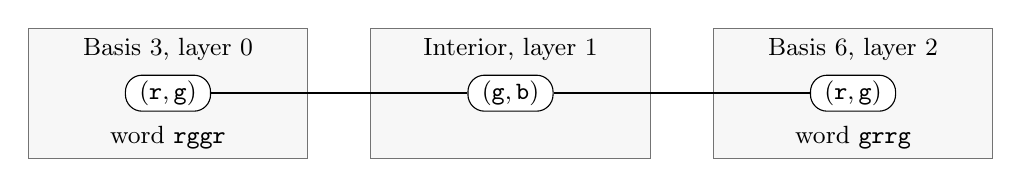
\begin{tikzpicture}[x=1cm,y=1cm,
    layer/.style={draw=black!55,fill=black!3,minimum width=3.55cm,minimum height=1.65cm},
    vertex/.style={draw=black,fill=white,rounded corners=6pt,inner xsep=5pt,inner ysep=2pt},
    every node/.style={font=\small}]
  \foreach \x in {-4.35,0,4.35} \node[layer] at (\x,0) {};
  \node at (-4.35,.56) {Basis 3, layer $0$};
  \node at (0,.56) {Interior, layer $1$};
  \node at (4.35,.56) {Basis 6, layer $2$};
  \node[vertex] (left) at (-4.35,0) {$(\col r,\col g)$};
  \node[vertex] (middle) at (0,0) {$(\col g,\col b)$};
  \node[vertex] (right) at (4.35,0) {$(\col r,\col g)$};
  \draw[semithick] (left.east)--(middle.west) (middle.east)--(right.west);
  \node at (-4.35,-.56) {word $\col{rggr}$};
  \node at (4.35,-.56) {word $\col{grrg}$};
\end{tikzpicture}
\caption{The wire between bases $3$ and $6$ for $H=K_3$ and $\lambda=1$. Each box holds nine vertices, one for every ordered pair of colors. The three marked vertices form a path because both entries change across each drawn edge. At the endpoints, the first entry of $(\col r,\col g)$ occupies positions $\{0,3\}$ in basis $3$ and $\{1,2\}$ in basis $6$. The two endpoint vertices are the vertex $u$ of Section~\ref{sec:example} and the vertex in basis $6$ carrying the same measurement.}
\label{fig:wire}
\end{figure}

We now lift any quantum $3$-coloring of $H$ to $S_\lambda(H)$ at a factor-of-four cost in local dimension. Let $(P_{x,a})_{a\in\mathbb Z/3}$, for $x\in V(H)$, be a quantum $3$-coloring of $H$ on $\C^d$; we call it the input coloring. Its \emph{lift} consists of projectors $P'_{v,a}$ on $\C^4\otimes\C^d$. At a basis word $(i,g)$ and at a wire vertex $(e,\ell,x,y)$, define
\begin{equation}\label{eq:strategy}
 P'_{(i,g),a}=\sum_{s=0}^3 Q^i_s\otimes P_{g_s,a},
 \qquad
 P'_{(e,\ell,x,y),a}
 =P_e\otimes P_{x,a}+(I-P_e)\otimes P_{y,a}.
\end{equation}
Operationally, the first formula measures basis $i$ on $\C^4$ and then applies the measurement of the selected entry $g_s$ on $\C^d$; the second measures the binary plane observable $\{P_e,I-P_e\}$ and applies the measurement of $x$ or $y$ accordingly. By~\eqref{eq:planes} and the definition of $A_{b,e}$, the two formulas agree at every wire endpoint, including both ends of the complemented edge $36$ of $K_{3,3}$. Each formula defines a projective measurement because its first-factor projections are pairwise orthogonal and sum to $I$. On an edge inside a basis chart, the edge rule $P'_{(i,g),a}P'_{(i,g'),a}=0$ holds separately in each of the four orthogonal summands $Q^i_s$; on a wire edge, it holds separately on the range and kernel of $P_e$.

The next lemma shows that~\eqref{eq:strategy} preserves $R$-compatibility whenever $R\le\lambda+2$.

\begin{lemma}\label{lem:radius-lift}
If the coloring of $H$ is $R$-compatible and $R\le\lambda+2$, then~\eqref{eq:strategy} gives an $R$-compatible quantum $3$-coloring of $S_\lambda(H)$.
\end{lemma}
\begin{proof}
Let $u,v\in V(S_\lambda(H))$ satisfy $\dist_{S_\lambda(H)}(u,v)\le R$, and fix a shortest path $\gamma$ of length at most $R$ between $u$ and $v$. For a basis $b$, a \emph{wire at $b$} is a wire along an edge of $K_{3,3}$ that contains $b$. Its vertices include those of both end layers, also the ones that are identified with words of the other basis chart. We claim that there is a basis $b\in\{1,\ldots,6\}$ such that every vertex of $\gamma$ lies in basis chart $b$ or on a wire at $b$. There are three cases, according to the number of basis charts that $\gamma$ visits.
\begin{itemize}
\item If $\gamma$ visits no basis chart, all its vertices lie in the interior of a single wire $e$, because distinct wires meet only at basis charts. Either end of $e$ can serve as $b$.
\item If $\gamma$ visits exactly one basis chart, every wire met by $\gamma$ is a wire at the basis of that chart, and this basis is $b$.
\item Suppose that $\gamma$ visits at least two basis charts. Choose a minimal subpath of $\gamma$ that connects two distinct basis charts, with no chart vertex in between. It traverses a wire $e$ from layer $0$ to layer $\lambda+1$ and has at least $\lambda+1$ edges. Since $\gamma$ has at most $R\le\lambda+2$ edges, at most one edge of $\gamma$ lies outside this subpath.
  \begin{itemize}
  \item If there is no such edge, all vertices of $\gamma$ lie on $e$, and either end of $e$ can serve as $b$.
  \item If there is one, it is attached to one end of the subpath. Let $b$ be the basis at that end. The additional vertex is adjacent to a word of basis chart $b$, so it lies in basis chart $b$ or on a wire at $b$. For $\lambda=0$ and $R=2$ it may be a word of a third basis chart, at the far end of a second wire at $b$.
  \end{itemize}
\end{itemize}

This proves the claim. It implies that the measurement~\eqref{eq:strategy} of every vertex of $\gamma$ is diagonal in basis $b$ in the first tensor factor. Indeed, for any wire $e$ at $b$ we have $P_e=\sum_{s\in A_{b,e}} Q^b_s$ and $I-P_e=\sum_{s\notin A_{b,e}} Q^b_s$ by~\eqref{eq:planes}. Hence every vertex $w$ along $\gamma$ can be written in the form
\[
 P'_{w,a}=\sum_{s=0}^3 Q^b_s\otimes P_{\alpha_s(w),a},
\]
where $\alpha_s(w)\in V(H)$ is $g_s$ if $w=(b,g)$ lies in chart $b$, and equals $x$ for $s\in A_{b,e}$ and $y$ for $s\notin A_{b,e}$ if $w=(e,\ell,x,y)$ lies on a wire $e$ at $b$. Across every edge of $\gamma$, whether inside chart $b$ or along a wire at $b$, the adjacency rules of $S_\lambda(H)$ force $\alpha_s(w)\sim_H \alpha_s(w')$ at each fixed position $s\in\{0,1,2,3\}$. Therefore, for each $s$, the sequence of labels $\alpha_s(w)$ along $\gamma$ is a walk in $H$ of length at most $R$, so $\dist_H(\alpha_s(u),\alpha_s(v))\le R$. Because the input coloring of $H$ is $R$-compatible, $P_{\alpha_s(u),a}$ and $P_{\alpha_s(v),a'}$ commute for all outcomes $a,a'$ and every $s$. Since the four projections $Q^b_s$ are pairwise orthogonal, $P'_{u,a}$ and $P'_{v,a'}$ commute for all $a,a'$.
\end{proof}

For $H=K_3$, the input coloring consists of the \emph{scalar projectors} $P_{x,a}=\mathbf 1_{x=a}$ on $\C^1$ (local dimension $d=1$). Equation~\eqref{eq:strategy} then gives a strategy in local dimension $4$ that reproduces Section~\ref{sec:example}: at $(i,g)$, measure basis $i$ on two qubits and return the color $g_s$ at the obtained position $s$; at a wire vertex $(e,\ell,x,y)$, return $x$ on $P_e$ and $y$ on $I-P_e$.

\subsection{Five classical colors without topology}\label{sec:five}

We now show by a purely combinatorial argument that $\chi(S_\lambda(K_3))=5$ for every $\lambda\ge0$. The proof relies on three rigidity properties of proper $4$-colorings of the categorical powers $K_3^{\times2}$ and $K_3^{\times3}$, where vertices are pairs or triples of colors and two tuples are adjacent precisely when they differ in every coordinate.

Call the nine vertices of $K_3^{\times2}$ \emph{cells}, and arrange them in a $3\times3$ grid: three cells sharing their first coordinate form a \emph{row} of the grid, and three cells sharing their second coordinate form a \emph{column}. In any proper coloring of $K_3^{\times2}$, two cells of the same color must agree in at least one coordinate. Consequently, any color class containing two cells in the same row lies entirely in that row; we call such a color class a \emph{row class}, and define a \emph{column class} symmetrically. A proper coloring of $K_3^{\times2}$ \emph{reads the first coordinate} if some column consists entirely of cells belonging to row classes, and \emph{reads the second coordinate} if some row consists entirely of cells belonging to column classes. For example, the $3$-coloring $(x,y)\mapsto x$ reads the first coordinate.

\begin{lemma}[Four colors read one coordinate]\label{lem:four-colorings}
\leavevmode
\begin{enumerate}
\item[(a)] Every proper $4$-coloring of $K_3^{\times2}$ reads exactly one of the two coordinates.
\item[(b)] Let $f,g$ be proper colorings of $K_3^{\times2}$ with colors from the same set of four colors, such that $f(u)\ne g(v)$ whenever the cells $u,v$ differ in both coordinates. Then $f$ and $g$ read the same coordinate.
\item[(c)] Let $f$ be a proper $4$-coloring of $K_3^{\times3}$. For $m=1,2,3$, let $f_m(x,y)$ be the color of the triple with $x$ in coordinate $m$ and $y$ in the other two coordinates. Then exactly one of the three colorings $f_1,f_2,f_3$ of $K_3^{\times2}$ reads the first coordinate.
\end{enumerate}
\end{lemma}

The analytical proof of Lemma~\ref{lem:four-colorings} is given in Appendix~\ref{app:k3-four}. (Lemma~\ref{lem:four-colorings} is related to the case $t=3$ of~\cite[Lemma~3.7]{BG}, which is not imported here.)

For a basis $i$ and $\{r,s,t\}=\{1,2,3\}$, the partition $\{A_r,\{s\},\{t\}\}$ of the four positions, taken together with the basis $i$, is a \emph{ternary template} at basis $i$. Every basis has three ternary templates, so there are eighteen in all. In the basis chart of $S_\lambda(K_3)$ at $i$, the $27$ words that are constant on $A_r$ induce a copy of $K_3^{\times3}$ indexed by the three parts $A_r,\{s\},\{t\}$, because two such words differ in all four positions precisely when they take different colors on all three parts.

\begin{theorem}[One substitution]\label{thm:one-level}
For every $\lambda\ge0$, the graph $S_\lambda(K_3)$ has quantum chromatic number three, with a $(\lambda+2)$-compatible quantum $3$-coloring in local dimension four, and classical chromatic number five.
\end{theorem}

The idea of the lower bound is this. A proper $4$-coloring of $S_\lambda(K_3)$ would assign a single position $\sigma(i)$ to each basis and thereby assign every observable in~\eqref{eq:pauli-square} a basis-independent sign $\pm1$; the fifth color is what classical players need to evade this commitment. For three colors the obstruction is immediate, because every proper $3$-coloring of $K_3^{\times3}$ depends on a single coordinate (Appendix~\ref{app:k3-powers}).

\begin{proof}
We establish the quantum coloring, exclude classical $4$-colorings via Lemmas~\ref{lem:four-colorings} and~\ref{lem:parity}, and verify that five colors suffice.

\emph{Quantum $3$-coloring.} The scalar projectors on $K_3$ commute at every distance, so Lemma~\ref{lem:radius-lift} applied with $R=\lambda+2$ yields a $(\lambda+2)$-compatible quantum $3$-coloring of $S_\lambda(K_3)$ in local dimension four. The three constant words in any single basis chart form a triangle, so $\cq(S_\lambda(K_3))=3$.

\emph{Four colors do not suffice.} Suppose for contradiction that $f$ is a proper $4$-coloring of $S_\lambda(K_3)$. Let $D$ be any part of a ternary template, that is, one of the six sets $A_1,A_2,A_3,\{1\},\{2\},\{3\}$. For each basis $i\in\{1,\ldots,6\}$ and each pair $(x,y)\in V(K_3)^2$, let $f^i_D(x,y)$ be the color under $f$ of the word in basis chart $i$ that equals $x$ on $D$ and $y$ on $D^c$. Every such word is constant on at least one $A_r$ and therefore belongs to basis chart $i$. Pairs $(x,y)$ and $(x',y')$ differing in both coordinates yield words differing in all four positions, so $f^i_D$ is a proper $4$-coloring of $K_3^{\times2}$. We say that $f$ \emph{reads $D$ at basis $i$} if $f^i_D$ reads the first coordinate.

Fix a basis $i$. On the $27$ words constant on $A_r$ (forming a copy of $K_3^{\times3}$ for the ternary template $\{A_r,\{s\},\{t\}\}$), the three derived colorings of Lemma~\ref{lem:four-colorings}(c) are precisely $f^i_{A_r}$, $f^i_{\{s\}}$, and $f^i_{\{t\}}$. By Lemma~\ref{lem:four-colorings}(c), $f$ reads exactly one part of each of the three ternary templates at basis $i$:
\begin{itemize}
\item If $f$ reads some singleton $\{t\}$ ($t\in\{1,2,3\}$), then the two templates containing $\{t\}$ force $f$ to read none of $A_r,A_s,\{r\},\{s\}$, and the third template $\{A_t,\{r\},\{s\}\}$ forces $f$ to read $A_t$. Set $\sigma(i)=t$.
\item If $f$ reads no singleton, then each template forces $f$ to read its doubleton part, so $f$ reads $A_1$, $A_2$, and $A_3$. Set $\sigma(i)=0$.
\end{itemize}
In both cases, for all six sets $D\in\{A_1,A_2,A_3,\{1\},\{2\},\{3\}\}$,
\begin{equation}\label{eq:selected-position}
 f\text{ reads }D\text{ at basis }i\quad\Longleftrightarrow\quad \sigma(i)\in D.
\end{equation}

Now fix an edge $e=ik$ of $K_{3,3}$ (with $i\le3<k$). For each layer $\ell\in\{0,\ldots,\lambda+1\}$ of the wire along $e$, let $h_\ell(x,y)$ denote the color under $f$ of the vertex $(x,y)$ in layer $\ell$. Each $h_\ell$ is a proper $4$-coloring of $K_3^{\times2}$, and consecutive layers $h_\ell,h_{\ell+1}$ satisfy the cross-edge hypothesis of Lemma~\ref{lem:four-colorings}(b). By induction along the wire, $h_0$ and $h_{\lambda+1}$ read the same coordinate. At layer $0$, the endpoint identification gives $h_0=f^i_{A_{i,e}}$, so by~\eqref{eq:selected-position}
\[
 h_0\text{ reads the first coordinate}\quad\Longleftrightarrow\quad\sigma(i)\in A_{i,e}.
\]
Suppose first that $e\ne36$. Then $A_{k,e}=A_r$ for some $r$ and $h_{\lambda+1}=f^k_{A_{k,e}}$, so by~\eqref{eq:selected-position}
\[
 h_{\lambda+1}\text{ reads the first coordinate}\quad\Longleftrightarrow\quad\sigma(k)\in A_{k,e}.
\]
Now let $e=36$, so that $A_{6,36}=A_3^c$. The endpoint identification places $x$ on $A_3^c$ and $y$ on $A_3$, so $h_{\lambda+1}(x,y)=f^6_{A_3}(y,x)$. Thus $h_{\lambda+1}$ reads the first coordinate precisely when $f^6_{A_3}$ reads the second. By Lemma~\ref{lem:four-colorings}(a), this happens precisely when $f^6_{A_3}$ does not read the first coordinate, that is, by~\eqref{eq:selected-position}, when $\sigma(6)\notin A_3$. Hence
\[
 h_{\lambda+1}\text{ reads the first coordinate}\quad\Longleftrightarrow\quad\sigma(6)\in A_3^c=A_{6,36}.
\]
In both cases, since $h_0$ and $h_{\lambda+1}$ read the same coordinate, we obtain $\sigma(i)\in A_{i,e}$ if and only if $\sigma(k)\in A_{k,e}$, for every edge $e=ik$ of $K_{3,3}$. This contradicts Lemma~\ref{lem:parity}. Hence $\chi(S_\lambda(K_3))\ge5$.

\emph{Five colors suffice.} Mapping each vertex of $S_\lambda(K_3)$ to its projective measurement~\eqref{eq:strategy} gives a graph homomorphism into the physical graph of all three-label measurements formed from the six bases. Proposition~\ref{prop:physical-upper} in Appendix~\ref{app:five-coloring} (applied with $n=3$) properly colors that physical graph with five colors. Therefore $\chi(S_\lambda(K_3))=5$.
\end{proof}

\subsection{Generalizing to arbitrary triads}\label{sec:one-in-three}

The proof of Theorem~\ref{thm:one-level} uses nothing specific to two qubits beyond Lemma~\ref{lem:four-colorings} and the absence of a consistent choice of one ray per basis. We now isolate this mechanism for arbitrary sets of three-outcome projective measurements; Section~\ref{sec:alldim} applies it to Peres' $33$ rays in $\R^3$ to obtain graphs with $(\cq,\chi)=(3,5)$ admitting quantum $3$-colorings in local dimension three at every compatibility radius.

Let $\mathcal D$ be a finite nonempty set of \emph{triads}, where a triad is an unordered triple $\{E_1,E_2,E_3\}$ of nonzero orthogonal projections on $\C^d$ summing to $I$. We call $E_1,E_2,E_3$ the \emph{parts} of the triad. Because its three parts are nonzero and sum to $I$, a triad contains at most one member of any complementary pair $\{P,I-P\}$. A \emph{one-in-three selection} for $\mathcal D$ chooses exactly one part in every triad such that, across distinct triads, two equal parts are either both chosen or both unchosen, and of two complementary parts exactly one is chosen.

For an integer $\lambda\ge0$, the graph $W_\lambda(\mathcal D)$ is built from charts and wires in the same way as $S_\lambda(K_3)$.
\begin{itemize}
\item \emph{Charts.} Each triad $T\in\mathcal D$ has a \emph{chart} of $27$ words, which assign one of the three colors to each of its three parts. Two words of the same chart are adjacent whenever they differ on all three parts.
\item \emph{Wires.} For every complementary pair $\{P,I-P\}$ that occurs among the parts of $\mathcal D$, fix an ordering of the triads that contain $P$ or $I-P$. Let $T_1$ be the first of these triads, with part $P_1\in\{P,I-P\}$. The chart of $T_1$ is connected to the chart of every other triad $T$ in the list by a \emph{wire} of layers $\ell=0,\ldots,\lambda+1$, each a copy of $V(K_3)^2$. Within a wire, $(x,y)$ and $(x',y')$ in equal or consecutive layers are adjacent whenever $x\ne x'$ and $y\ne y'$.
\item \emph{Identifications.} The pair $(x,y)$ in layer $0$ is identified with the word of $T_1$ that assigns $x$ to $P_1$ and $y$ to the other two parts. The pair $(x,y)$ in layer $\lambda+1$ is identified with the word of $T$ that carries the same measurement: if $T$ contains $P_1$, this word assigns $x$ to $P_1$ and $y$ to the other two parts of $T$; if $T$ contains $I-P_1$, it assigns $y$ to $I-P_1$ and $x$ to the other two parts of $T$.
\item \emph{Measurements.} A chart word carries the projective measurement whose projector for a color $a$ is the sum of the parts colored $a$. A wire vertex $(x,y)$ carries the measurement that returns $x$ on $P_1$ and $y$ on $I-P_1$.
\end{itemize}
The graph $W_\lambda(\mathcal D)$ depends on the chosen orderings of the triads, but the following result holds for every choice.

\begin{proposition}[One-in-three configurations]\label{prop:one-in-three}
These measurements form a $(\lambda+2)$-compatible quantum $3$-coloring of $W_\lambda(\mathcal D)$ in local dimension $d$, and $\cq(W_\lambda(\mathcal D))=3$. If $\mathcal D$ has no one-in-three selection, then $\chi(W_\lambda(\mathcal D))\ge5$.
\end{proposition}
\begin{proof}
\emph{Edge rule and $\cq=3$.} On a chart edge, the two projectors for any fixed color $a$ sum over disjoint subsets of the triad's parts and are orthogonal. On a wire edge, the two projectors for color $a$ are orthogonal separately on the range of $P_1$ and on the range of $I-P_1$. Thus the displayed measurements form a quantum $3$-coloring in local dimension $d$. The three constant words of any chart form a triangle, so $\cq(W_\lambda(\mathcal D))=3$.

\emph{$(\lambda+2)$-compatibility.} Call a projective measurement a \emph{coarse-graining} of a triad $T$ if each of its projectors is a sum of parts of $T$; any two coarse-grainings of the same triad commute. Every word in the chart of $T$ is a coarse-graining of $T$, and every vertex on a wire connecting two triads is a coarse-graining of both endpoint triads. Now consider any path $\gamma$ in $W_\lambda(\mathcal D)$ of length at most $\lambda+2$. Traversing a wire between two distinct charts takes at least $\lambda+1$ edges. Just as in Lemma~\ref{lem:radius-lift}:
\begin{itemize}
\item if $\gamma$ meets at most one chart, all vertices of $\gamma$ lie in a single wire or in one chart together with wires incident to it;
\item if $\gamma$ meets two distinct charts, some subpath traverses a wire completely and leaves at most one additional edge, so every vertex of $\gamma$ lies in the chart at the end carrying that extra edge (or either end if there is none) or on wires incident to it---including the case $\lambda=0$ where two wires meet at a middle chart vertex.
\end{itemize}
In every case, both endpoints of $\gamma$ carry coarse-grainings of a common triad and therefore commute.

\emph{Classical lower bound.} Suppose $f$ is a proper $4$-coloring of $W_\lambda(\mathcal D)$. For a triad $T\in\mathcal D$ and a part $E\in T$, let $f_{T,E}(x,y)$ be the color under $f$ of the word of $T$ taking $x$ on $E$ and $y$ on the other two parts, and say that $f$ \emph{reads $E$ in $T$} if $f_{T,E}$ reads the first coordinate. Because each chart is a copy of $K_3^{\times3}$, Lemma~\ref{lem:four-colorings}(c) implies that $f$ reads exactly one part in every triad.

Fix a complementary pair $\{P,I-P\}$, its first triad $T_1$ with part $P_1$, and any wire from $T_1$ to another triad $T$ with part $E\in\{P_1,I-P_1\}$. By Lemma~\ref{lem:four-colorings}(b), all layers of this wire read the same coordinate. Layer $0$ restricts $f$ to $f_{T_1,P_1}$. Layer $\lambda+1$ restricts $f$ to $f_{T,E}$ if $E=P_1$, and to $(x,y)\mapsto f_{T,E}(y,x)$ if $E=I-P_1$. By Lemma~\ref{lem:four-colorings}(a), $f$ reads $E$ in $T$ if and only if $f$ reads $P_1$ in $T_1$ when $E=P_1$, and if and only if $f$ does not read $P_1$ in $T_1$ when $E=I-P_1$. Because every triad containing $P$ or $I-P$ is joined by a wire to $T_1$, equal parts in distinct triads are either both read or both unread, while complementary parts have exactly one read. Selecting in every triad the unique part read by $f$ therefore gives a one-in-three selection for $\mathcal D$. By contraposition, if $\mathcal D$ admits no one-in-three selection, then $\chi(W_\lambda(\mathcal D))\ge5$.
\end{proof}

The Mermin--Peres square is an example. Its eighteen triads are $\{P^i_r,Q^i_s,Q^i_t\}$, one for each ternary template. They have no one-in-three selection: the case analysis that gave~\eqref{eq:selected-position}, applied to the chosen parts in place of the parts read by a coloring, would turn a selection into a choice of positions that Lemma~\ref{lem:parity} excludes. The graph $S_\lambda(K_3)$ is a more compact realization of $W_\lambda(\mathcal D)$ for these triads, in which the three charts of a basis share their common words. In Section~\ref{sec:alldim}, applying Proposition~\ref{prop:one-in-three} to Peres' lines in $\R^3$ gives explicit qutrit graphs with $(\cq,\chi)=(3,5)$ at every compatibility radius.

\section{Iterating the substitution and the sparse family}\label{sec:iteration}

Applying the square substitution $S_\lambda$ repeatedly starting from $K_3$ lifts the quantum $3$-coloring at a factor-of-four cost in local dimension per level while preserving $(\lambda+2)$-compatibility. Because the full iterate grows doubly exponentially in the number of levels, we also define a sparse induced subgraph $G_{j,R}$. We then introduce the box complex and chain towers to prove that every substitution raises the classical chromatic lower bound by two on both families, and count presentations to bound the size of $G_{j,R}$.

\subsection{Full iterates and bounded presentations}\label{sec:sparse}

For an integer $j\ge0$ and a parameter $\lambda\ge0$, let $S^j_\lambda(H)$ denote the result of applying $S_\lambda$ successively $j$ times to $H$, with $S^0_\lambda(H)=H$. We call $S^j_\lambda(K_3)$ the \emph{full iterate} at \emph{level} $j$ (or the \emph{$j$th iterate}). A vertex at level $j\ge1$ is either a word of four vertices of level $j-1$ in one of the six basis charts, or a pair of level-$(j-1)$ vertices on an interior layer of a wire, as in the level-two vertex $w$ of Section~\ref{sec:example}.

Iterating~\eqref{eq:strategy} $j$ times starting from the scalar projectors on $K_3$ produces projective measurements on $(\C^4)^{\otimes j}$ (local dimension $4^j$). To evaluate a vertex of $S^j_\lambda(K_3)$, a player measures the first two-qubit register in the vertex's basis (or measures $\{P_e,I-P_e\}$ at a wire vertex); the resulting position selects a level-$(j-1)$ vertex, and the player proceeds adaptively on the remaining registers. After $j$ rounds a single color of $K_3$ remains. By~\eqref{eq:pauli-square}, every round measures commuting two-qubit Pauli observables, so the entire strategy uses adaptive Pauli measurements on $2j$ shared EPR pairs.

To extract an induced subgraph whose size grows only singly exponentially in $j$, we represent vertices of the full iterates $S^h_\lambda(K_3)$ by rooted ordered trees. Given a prescribed compatibility parameter $R\ge1$, set $\lambda=\max\{R-2,0\}$. Then $\lambda+2=\max\{R,2\}\ge R$, so every $(\lambda+2)$-compatible coloring is $R$-compatible. In the tree constructions that follow, the three colors $0,1,2$ of $K_3$ are called \emph{scalars}. A \emph{presentation} of a vertex of $S^h_\lambda(K_3)$ at level $h$ is a rooted ordered tree defined inductively as follows:
\begin{itemize}
\item A \emph{leaf} carries a scalar $a\in\{0,1,2\}$. At level $0$ it evaluates to the color $a$ (corresponding to the scalar projectors of Section~\ref{sec:substitution}). At level $h\ge1$ it evaluates to the constant word in basis $6$ on its value at level $h-1$; we say that the scalar is \emph{padded}.
\item An internal node at level $h\ge1$ evaluates its children at level $h-1$ and takes one of two forms:
  \begin{itemize}
  \item A \emph{basis node} specifies a template. This is either a ternary template $\{A_r,\{s\},\{t\}\}$ at a basis $i\in\{1,\ldots,6\}$ (Section~\ref{sec:five}), or the \emph{binary template}, which is the partition $\{A_3,A_3^c\}$ at basis $6$. There are nineteen templates in all: eighteen ternary and one binary. A basis node has one child per part (three for a ternary template, two for the binary template) and evaluates to the word that repeats each child across every position of its part.
  \item A \emph{wire node} specifies an edge $e$ of $K_{3,3}$ and a layer $\ell\in\{0,\ldots,\lambda+1\}$. Its first child may be any presentation at level $h-1$, while its second child---called its \emph{background}---must be a scalar leaf. If its two children evaluate to $x$ and $y$, the wire node evaluates to $(x,y)$ in layer $\ell$ of wire $e$, subject to the endpoint identifications of Section~\ref{sec:substitution}.
  \end{itemize}
\end{itemize}
The children of an internal node are indexed by its parts or by the two wire coordinates, so a child repeated across two positions of a word counts only once as a node of the tree. Figure~\ref{fig:presentation} shows two presentations.

\begin{figure}[htbp]
\centering
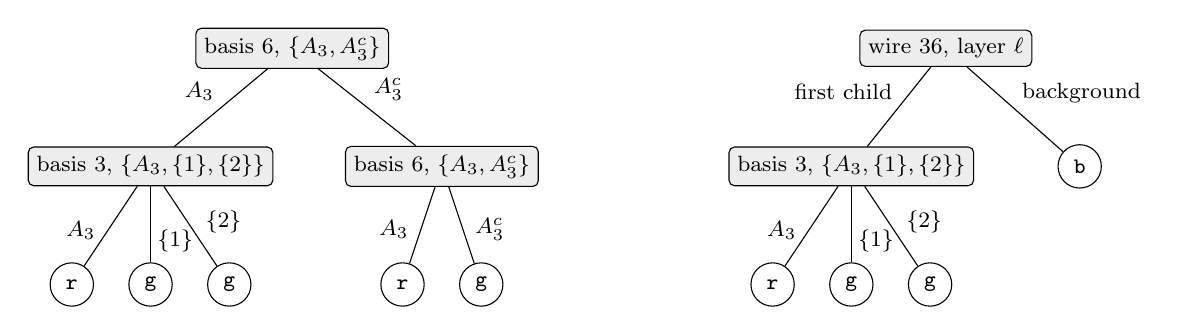
\begin{tikzpicture}[x=1cm,y=1cm,
   inner/.style={draw=black,fill=black!7,rounded corners=2pt,inner xsep=3pt,inner ysep=3pt,font=\footnotesize},
   leaf/.style={draw=black,circle,inner sep=1pt,minimum size=5.5mm,font=\footnotesize},
   every node/.style={font=\footnotesize}]
\begin{scope}
 \node[inner] (w) at (0,0) {basis $6$, $\{A_3,A_3^c\}$};
 \node[inner] (u) at (-1.8,-1.5) {basis $3$, $\{A_3,\{1\},\{2\}\}$};
 \node[inner] (v) at (1.9,-1.5) {basis $6$, $\{A_3,A_3^c\}$};
 \node[leaf] (u1) at (-2.8,-3.0) {$\col r$};
 \node[leaf] (u2) at (-1.8,-3.0) {$\col g$};
 \node[leaf] (u3) at (-0.8,-3.0) {$\col g$};
 \node[leaf] (v1) at (1.4,-3.0) {$\col r$};
 \node[leaf] (v2) at (2.4,-3.0) {$\col g$};
 \draw (w)-- node[above left=-1pt] {$A_3$} (u);
 \draw (w)-- node[above right=-1pt] {$A_3^c$} (v);
 \draw (u)-- node[left=1pt,pos=.55] {$A_3$} (u1);
 \draw (u)-- node[right=-1pt,pos=.72] {$\{1\}$} (u2);
 \draw (u)-- node[right=3pt,pos=.45] {$\{2\}$} (u3);
 \draw (v)-- node[left=1pt,pos=.55] {$A_3$} (v1);
 \draw (v)-- node[right=1pt,pos=.55] {$A_3^c$} (v2);
\end{scope}
\begin{scope}[xshift=8.3cm]
 \node[inner] (n) at (0,0) {wire $36$, layer $\ell$};
 \node[inner] (u) at (-1.2,-1.5) {basis $3$, $\{A_3,\{1\},\{2\}\}$};
 \node[leaf] (b) at (1.7,-1.5) {$\col b$};
 \node[leaf] (u1) at (-2.2,-3.0) {$\col r$};
 \node[leaf] (u2) at (-1.2,-3.0) {$\col g$};
 \node[leaf] (u3) at (-0.2,-3.0) {$\col g$};
 \draw (n)-- node[above left=-1pt] {first child} (u);
 \draw (n)-- node[above right=-1pt] {background} (b);
 \draw (u)-- node[left=1pt,pos=.55] {$A_3$} (u1);
 \draw (u)-- node[right=-1pt,pos=.72] {$\{1\}$} (u2);
 \draw (u)-- node[right=3pt,pos=.45] {$\{2\}$} (u3);
\end{scope}
\end{tikzpicture}
\caption{Two presentations at level $2$, with the colors $\col r,\col g,\col b$ of Section~\ref{sec:example} as scalars. Every edge is labeled by the part, or by the wire coordinate, to which the child belongs. Left: a presentation of the vertex $w=\bigl(6,(u,v,v,u)\bigr)$ of Section~\ref{sec:example}. The root is a basis node with the binary template at basis $6$, and its two children present $u=(3,\col{rggr})$ and $v=(6,\col{rggr})$. The tree has three internal nodes and no wire node. Right: a presentation of a vertex in layer $\ell$ of the wire along the edge $36$. The first child of the wire node presents $u$. The background of the wire node is the scalar $\col b$, which sits at level $1$ and is therefore padded to the constant word $\col{bbbb}$ in basis $6$. The tree has two internal nodes, one of which is a wire node.}
\label{fig:presentation}
\end{figure}

\begin{definition}\label{def:sparse-graph}
For $j,R\ge1$ and $\lambda=\max\{R-2,0\}$, let $G_{j,R}$ be the subgraph of $S^j_\lambda(K_3)$ induced by the vertices admitting a presentation with at most $2j-1$ internal nodes and at most $j$ wire nodes.
\end{definition}

We call $(G_{j,R})$ the \emph{sparse family}. Distinct presentations evaluating to the same vertex of $S^j_\lambda(K_3)$ produce a single vertex of $G_{j,R}$, and $G_{j,R}$ retains every edge of the full iterate between its vertices, including edges between vertices described by different trees. At level $j=1$, every vertex of $S_\lambda(K_3)$ has a presentation with a single internal node---a ternary basis node for a word of a basis chart, a wire node for a vertex of an interior layer---so $G_{1,R}=S_\lambda(K_3)$.

\subsection{The box complex and its first Stiefel--Whitney class}\label{sec:box}

To bound $\chi(S^j_\lambda(K_3))$ and $\chi(G_{j,R})$ from below at every level $j$, we use an equivariant topological invariant of graphs~\cite{Mat,Kozlov}. Every proper coloring sends the two sides of any complete bipartite subgraph to disjoint color sets; the box complex organizes all such bipartite pairs into a single topological space.

For a finite loopless graph $H$, the \emph{box complex} $\B(H)$ is the space of all ordered pairs $(\mu,\nu)$ of probability measures on $V(H)$ such that every vertex in $\operatorname{supp}\mu$ is adjacent in $H$ to every vertex in $\operatorname{supp}\nu$. It carries the subspace topology inherited from the product of two probability simplices. The two supports $\operatorname{supp}\mu$ and $\operatorname{supp}\nu$ are called the \emph{shores} of $(\mu,\nu)$.

Because $H$ is loopless, the two shores are disjoint, so swapping them, $(\mu,\nu)\mapsto(\nu,\mu)$, is a free continuous involution on $\B(H)$. A continuous map between spaces with involutions is \emph{equivariant} if it commutes with the involutions. Any graph homomorphism $f:G\to H$ induces an equivariant continuous map $\B(G)\to\B(H)$ by pushing both probability measures forward along $f$.

The space $\B(H)$ is the complex $\operatorname{Hom}(K_2,H)$ (surveyed in~\cite{Kozlov}), which is one of several models of the box complex. For connected graphs, Csorba~\cite[Theorem~9]{Csorba} shows that the barycentric subdivision of the simplicial box complex of Matou{\v s}ek and Ziegler~\cite{MZ} collapses equivariantly onto that of $\operatorname{Hom}(K_2,H)$. The two models are therefore equivariantly homotopy equivalent, so both admit the same equivariant maps to spheres and carry the same Stiefel--Whitney class defined below.

For the complete graph $K_p$ ($p\ge2$), two shores are completely adjacent precisely when they are disjoint. Consequently, the map $(\mu,\nu)\mapsto\mu-\nu$ identifies $\B(K_p)$ homeomorphically with the $\ell_1$-sphere of radius $2$ in the $(p-1)$-dimensional hyperplane $\{x\in\R^p:\sum_{a=1}^p x_a=0\}$, with inverse taking normalized positive and negative parts. Radial projection identifies this sphere equivariantly with the Euclidean $(p-2)$-sphere $S^{p-2}$ carrying the antipodal involution. Every proper $p$-coloring $H\to K_p$ therefore induces an equivariant continuous map $\B(H)\to S^{p-2}$. For $p=3$, the space $\B(K_3)$ is a hexagon---homeomorphic to the circle $S^1$ with shore exchange acting as the antipodal half-turn.

Any free involution $T$ on a compact polyhedron $Z$ defines a double cover $Z\to Z/\{1,T\}$ and hence a cohomology class $w_Z\in H^1(Z/\{1,T\};\Ftwo)$, the \emph{first Stiefel--Whitney class} of the double cover~\cite{MS}. Evaluated on a closed loop in $Z/\{1,T\}$, the class $w_Z$ equals $1$ if a lift of the loop to $Z$ switches sheets and $0$ if it closes up. An equivariant map $Z\to Y$ pulls back $w_Y$ to $w_Z$. In particular, if $Z$ admits an equivariant map to $\B(H)$ and $w_Z^k\ne0$ in $H^k(Z/\{1,T\};\Ftwo)$, then
\begin{equation}\label{eq:classical-obstruction}
 \chi(H)\ge k+2.
\end{equation}
Indeed, composing $Z\to\B(H)$ with the equivariant map $\B(H)\to S^{p-2}$ from a $p$-coloring descends to a map $Z/\{1,T\}\to\mathbb{RP}^{p-2}$ pulling back the generator of $H^1(\mathbb{RP}^{p-2};\Ftwo)$ to $w_Z$. Since $H^k(\mathbb{RP}^{p-2};\Ftwo)=0$ for $k>p-2$, $w_Z^k\ne0$ forces $p-2\ge k$, i.e., $p\ge k+2$. For $Z=\B(H)$, we write simply $w=w_{\B(H)}$ and call the largest integer $k$ with $w^k\ne0$ the \emph{height} of $w$.

\subsection{Towers and the substitution step}\label{sec:towers}

To lift the obstruction~\eqref{eq:classical-obstruction} inductively across each substitution, we mirror the graph operation $S_\lambda$ on topological spaces carrying a free circle action.

A \emph{circle space} is a compact polyhedron $X$ equipped with a free continuous action of the circle group $S^1=\{z\in\C:|z|=1\}$. Its \emph{half-turn} is the action $T(x)=(-1)\cdot x$, which is a free involution on $X$. Given a circle space $X$, the space $S(X)$ is defined in the same way as the graph $S_\lambda(H)$.
\begin{itemize}
\item \emph{Basis blocks.} A \emph{basis block} is the subspace of tuples $(x_0,x_1,x_2,x_3)\in X^4$ that satisfy $x_0=x_r$ for some $r\in\{1,2,3\}$. Take six disjoint basis blocks, one for each basis $i\in\{1,\ldots,6\}$.
\item \emph{Cylinders.} For each edge $e=ik$ of $K_{3,3}$ (with $i\le3<k$), take a cylinder $X^2\times[0,1]$.
\item \emph{Attachments.} For each edge $e=ik$, identify the point $(x,y,0)$ of its cylinder with the tuple in basis block $i$ that takes $x$ on $A_{i,e}$ and $y$ on $A_{i,e}^c$, and identify the point $(x,y,1)$ with the tuple in basis block $k$ that takes $x$ on $A_{k,e}$ and $y$ on $A_{k,e}^c$. These are the coordinate repetitions of $S_\lambda$.
\end{itemize}
Rotating all coordinates simultaneously defines a free continuous $S^1$-action, which makes $S(X)$ a circle space (verified in Appendix~\ref{app:cont-pres}).

Work with normalized singular chains over $\Ftwo$. For a chain $c$ in a circle space, let $Bc$ denote the chain swept out by $c$ during one full rotation of $S^1$ (defined precisely via the shuffle chain action before~\eqref{eq:circle-chain} in Appendix~\ref{app:cont-pres}). A \emph{tower of length $h$} on a circle space $Z$ consists of a $0$-chain $x_0$ given by a single point together with chains $x_1,\ldots,x_h$, where $x_i$ has dimension $2i$, satisfying
\begin{equation}\label{eq:tower}
 \partial x_i=Bx_{i-1}\qquad (1\le i\le h).
\end{equation}
Thus a tower of length $0$ is simply a point, and a tower of length $1$ is a point together with a $2$-chain whose boundary is the $S^1$-orbit of that point. A \emph{tower of length $h$ over a graph $G$} consists of a circle space $Z$ with a tower of length $h$ together with a continuous map $Z\to\B(G)$ that is equivariant for the half-turn $T$ on $Z$ and shore exchange on $\B(G)$. We say that a circle space (or graph) \emph{carries} a tower of length $h$ if such a tower exists on it (respectively, over it).

A tower of length $h$ forces $2h+1$ nonvanishing powers of the Stiefel--Whitney class.

\begin{proposition}[Towers bound the chromatic number]\label{prop:tower-bound}
If there is a tower of length $h$ over $G$, then $w^{2h+1}\ne0$ on $\B(G)$ and $\chi(G)\ge2h+3$.
\end{proposition}
\begin{proof}
Let $Z\to\B(G)$ be the equivariant map of a tower of length $h$ over $G$. Lemma~\ref{lem:tower-detection} in Appendix~\ref{app:tower-det} shows that $w_Z^{2h+1}\ne0$. Because $w_Z$ is the pullback of $w$ along $Z\to\B(G)$, we also have $w^{2h+1}\ne0$ on $\B(G)$. Applying~\eqref{eq:classical-obstruction} with $k=2h+1$ yields $\chi(G)\ge2h+3$.
\end{proof}

The heart of our classical lower bound is that each square substitution extends any tower by one step.

\begin{theorem}[Substitution step]\label{thm:step}
If there is a tower of length $h$ over a graph $H$, on a circle space $X$, then for every $\lambda\ge0$ there is a tower of length $h+1$ over $S_\lambda(H)$, on the circle space $S(X)$. Consequently, for every $j\ge0$,
\[
 w^{2(h+j)+1}\ne0\ \text{ on }\B(S^j_\lambda(H)),\qquad \chi(S^j_\lambda(H))\ge2(h+j)+3.
\]
\end{theorem}
\begin{proof}
Let $x_0,\ldots,x_h$ be a tower of length $h$ on $X$ with equivariant map $X\to\B(H)$. Appendix~\ref{app:cont-pres} shows that $S(X)$ is a circle space. Lemma~\ref{lem:square-tower}(a) in Appendix~\ref{app:cont-pres} produces a tower of length $h+1$ on $S(X)$, and Lemma~\ref{lem:box-realization} in Appendix~\ref{app:box-real} lifts $X\to\B(H)$ to an equivariant map $S(X)\to\B(S_\lambda(H))$. Together these form a tower of length $h+1$ over $S_\lambda(H)$. Applying this step $j$ times produces a tower of length $h+j$ over $S^j_\lambda(H)$, and Proposition~\ref{prop:tower-bound} yields both displayed conclusions.
\end{proof}

Before turning to the applications, we explain the cancellation behind Lemma~\ref{lem:square-tower}. Consider first a tower of length $0$, which is a single point $x_0$ of $X$. A tower of length $1$ on $S(X)$ consists of a point of $S(X)$ and a $2$-chain whose boundary is the $S^1$-orbit of that point. The point will be the constant tuple $(x_0,x_0,x_0,x_0)$ in basis block $6$, and we have to show that its orbit is a boundary over $\Ftwo$.

Let $b$ be a basis, and let $D$ be either a part of a template at $b$ or the set $\{0,1,2,3\}$ of all positions. Let $\gamma_{b,D}$ be the loop in basis block $b$ along which the entries at the positions in $D$ run once around the orbit of $x_0$, while the other entries stay at $x_0$. For $D=\{0,1,2,3\}$ this loop is the orbit of the constant tuple of block $b$, and we denote it by $o_b$. In homology with coefficients in $\Ftwo$, the loops satisfy two kinds of relations.
\begin{itemize}
\item \emph{Templates.} A template at $b$ with parts $D_1,\ldots,D_p$ defines a map from $X^p$ into block $b$, which repeats its $m$th argument at the positions of $D_m$. This map sends the product of $p$ copies of the orbit of $x_0$ onto a torus. On a torus, the diagonal loop is homologous to the sum of the coordinate loops. Hence $o_b$ is homologous to $\gamma_{b,D_1}+\cdots+\gamma_{b,D_p}$.
\item \emph{Wires.} The cylinder of an edge $e=ik$ carries the loop $\gamma_{i,A_{i,e}}$ to the loop $\gamma_{k,A_{k,e}}$, and the orbit $o_i$ to the orbit $o_k$. Hence $\gamma_{i,A_{i,e}}$ is homologous to $\gamma_{k,A_{k,e}}$, and all six orbits $o_b$ are homologous to one another.
\end{itemize}
Now add the relations of all nineteen templates. On the left there are nineteen orbits. On the right, the loops occur as follows.
\[
\begin{array}{c|c|c}
\text{Basis }b & \text{Loops that occur twice} & \text{Loops that occur once}\\ \hline
1,\ldots,5 & \gamma_{b,\{1\}},\ \gamma_{b,\{2\}},\ \gamma_{b,\{3\}} & \gamma_{b,A_1},\ \gamma_{b,A_2},\ \gamma_{b,A_3}\\
6 & \gamma_{6,\{1\}},\ \gamma_{6,\{2\}},\ \gamma_{6,\{3\}},\ \gamma_{6,A_3} & \gamma_{6,A_1},\ \gamma_{6,A_2},\ \gamma_{6,A_3^c}
\end{array}
\]
At every basis, each singleton belongs to two of the three ternary templates and each set $A_r$ to one of them. At basis $6$, the binary template $\{A_3,A_3^c\}$ contributes $\gamma_{6,A_3}$ a second time and adds $\gamma_{6,A_3^c}$. Loops that occur twice cancel modulo $2$. By Table~\ref{tab:edges}, the eighteen loops that occur once are exactly the loops $\gamma_{b,A_{b,e}}$ at the two ends of the nine edges $e$ of $K_{3,3}$, so they cancel in pairs along the wires. The right-hand side therefore vanishes in homology. Since nineteen is odd and the orbits $o_b$ are homologous to one another, the left-hand side is homologous to $o_6$. Thus $o_6$ is a boundary, as required. Without the binary template the count would prove nothing: the loops $\gamma_{3,A_3}$ and $\gamma_{6,A_3}$ would remain unpaired, and the number of orbits would be even.

For a tower $x_0,\ldots,x_h$ of arbitrary length, Lemma~\ref{lem:square-tower} carries out the same count with chains in place of loops. For each of the nineteen templates it forms a product of the chains of the tower over the parts of the template. The boundary terms that do not cancel within one template are \emph{insertions}: the chain $Bx_h$, swept out by the last chain of the tower, placed on a single part $D$ at a basis $b$, with the base point $x_0$ at all other positions. Insertions cancel as the loops $\gamma_{b,D}$ do in the array above. Those that occur twice cancel modulo $2$, and the remaining eighteen are the two ends of the nine cylinders $X^2\times[0,1]$, along which the inserted chain is swept. In dimension $0$, the constant tuple on $x_0$ occurs $3+3$ times in each of the blocks $1,\ldots,5$, from three templates and three wire ends, and $4+3$ times in block $6$. Over $\Ftwo$ only the constant tuple in block $6$ remains, and it is the base point of the new tower.

\subsection{The chromatic gap and sparse size bounds}\label{sec:gap-results}

All pieces are now in place to prove the chromatic gap for the full iterates $S^j_\lambda(K_3)$ and for the sparse family $G_{j,R}$.

\begin{theorem}[The gap]\label{thm:gap}
For all $j\ge1$ and $\lambda\ge0$, the graph $S^j_\lambda(K_3)$ has quantum chromatic number three and classical chromatic number at least $2j+3$. The strategy above is a $(\lambda+2)$-compatible quantum $3$-coloring in local dimension $4^j$.
\end{theorem}
\begin{proof}
\emph{Quantum $3$-coloring.} The scalar projectors on $K_3$ commute at every distance. Applying Lemma~\ref{lem:radius-lift} inductively $j$ times with $R=\lambda+2$ shows that the $j$-fold iterate of~\eqref{eq:strategy} is a $(\lambda+2)$-compatible quantum $3$-coloring of $S^j_\lambda(K_3)$ in local dimension $4^j$. Moreover, starting from $K_3$, the constant words in any basis chart on the vertices of a triangle again form a triangle; by induction, $S^j_\lambda(K_3)$ contains a triangle, so $\cq(S^j_\lambda(K_3))=3$.

\emph{Classical lower bound.} As shown in Section~\ref{sec:box}, $\B(K_3)$ is a circle on which shore exchange acts as the half-turn. Taking $X=\B(K_3)$ with the identity map and any single point $x_0\in\B(K_3)$ gives a tower of length $h=0$ over $K_3$. Theorem~\ref{thm:step} applied with $h=0$ yields $\chi(S^j_\lambda(K_3))\ge2j+3$.
\end{proof}

Section~\ref{sec:rigidity} proves that neither the local dimension $4^j$ nor the compatibility radius $\lambda+2$ can be improved on $S^j_\lambda(K_3)$.

\begin{remark}\label{rem:tables}
For $\lambda=0$, every vertex of $S^j_0(K_3)$ is a basis word at every level. Its measurement in the $j$-fold iterate of~\eqref{eq:strategy} is therefore that of a \emph{table}. A table chooses one of the six bases for every sequence of fewer than $j$ positions, the empty sequence included; this is the basis in which the next two-qubit register is measured. It also chooses one of the three colors for every sequence of $j$ positions. Let $M_j$ be the physical graph on the measurements of all $6^{(4^j-1)/3}3^{4^j}$ tables. Adjacent vertices of $S^j_0(K_3)$ carry measurements that are orthogonal at every color, hence distinct and adjacent in $M_j$, so $\chi(M_j)\ge\chi(S^j_0(K_3))\ge2j+3$ by Theorem~\ref{thm:gap}. Moreover, $\cq(M_j)=3$, because the measurements themselves form a quantum $3$-coloring of $M_j$ in local dimension $4^j$ and the three constant measurements form a triangle.
\end{remark}

The order of $S^j_\lambda(K_3)$ grows doubly exponentially in $j$, because one substitution turns an $n$-vertex graph into a graph on $6(n^4-n(n-1)^3)+9\lambda n^2$ vertices. Restricting to bounded presentations reduces the order and edge count to singly exponential in $j$ while preserving every property of Theorem~\ref{thm:gap}.

\begin{theorem}[The sparse family]\label{thm:sparse}
There is an absolute constant $C$ such that, for all $j,R\ge1$, the graph $G_{j,R}$ satisfies
\[
 \cq(G_{j,R})=3,\qquad \chi(G_{j,R})\ge2j+3,\qquad |V(G_{j,R})|+|E(G_{j,R})|\le[C(1+R)]^j.
\]
The strategy of Theorem~\ref{thm:gap} restricts to an $R$-compatible quantum $3$-coloring of $G_{j,R}$ in local dimension $4^j$, and $w^{2j+1}\ne0$ on $\B(G_{j,R})$. The graph and the projectors in~\eqref{eq:strategy} can be generated deterministically in $\exp(O(j\log(R+2)))$ bit operations, with an absolute implicit constant.
\end{theorem}
\begin{proof}
We establish in turn the quantum coloring, the topological classical lower bound, the vertex and edge counts, and the deterministic generation bound. Throughout, set $\lambda=\max\{R-2,0\}$.

\emph{Quantum $3$-coloring.} Because $G_{j,R}$ is a subgraph of $S^j_\lambda(K_3)$, every path in $G_{j,R}$ is also a path in $S^j_\lambda(K_3)$, so $\dist_{S^j_\lambda(K_3)}(u,v)\le\dist_{G_{j,R}}(u,v)$. Restricting the $(\lambda+2)$-compatible strategy of Theorem~\ref{thm:gap} to $G_{j,R}$ therefore gives a $(\lambda+2)$-compatible, hence $R$-compatible, quantum $3$-coloring in local dimension $4^j$. The three padded scalar leaves $0,1,2$ form a triangle in $G_{j,R}$, so $\cq(G_{j,R})=3$.

\emph{Classical lower bound.} Start from the circle $X_0=S^1=\B(K_3)$ and form the iterated circle spaces $X_{h+1}=S(X_h)$. Padding the starting circle diagonally in basis block $6$ produces a distinguished orbit $O_h\subset X_h$ at every level $h$. As detailed in Appendix~\ref{app:cont-pres}, let $Z_{j,j}\subset X_j$ be the compact polyhedron of points admitting a continuous presentation with at most $2j-1$ internal nodes and at most $j$ wire nodes, using points of $O_h$ at scalar leaves and parameters in $[0,1]$ on wires. By Appendix~\ref{app:cont-pres}, $Z_{j,j}$ is a circle space. Lemma~\ref{lem:square-tower}(b) constructs a tower $x_0,\ldots,x_j$ on $X_j$ with each $x_i$ supported in $Z_{j,i}\subseteq Z_{j,j}$, hence a tower of length $j$ on $Z_{j,j}$. By Lemma~\ref{lem:box-realization} in Appendix~\ref{app:box-real}, the $j$-fold iterated map $X_j\to\B(S^j_\lambda(K_3))$ sends $Z_{j,j}$ equivariantly into $\B(G_{j,R})$. Thus $G_{j,R}$ carries a tower of length $j$, and Proposition~\ref{prop:tower-bound} gives both $w^{2j+1}\ne0$ on $\B(G_{j,R})$ and $\chi(G_{j,R})\ge2j+3$.

\emph{Vertex count.} Temporarily erase all interior layer indices $\ell\in\{1,\ldots,\lambda\}$ from a presentation meeting Definition~\ref{def:sparse-graph}, keeping at each wire node its edge $e$ of $K_{3,3}$ and a three-way tag indicating layer $0$, layer $\lambda+1$, or an interior layer. An ordered tree with at most $2j-1$ internal nodes of arity at most $3$ has at most $6j-2=O(j)$ nodes in total. Recording its preorder traversal of node arities and labels from a fixed finite alphabet shows that at most $C_0^j$ such stripped trees exist for an absolute constant $C_0$. Restoring the interior layer index at each of the at most $j$ wire nodes multiplies this count by at most $(1+\lambda)^j$. Since every vertex of $G_{j,R}$ has at least one valid presentation, $|V(G_{j,R})|\le C_0^j(1+\lambda)^j$.

\emph{Edge count.} We bound pairs of presentations whose evaluated vertices are adjacent in $S^j_\lambda(K_3)$. If $\lambda\le1$, then $|V(G_{j,R})|\le (2C_0)^j$, so $|E(G_{j,R})|\le (2C_0)^{2j}$, which already has the desired form after increasing the constant. Assume now that $\lambda\ge2$. Fix a pair of stripped trees $(\Gamma_1,\Gamma_2)$ (at most $C_0^{2j}$ pairs) and fix a complete assignment of interior layer numbers to $\Gamma_2$ (at most $(1+\lambda)^j$ choices). We bound the number of interior layer assignments to $\Gamma_1$ that produce an edge between the evaluated vertices of $\Gamma_1$ and $\Gamma_2$.

Expand every wire node labeled as an endpoint ($\ell=0$ or $\ell=\lambda+1$) in $\Gamma_1$ and $\Gamma_2$ into its equivalent basis word, and read padded scalar leaves at whatever level is required; neither expansion introduces any new interior layer variable. Now test adjacency recursively from the root down to level $0$. At any current pair of nodes $(u_1,u_2)$ at the same level:
\begin{enumerate}
\item If both $u_1$ and $u_2$ are basis words, adjacency forces them to lie in the same basis and their four child entries to be coordinatewise adjacent.
\item If both $u_1$ and $u_2$ are interior wire nodes, adjacency forces them to lie on the same wire $e$, their layer indices $\ell_1,\ell_2$ to satisfy $|\ell_1-\ell_2|\le1$ (leaving at most $3$ choices for $\ell_1$ given $\ell_2$), and their two pairs of children to be coordinatewise adjacent.
\item If exactly one of $u_1,u_2$ is an interior wire node and the other is a basis word, adjacency forces the basis word to lie at one endpoint of that wire and forces the interior layer index to equal $1$ (if adjacent to layer $0$) or $\lambda$ (if adjacent to layer $\lambda+1$). In particular, if $u_1$ is the interior node, $\ell_1$ is uniquely determined, and adjacency requires coordinatewise adjacency across all four positions, reading the two children of the interior wire node on $A_{b,e}$ and $A_{b,e}^c$.
\end{enumerate}
These necessary adjacency comparisons recursively visit every interior wire node of $\Gamma_1$ (if a child subtree occurs at several positions of a parent word, keep the constraint from the first comparison that visits it). Each interior wire node of $\Gamma_1$ thus has either $1$ or at most $3$ compatible layer indices once $\Gamma_2$'s layers are fixed. With at most $j$ wire nodes in $\Gamma_1$, at most $3^j$ assignments on $\Gamma_1$ can produce an edge to $\Gamma_2$. Summing over all $(\Gamma_1,\Gamma_2)$ and all layer assignments on $\Gamma_2$ gives at most $C_0^{2j}(1+\lambda)^j 3^j$ adjacent pairs; multiple presentations of the same vertex only overcount. Because $1+\lambda\le 1+R$, we conclude $|V(G_{j,R})|+|E(G_{j,R})|\le[C(1+R)]^j$ for an absolute constant $C$.

\emph{Deterministic generation.} To build $G_{j,R}$, enumerate all bounded presentation trees, expand each recursively to a canonical vertex label in $S^j_\lambda(K_3)$, sort to remove duplicates, and run the defining adjacency test of $S^j_\lambda(K_3)$ on every pair (including, when $\lambda=0$, cross-basis endpoint pairs on a common wire). Expanding a label and testing a pair each require at most $C_1^j$ elementary operations on symbols and layer indices of $O(\log(R+2))$ bits. Even checking all pairs of presentations takes at most $[C_2(1+R)]^{2j}C_1^j\cdot O(\log(R+2))=\exp(O(j\log(R+2)))$ bit operations. Finally, every matrix $Q^i_s$ and $P_e$ has entries in $\tfrac14\mathbb Z$, so the iterated $4^j\times 4^j$ projectors in~\eqref{eq:strategy} have rational entries of magnitude at most $1$ with common denominator $4^j$; computing them recursively from~\eqref{eq:strategy} fits within the same bit-operation bound.
\end{proof}

The lower bound of Theorem~\ref{thm:sparse} is sharp up to a constant factor when $R\ge3$, and nearly so when $R\le2$.

\begin{corollary}[Linear growth on the sparse family]\label{cor:linear-growth}
There is an absolute constant $K$ such that, for all $j\ge1$ and $R\ge3$,
\[
 2j+3\le\chi(G_{j,R})\le Kj .
\]
For $R\in\{1,2\}$, the graphs $G_{j,1}=G_{j,2}$ satisfy $\chi(G_{j,1})=O(j^{1+\beta})$ with $\beta=\log_2(18/17)<0.083$. Consequently, every quantum $3$-coloring of $G_{j,R}$ has local dimension at least $4^{\chi(G_{j,R})/K}$ if $R\ge3$, and at least $\exp\bigl(\Omega(\chi(G_{j,R})^{1/(1+\beta)})\bigr)$ if $R\le2$.
\end{corollary}
\begin{proof}
The lower bound is Theorem~\ref{thm:sparse}. Let $R\ge3$, so that $\lambda=R-2\ge1$, and put $t=\chi(G_{j,R})$. Every vertex of $G_{j,R}$ admits a presentation, so Proposition~\ref{prop:readings} in Appendix~\ref{app:readings} and the order bound of Theorem~\ref{thm:sparse} give
\[
 \Bigl(\frac{9R-17}{2}\Bigr)^{\lfloor(t-1)/3\rfloor}\le|V(G_{j,R})|\le[C(1+R)]^j,
\]
where we may assume $C\ge1$. Since $(9R-17)/2\ge1+R\ge4$ for $R\ge3$, taking logarithms gives $\lfloor(t-1)/3\rfloor\le j\,(1+\log C/\log4)$, and $t\le3\lfloor(t-1)/3\rfloor+3$. This proves the upper bound with $K=6+3\log C/\log4$. The bound for $R\le2$ is Proposition~\ref{prop:zero-layer}. For the last assertion, Theorem~\ref{thm:dimension} below shows that every quantum $3$-coloring of $G_{j,R}$ has local dimension at least $4^j$, and the two upper bounds give $j\ge\chi(G_{j,R})/K$ and $j=\Omega(\chi(G_{j,R})^{1/(1+\beta)})$, respectively.
\end{proof}

The proof colors $G_{j,R}$ by composing random maps from each level to the preceding one. Such a map can respect all nine wires only if one of them is cut, and the scalar backgrounds of the presentations keep the loss at each cut bounded. Neither feature is available for the full iterates, whose growth remains open (Problem~\ref{prob:growth}).

\section{Rigidity of the family: local dimension and compatibility radius}\label{sec:rigidity}

We now show that the adaptive Pauli strategy of Section~\ref{sec:iteration} is optimal on $G_{j,R}$ and $S^j_\lambda(K_3)$ in two strong senses. First, every finite-dimensional quantum $3$-coloring of either graph has local dimension divisible by $4^j$; this uses only the edge rule and no compatibility condition. Second, no quantum $3$-coloring of either graph is $k$-compatible for any $k>\max\{R,2\}$. At the end of Section~\ref{sec:largest-radius}, these results combine with Section~\ref{sec:iteration} to complete the proof of Theorem~\ref{thm:main}.

\subsection{Coordinate projections and edge transport}\label{sec:coord-proj}

\begin{theorem}\label{thm:dimension}
Let $j,R\ge1$ and $\lambda=\max\{R-2,0\}$. Every finite-dimensional quantum $3$-coloring of $G_{j,R}$, and hence of $S^j_\lambda(K_3)$, has local dimension divisible by $4^j$. For either graph, the local dimensions of the $R$-compatible quantum $3$-colorings are exactly the positive multiples of $4^j$.
\end{theorem}

Throughout this section, $(P_{v,a})_{a\in\mathbb Z/3}$ is an arbitrary finite-dimensional quantum $3$-coloring of $G_{j,R}$ on $\C^d$. The displayed strategy~\eqref{eq:strategy} selects one of four input positions in each basis. We show that the projectors of every quantum $3$-coloring split $\C^d$ in the same way, into four subspaces of equal dimension at each of the $j$ levels.

Recall that the categorical power $K_3^{\times m}$ has vertex set $(\mathbb Z/3)^m$, with two words adjacent precisely when they differ in every coordinate. Pulling back $(P_{v,a})$ along any graph homomorphism $F:K_3^{\times m}\to G_{j,R}$ yields a quantum $3$-coloring $(P_{F(u),a})$ of $K_3^{\times m}$. Every such coloring decomposes into summands that depend on a single coordinate.

\begin{lemma}[Coordinate decomposition]\label{lem:k3-powers}
In a quantum $3$-coloring $(P_{u,a})$ of $K_3^{\times m}$ on $\C^d$ all projectors commute. There is an orthogonal decomposition $\C^d=V_1\oplus\cdots\oplus V_m$ that reduces every projector, such that on $V_i$ the measurement at $u$ depends only on $u_i$ and, as a function of $u_i$, satisfies the edge rule of $K_3$.
\end{lemma}

The self-contained analytical proof of Lemma~\ref{lem:k3-powers} is given in Appendix~\ref{app:k3-powers}. (The statement is the case $n=3$ of~\cite[Theorem~7.1]{CvdDZ}, which is not imported here.)

Given a graph homomorphism $F:K_3^{\times m}\to G_{j,R}$ and a subset $B\subseteq\{1,\ldots,m\}$ of input coordinates, two measurements determine the orthogonal projection onto $\bigoplus_{i\in B} V_i$. Writing $\mathbf 1\in(\mathbb Z/3)^m$ for the all-one word and $\mathbf 1_B\in(\mathbb Z/3)^m$ for the word equal to $1$ on $B$ and $0$ outside $B$, define the \emph{coordinate projection} of $B$ by
\begin{equation}\label{eq:coordinate-projection}
 S_F(B)=\sum_{a\in\mathbb Z/3} P_{F(\mathbf 1),a}\,P_{F(\mathbf 1_B),a}.
\end{equation}
The proofs of this section rest on seven facts, which we collect here. The first two concern presentation trees, the next three coordinate projections, and the last two compare the measurements at different vertices.
\begin{list}{}{\setlength{\labelwidth}{3.6em}\setlength{\labelsep}{0.6em}\setlength{\leftmargin}{4.2em}\setlength{\itemsep}{3pt}\setlength{\parsep}{0pt}\setlength{\topsep}{4pt}}
\item[\textup{Fact 1.}] \emph{Trees give homomorphisms.} A presentation tree with its root at level $j$ that meets the bounds of Definition~\ref{def:sparse-graph}, with independent variables in $\mathbb Z/3$ assigned to its leaves, defines a graph homomorphism from a categorical power of $K_3$ into $G_{j,R}$. Indeed, changing every leaf variable yields adjacent vertices at level $0$, and each basis node or wire node preserves coordinatewise adjacency at every level. The same holds if several leaves carry the same variable.
\item[\textup{Fact 2.}] \emph{Consecutive layers.} Two graph homomorphisms $F,F':K_3^{\times m}\to G_{j,R}$ satisfy the \emph{cross-edge condition} if $F(u)\sim F'(v)$ whenever $u,v\in(\mathbb Z/3)^m$ differ in every coordinate. This holds for the homomorphisms of two trees as in Fact~1 that are identical except for the layer indices at a single wire node, if these two indices are consecutive. The reason is the same as in Fact~1, because two vertices in consecutive layers of a wire are adjacent whenever both of their entries are adjacent.
\item[\textup{Fact 3.}] \emph{Coordinate projections.} The operator $S_F(B)$ is the orthogonal projection onto $\bigoplus_{i\in B}V_i$. Indeed, on a summand $V_i$ with $i\in B$, the words $\mathbf 1$ and $\mathbf 1_B$ agree in coordinate $i$, so $P_{F(\mathbf 1),a}$ and $P_{F(\mathbf 1_B),a}$ coincide on $V_i$, and the sum of their products over $a$ is the identity on $V_i$. On $V_i$ with $i\notin B$, the two words differ in coordinate $i$, so every term $P_{F(\mathbf 1),a}P_{F(\mathbf 1_B),a}$ vanishes on $V_i$ by the edge rule of $K_3$. In particular, disjoint sets of coordinates yield orthogonal projections, and $S_F(\{1,\ldots,m\})=I$.
\item[\textup{Fact 4.}] \emph{Other pairs of words.} By the same argument, $\mathbf 1$ and $\mathbf 1_B$ may be replaced in~\eqref{eq:coordinate-projection} by any two words that agree on $B$ and differ in every coordinate outside $B$.
\item[\textup{Fact 5.}] \emph{Identifying variables.} If some of the input variables are set equal to one another, the coordinate projection of the resulting variable is the sum of their coordinate projections, and the coordinate projections of the other variables do not change. This follows from the definition~\eqref{eq:coordinate-projection} and Fact~3, because identifying variables turns the words $\mathbf 1$ and $\mathbf 1_B$ into words of the same form.
\item[\textup{Fact 6.}] \emph{Triangle identity.} On any triangle $\{u,v,w\}$ of a graph with a quantum $3$-coloring, the three projectors for a fixed color $a$ are pairwise orthogonal, so $P_{u,a}+P_{v,a}+P_{w,a}\le I$. Summing this inequality over the three colors gives $3I\le3I$, which forces equality:
\[
 P_{u,a}+P_{v,a}+P_{w,a}=I\qquad\text{for every color }a.
\]
\item[\textup{Fact 7.}] \emph{Transport.} If $F,F':K_3^{\times m}\to G_{j,R}$ satisfy the cross-edge condition, then
\begin{equation}\label{eq:triangle-transport}
 P_{F(u),a}=P_{F'(u),a}\qquad\text{for every }u\in(\mathbb Z/3)^m\text{ and }a\in\mathbb Z/3.
\end{equation}
Indeed, for every $u\in(\mathbb Z/3)^m$, the adjacent vertices $F(u+\mathbf 1)$ and $F(u+2\cdot\mathbf 1)$ are common neighbors of both $F(u)$ and $F'(u)$, which gives two triangles. Subtracting the triangle identities of these two triangles yields~\eqref{eq:triangle-transport}. In particular, by Fact~2, trees that differ only in the layer of one wire node carry the same measurements at all layers of the wire.
\end{list}

\subsection{Recovering the Mermin--Peres square}\label{sec:square-recovery}

To convert recovered Mermin--Peres relations into an exact factor-of-four rank split, we first prove an elementary algebraic lemma for $3\times3$ arrays of involutions.

\begin{lemma}[Square relations]\label{lem:square-rank}
Let $U$ be a $3\times3$ array of self-adjoint involutions on a finite-dimensional space. Suppose the entries commute within each row and column, all row products are $+I$, and all column products are $-I$. Then entries in distinct rows and distinct columns anticommute. For two distinct entries in a common row or column, the four joint eigenspaces have equal dimension.
\end{lemma}
\begin{proof}
Write $\alpha,\beta,\gamma,\delta$ for the four entries $U_{11},U_{12},U_{21},U_{22}$. Because each entry squares to $I$, row $1$ gives $U_{13}=\alpha\beta$, row $2$ gives $U_{23}=\gamma\delta$, column $1$ gives $U_{31}=-\alpha\gamma$, and column $2$ gives $U_{32}=-\beta\delta$. Computing $U_{33}$ from row $3$ ($U_{33}=U_{31}U_{32}$) and from column $3$ ($U_{33}=-U_{13}U_{23}$) yields
\[
 (\alpha\gamma)(\beta\delta)=-(\alpha\beta)(\gamma\delta).
\]
Multiplying on the left by $\alpha$ and on the right by $\delta$ gives $\gamma\beta=-\beta\gamma$. Permuting rows and columns shows that any two entries sharing neither a row nor a column anticommute.

Now take two distinct entries in a common row, say $U_{11}$ and $U_{12}$. The entries $U_{21}$ and $U_{22}$ in a different row satisfy: $U_{21}$ commutes with $U_{11}$ and anticommutes with $U_{12}$, while $U_{22}$ commutes with $U_{12}$ and anticommutes with $U_{11}$. Conjugating by the involutions $U_{21}$ and $U_{22}$ therefore flips the two joint eigenvalue signs $(\pm1,\pm1)$ independently, establishing bijections among all four joint eigenspaces. Hence all four joint eigenspaces have equal dimension. The identical argument applies to any two distinct entries in a common column.
\end{proof}

We now prove Theorem~\ref{thm:dimension}. Figure~\ref{fig:refinement} shows the presentation trees that the proof uses.

\begin{figure}[htbp]
\centering
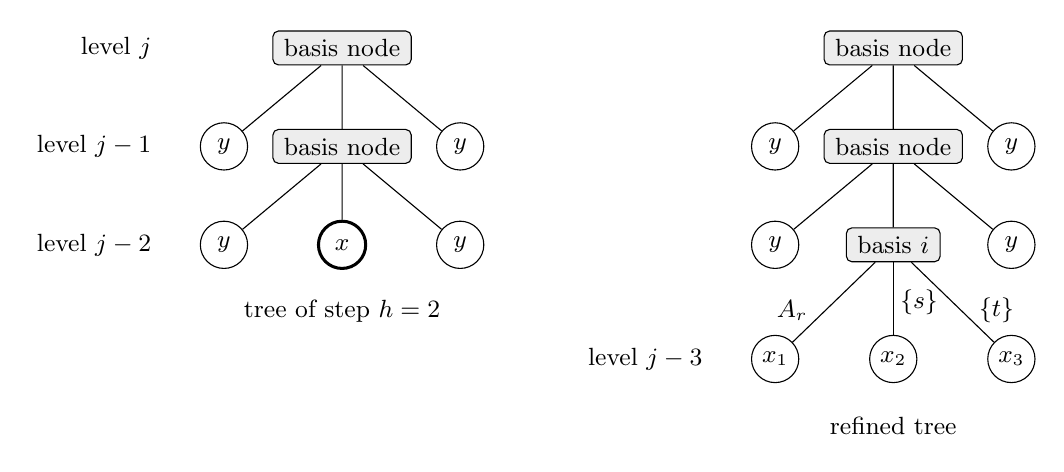
\begin{tikzpicture}[x=1cm,y=1cm,
   inner/.style={draw=black,fill=black!7,rounded corners=2pt,inner xsep=4pt,inner ysep=3pt,font=\small},
   leaf/.style={draw=black,circle,inner sep=1pt,minimum size=6mm,font=\small},
   marked/.style={leaf,line width=1.1pt},
   every node/.style={font=\small}]
\begin{scope}
 \node[inner] (r) at (0,0) {basis node};
 \node[leaf] (r1) at (-1.5,-1.25) {$y$};
 \node[inner] (m) at (0,-1.25) {basis node};
 \node[leaf] (r3) at (1.5,-1.25) {$y$};
 \node[leaf] (m1) at (-1.5,-2.5) {$y$};
 \node[marked] (m2) at (0,-2.5) {$x$};
 \node[leaf] (m3) at (1.5,-2.5) {$y$};
 \draw (r)--(r1) (r)--(m) (r)--(r3) (m)--(m1) (m)--(m2) (m)--(m3);
 \node[anchor=east] at (-2.3,0) {level $j$};
 \node[anchor=east] at (-2.3,-1.25) {level $j-1$};
 \node[anchor=east] at (-2.3,-2.5) {level $j-2$};
 \node at (0,-3.35) {tree of step $h=2$};
\end{scope}
\begin{scope}[xshift=7.0cm]
 \node[inner] (r) at (0,0) {basis node};
 \node[leaf] (r1) at (-1.5,-1.25) {$y$};
 \node[inner] (m) at (0,-1.25) {basis node};
 \node[leaf] (r3) at (1.5,-1.25) {$y$};
 \node[leaf] (m1) at (-1.5,-2.5) {$y$};
 \node[inner] (n) at (0,-2.5) {basis $i$};
 \node[leaf] (m3) at (1.5,-2.5) {$y$};
 \node[leaf] (n1) at (-1.5,-3.95) {$x_1$};
 \node[leaf] (n2) at (0,-3.95) {$x_2$};
 \node[leaf] (n3) at (1.5,-3.95) {$x_3$};
 \draw (r)--(r1) (r)--(m) (r)--(r3) (m)--(m1) (m)--(n) (m)--(m3);
 \draw (n)-- node[left=3pt,pos=.6] {$A_r$} (n1);
 \draw (n)-- node[right=-1pt,pos=.55] {$\{s\}$} (n2);
 \draw (n)-- node[right=3pt,pos=.6] {$\{t\}$} (n3);
 \node[anchor=east] at (-2.3,-3.95) {level $j-3$};
 \node at (0,-4.8) {refined tree};
\end{scope}
\end{tikzpicture}
\caption{The presentation trees in the proof of Theorem~\ref{thm:dimension}, drawn for $h=2$. Left: the tree of step $h$. Its internal nodes are $h$ ternary basis nodes. The marked leaf (bold circle) carries the variable $x$, and the $2h$ side leaves carry the side variable $y$. Right: the refined tree. The marked leaf is replaced by a basis node at a basis $i$, labeled ``basis $i$'', with a ternary template $\{A_r,\{s\},\{t\}\}$; its three children carry independent variables. If the child on $\{s\}$ becomes the marked leaf and the other two children become side leaves, the result is the tree of step $h+1$.}
\label{fig:refinement}
\end{figure}

\begin{proof}[Proof of Theorem~\ref{thm:dimension}]
We construct projections $\Pi_0=I,\Pi_1,\ldots,\Pi_j$ on $\C^d$ such that
\[
 \rank\Pi_{h+1}=\tfrac14\rank\Pi_h\qquad(0\le h\le j-1).
\]
Then $\rank\Pi_j=d/4^j$ is an integer, which proves $4^j\mid d$ for $G_{j,R}$. Each $\Pi_h$ is a coordinate projection~\eqref{eq:coordinate-projection}, and the step from $\Pi_h$ to $\Pi_{h+1}$ recovers the relations of the Mermin--Peres square on the range of $\Pi_h$.

\emph{The tree of step $h$.} All presentation trees in this proof have their root at level $j$, so that they present vertices of $S^j_\lambda(K_3)$. Let $0\le h\le j-1$. The tree of step $h$ has $h$ internal nodes. They are ternary basis nodes at the levels $j,j-1,\ldots,j-h+1$, each a child of the one above it (Figure~\ref{fig:refinement}, left). One leaf, at level $j-h$, is the \emph{marked leaf}; it is a child of the lowest basis node, or the whole tree if $h=0$. The other $2h$ leaves are the \emph{side leaves}. Every leaf is a scalar, padded to the level at which it sits. We assign a variable $x\in\mathbb Z/3$ to the marked leaf and one common variable $y\in\mathbb Z/3$, the \emph{side variable}, to all side leaves. The tree has $h\le2j-1$ internal nodes and no wire node, so it satisfies the bounds of Definition~\ref{def:sparse-graph}. By Fact~1, it defines a graph homomorphism
\[
 F_h:K_3^{\times2}\to G_{j,R},\qquad (y,x)\mapsto F_h(y,x).
\]
The \emph{marked projection} is the coordinate projection of the marked leaf, $\Pi_h=S_{F_h}(\{x\})$. For $h=0$ there are no side leaves, $F_0$ depends only on $x$, and $\Pi_0=I$. The trees of the steps $h\ge1$ are specified at the end of the proof.

\emph{Refining the marked leaf.} Choose a basis $i\in\{1,\ldots,6\}$ and a ternary template $\{A_r,\{s\},\{t\}\}$ at $i$. Replace the marked leaf, which sits at level $j-h\ge1$, by a basis node with this template whose three children are leaves (Figure~\ref{fig:refinement}, right). Assign independent variables $x_1,x_2,x_3\in\mathbb Z/3$ to the children on $A_r$, $\{s\}$ and $\{t\}$, and keep $y$ on the side leaves. The refined tree has $h+1\le j\le2j-1$ internal nodes and no wire node, so by Fact~1 it defines a graph homomorphism $K_3^{\times4}\to G_{j,R}$; for $h=0$ the variable $y$ does not occur. We call the coordinate projections of $x_1,x_2,x_3$ the \emph{child projections} on $A_r$, $\{s\}$ and $\{t\}$. We prove three claims about them and then count ranks.
\begin{list}{}{\setlength{\labelwidth}{3.6em}\setlength{\labelsep}{0.6em}\setlength{\leftmargin}{4.2em}\setlength{\itemsep}{3pt}\setlength{\parsep}{0pt}\setlength{\topsep}{4pt}}
\item[\textup{Claim 1.}] For every basis $i$ and every ternary template at $i$, the three child projections are pairwise orthogonal and sum to $\Pi_h$.
\item[\textup{Claim 2.}] Fix a basis $i$. For $s\in\{1,2,3\}$, the child projection on the singleton $\{s\}$ is the same for the two ternary templates at $i$ that contain $\{s\}$; we denote it by $T^i_s$. With $T^i_0=\Pi_h-T^i_1-T^i_2-T^i_3$, the operators $T^i_0,T^i_1,T^i_2,T^i_3$ are pairwise orthogonal projections with sum $\Pi_h$, and the child projection on $A_r$ is $D^i_r=T^i_0+T^i_r$ for $r=1,2,3$.
\item[\textup{Claim 3.}] Let $e=ik$ be an edge of $K_{3,3}$ with $A_{i,e}=A_r$. If $e\ne36$ and $A_{k,e}=A_{r'}$, then $D^i_r=D^k_{r'}$. For the complemented edge, $D^3_3=\Pi_h-D^6_3$.
\end{list}

\emph{Proof of Claim~1.} The three child projections are pairwise orthogonal by Fact~3. For the sum, set $x_1=x_2=x_3=x$. The refined tree then presents a vertex $F^i_h(y,x)$, in which the marked leaf is replaced by the constant word on $x$ in basis $i$. By Fact~5, the three child projections sum to the coordinate projection of $x$ for the homomorphism $F^i_h$. It therefore suffices to show that
\[
 P_{F^i_h(y,x),a}=P_{F_h(y,x),a}\qquad\text{for all }y,x,a\in\mathbb Z/3\text{ and every basis }i.
\]
For $i=6$ this holds because the constant word on $x$ in basis $6$ is the padding of the scalar $x$, so that $F^6_h=F_h$. Now let $e=ik$ be an edge of $K_{3,3}$. For each layer $\ell\in\{0,\ldots,\lambda+1\}$, replace the marked leaf by a wire node on $e$ at layer $\ell$ whose two children are both the scalar leaf $x$. This tree has $h+1\le2j-1$ internal nodes, one of them a wire node with a scalar background, so it satisfies Definition~\ref{def:sparse-graph}. At the layers $0$ and $\lambda+1$ it presents $F^i_h(y,x)$ and $F^k_h(y,x)$. By Fact~2, the homomorphisms of two consecutive layers satisfy the cross-edge condition, so by Fact~7 they carry the same measurements. Hence so do $F^i_h$ and $F^k_h$. Since $K_{3,3}$ is connected, the measurements of every $F^i_h$ agree with those of $F^6_h=F_h$.

\emph{Proof of Claim~2.} Let $s\in\{1,2,3\}$, and consider one of the two ternary templates at $i$ that contain $\{s\}$. Set the variable of the child on $\{s\}$ equal to $x$ and the variables of the other two children equal to $y$. By Fact~5, this identification leaves the child projection on $\{s\}$ unchanged: it becomes the coordinate projection of $x$ for the resulting homomorphism $K_3^{\times2}\to G_{j,R}$. The vertex that this homomorphism presents has, in place of the marked leaf, the word of basis $i$ with $x$ at position $s$ and $y$ at the other three positions. This word is the same for both templates, so the child projection on $\{s\}$ does not depend on the template. Two distinct positions $s,t\in\{1,2,3\}$ are singleton parts of one template $\{A_r,\{s\},\{t\}\}$. By Claim~1, the projections $T^i_s$ and $T^i_t$ are therefore orthogonal, and both lie below $\Pi_h$. Hence $T^i_0$ is a projection, and $T^i_0,T^i_1,T^i_2,T^i_3$ are pairwise orthogonal with sum $\Pi_h$. Finally, by Claim~1 the child projection on $A_r$ equals $\Pi_h-T^i_s-T^i_t=T^i_0+T^i_r$.

\emph{Proof of Claim~3.} Let $e=ik$ be an edge of $K_{3,3}$ with $i\le3<k$. For each layer $\ell\in\{0,\ldots,\lambda+1\}$, replace the marked leaf by a wire node on $e$ at layer $\ell$ whose first child is a leaf with the variable $x$ and whose background is a leaf with the side variable $y$. As in the proof of Claim~1, these trees satisfy Definition~\ref{def:sparse-graph}. By Facts~2 and~7, the measurements are the same at all layers, and so is the coordinate projection of $x$. At layer $0$ the tree presents the word of basis $i$ with $x$ on $A_{i,e}=A_r$ and $y$ on the complement. As in the proof of Claim~2, the coordinate projection of $x$ is then the child projection on $A_r$ at basis $i$, which is $D^i_r$. At layer $\lambda+1$ the tree presents the word of basis $k$ with $x$ on $A_{k,e}$ and $y$ on the complement. If $e\ne36$ and $A_{k,e}=A_{r'}$, the coordinate projection of $x$ is $D^k_{r'}$ for the same reason. If $e=36$, then $x$ occupies $A_{6,36}=A_3^c=\{1,2\}$ and $y$ occupies $A_3$. For the template $\{A_3,\{1\},\{2\}\}$ this is the word whose two singleton children both carry $x$, so the coordinate projection of $x$ is $T^6_1+T^6_2=\Pi_h-D^6_3$.

\emph{The relations of the square.} By Claim~2, the operators
\[
 L^i_r=2D^i_r-\Pi_h\qquad(r=1,2,3)
\]
are self-adjoint involutions on the range of $\Pi_h$. They commute pairwise and satisfy $L^i_1L^i_2L^i_3=\Pi_h$: on the range of $T^i_0$ all three equal $+1$, and on the range of $T^i_s$ with $s\ge1$ the involution $L^i_r$ equals $+1$ for $r=s$ and $-1$ for $r\ne s$. In particular, the ranges of $T^i_0,T^i_1,T^i_2,T^i_3$ are the four joint eigenspaces of any two of $L^i_1,L^i_2,L^i_3$. By Claim~3, an edge $e=ik$ with $A_{i,e}=A_r$ and $A_{k,e}=A_{r'}$ gives $L^i_r=L^k_{r'}$ if $e\ne36$, and the complemented edge gives $L^3_3=-L^6_3$.

Arrange the nine involutions of the row bases in a $3\times3$ array: for an edge $e=ik$ with $A_{i,e}=A_r$, put $L^i_r$ in row $i\in\{1,2,3\}$ and column $k\in\{4,5,6\}$. Row $i$ consists of $L^i_1,L^i_2,L^i_3$, because the three edges at basis $i$ use $A_1,A_2,A_3$ once each (Table~\ref{tab:edges}). Its entries commute, and their product is $+\Pi_h$. By the relations just stated, column $k\in\{4,5\}$ consists of $L^k_1,L^k_2,L^k_3$, and column $6$ consists of $L^6_1$, $L^6_2$ and $-L^6_3$. Hence the entries of every column commute, columns $4$ and $5$ have product $+\Pi_h$, and column $6$ has product $-\Pi_h$. These are the relations of the array~\eqref{eq:pauli-square}. Negating the two entries of row $1$ in columns $4$ and $5$ leaves all row products equal to $+\Pi_h$ and makes all three column products equal to $-\Pi_h$. Call the resulting array $U$.

\emph{Counting ranks.} Lemma~\ref{lem:square-rank}, applied on the range of $\Pi_h$, shows that the four joint eigenspaces of any two distinct entries in a row or in a column of $U$ have equal dimension. Two entries of row $i$ are $\pm L^i_r$ and $\pm L^i_{r'}$ with $r\ne r'$, and two entries of column $k$ are $\pm L^k_r$ and $\pm L^k_{r'}$ with $r\ne r'$. In both cases the four joint eigenspaces are the ranges of $T^b_0,T^b_1,T^b_2,T^b_3$ for the basis $b$ in question. Therefore, for every basis $i\in\{1,\ldots,6\}$,
\begin{equation}\label{eq:quarter-rank}
 \rank T^i_s=\tfrac14\rank\Pi_h\qquad (0\le s\le3).
\end{equation}

\emph{The next step.} Choose a basis $i$ and a ternary template $\{A_r,\{s\},\{t\}\}$ at $i$, and refine the marked leaf accordingly. In the refined tree, let the child on $\{s\}$ be the new marked leaf, with the variable $x$, and let the children on $A_r$ and $\{t\}$ be side leaves, with the variable $y$. As in the proof of Claim~2, the marked projection of this tree is $T^i_s$. We put $\Pi_{h+1}=T^i_s$, so that $\rank\Pi_{h+1}=\frac14\rank\Pi_h$ by~\eqref{eq:quarter-rank}. If $h+1\le j-1$, this tree is the tree of step $h+1$, and the construction continues. Starting from $\Pi_0=I$, we obtain $\rank\Pi_j=d/4^j$ after $j$ steps, which proves $4^j\mid d$ for $G_{j,R}$.

Because every quantum $3$-coloring of $S^j_\lambda(K_3)$ restricts to the induced subgraph $G_{j,R}$, $4^j\mid d$ also holds for $S^j_\lambda(K_3)$. Conversely, Theorems~\ref{thm:gap} and~\ref{thm:sparse} supply an $R$-compatible quantum $3$-coloring of both graphs in local dimension $4^j$, and taking direct sums produces $R$-compatible quantum $3$-colorings in every positive multiple of $4^j$.
\end{proof}

The magic square game is known to self-test two EPR pairs because its perfect strategies are rigid up to local isometries~\cite{WBMS,CS}. Theorem~\ref{thm:dimension} establishes an analogous rigidity statement for the graph coloring game at the level of local dimension: every quantum $3$-coloring of $G_{j,R}$ or $S^j_\lambda(K_3)$ must embed the algebraic relations of the Mermin--Peres square $j$ times in succession, regardless of compatibility.

\subsection{Exact compatibility radius and proof of the main theorem}\label{sec:largest-radius}

The involutions recovered at step $h=0$, where $\Pi_0=I$, also show that no quantum $3$-coloring of $G_{j,R}$ or $S^j_\lambda(K_3)$ can commute beyond distance $\max\{R,2\}$.

\begin{proposition}\label{prop:largest-compatible-radius}
For all $j,R\ge1$, the largest integer $k$ for which $G_{j,R}$ admits a $k$-compatible quantum $3$-coloring is $\lambda+2=\max\{R,2\}$, where $\lambda=\max\{R-2,0\}$. The same holds for the full iterate $S^j_\lambda(K_3)$.
\end{proposition}
\begin{proof}
By Theorems~\ref{thm:gap} and~\ref{thm:sparse}, the displayed coloring is $(\lambda+2)$-compatible on both $S^j_\lambda(K_3)$ and $G_{j,R}$.

For the upper bound, let $(P_{v,a})$ be an arbitrary finite-dimensional quantum $3$-coloring of $G_{j,R}$ on $\C^d$. Consider step $h=0$ of the proof of Theorem~\ref{thm:dimension}, where $\Pi_0=I$, and its two involutions
\[
 L^1_2=2D^1_2-I,\qquad L^4_1=2D^4_1-I.
\]
By Table~\ref{tab:edges}, $L^1_2$ belongs to the edge $15$ and stands in row $1$ and column $5$ of the array of involutions. By Claim~3 of that proof, $L^4_1=L^2_2$, which belongs to the edge $24$ and stands in row $2$ and column $4$. Up to sign, these are two entries of the array $U$ in distinct rows and distinct columns. Such entries anticommute by Lemma~\ref{lem:square-rank}, and a change of sign does not affect this. Hence $L^1_2L^4_1=-L^4_1L^1_2$.

We recover $D^1_2$ and $D^4_1$ from four concrete vertices of $G_{j,R}$. Write each entry below for a scalar padded to level $j-1$ in basis $6$:
\[
\begin{array}{c|cc}
 &\text{constant word}&\text{two-label word}\\ \hline
 \text{basis }1&r_0=(1,1,1,1)&r_1=(1,0,1,0)\\
 \text{basis }4&c_0=(2,2,2,2)&c_1=(2,2,1,1).
\end{array}
\]
The vertices $r_0,r_1$ belong to the ternary template with doubleton $A_2=\{0,2\}$ in basis $1$, and $c_0,c_1$ belong to the ternary template with doubleton $A_1=\{0,1\}$ in basis $4$. By Fact~4, a coordinate projection may be evaluated using any two distinct color labels (here $1$ and $0$ for $D^1_2$, and $2$ and $1$ for $D^4_1$), yielding
\[
 D^1_2=\sum_{a\in\mathbb Z/3} P_{r_0,a}P_{r_1,a},\qquad
 D^4_1=\sum_{a\in\mathbb Z/3} P_{c_0,a}P_{c_1,a}.
\]

We now bound $\dist_{G_{j,R}}(r_i,c_{i'})$ for all $i,i'\in\{0,1\}$. In basis $1$, both $r_0$ and $r_1$ avoid color $2$ in all four positions, so both are adjacent to the constant word $u_1=(2,2,2,2)$ in basis $1$. Similarly, in basis $4$, both $c_0$ and $c_1$ avoid color $0$ in all four positions, so both are adjacent to the constant word $u_4=(0,0,0,0)$ in basis $4$. Along wire $14$, we join $u_1$ (layer $0$) to $u_4$ (layer $\lambda+1$) by a path of $\lambda+1$ edges. To this end, take any walk $a_0,a_1,\ldots,a_{\lambda+1}$ in $K_3$ of length $\lambda+1$ with $a_0=2$ and $a_{\lambda+1}=0$, and place the equal pair $(a_\ell,a_\ell)$, padded to level $j-1$, at layer $\ell$. Such a walk exists for every $\lambda+1\ge1$: lengths $1$ and $2$ use $2,0$ and $2,1,0$, and any walk extends by two steps via a single backtrack. Every basis word and wire vertex along this path admits a presentation with $1$ internal node and at most $1$ wire node, hence lies in $G_{j,R}$ for every $j\ge1$. Therefore
\[
 \dist_{G_{j,R}}(r_i,c_{i'})\le 1+(\lambda+1)+1=\lambda+3\qquad (i,i'\in\{0,1\}).
\]

If $(P_{v,a})$ were $(\lambda+3)$-compatible, every projector at $r_0$ or $r_1$ would commute with every projector at $c_0$ or $c_1$. Then $D^1_2$ and $D^4_1$, and hence $L^1_2$ and $L^4_1$, would commute. Because $L^1_2$ and $L^4_1$ are involutions on the nonzero space $\C^d$, their product is invertible, which contradicts $L^1_2L^4_1=-L^4_1L^1_2$. Thus no quantum $3$-coloring of $G_{j,R}$ is $(\lambda+3)$-compatible. Finally, because distances in the induced subgraph $G_{j,R}$ are at least distances in the full iterate $S^j_\lambda(K_3)$, any $k$-compatible coloring of $S^j_\lambda(K_3)$ restricts to a $k$-compatible coloring of $G_{j,R}$, proving the same upper bound $\lambda+2$ for $S^j_\lambda(K_3)$.
\end{proof}

For $R\ge2$, Proposition~\ref{prop:largest-compatible-radius} states that the compatibility radius of $G_{j,R}$ and $S^j_\lambda(K_3)$ is exactly $R$: no choice of quantum strategy on these graphs can commute further. When $R\in\{1,2\}$, we have $\lambda=0$, so $G_{j,1}=G_{j,2}$ and their compatibility radius is exactly $2$.

Every ingredient of Theorem~\ref{thm:main} is now established, and we assemble its proof.

\begin{proof}[Proof of Theorem~\ref{thm:main}]
Let $j,R\ge1$, $\lambda=\max\{R-2,0\}$, and $G=S^j_\lambda(K_3)$. Theorem~\ref{thm:gap} establishes $\cq(G)=3$, $\chi(G)\ge2j+3$, and a $(\lambda+2)$-compatible, hence $R$-compatible, quantum $3$-coloring in local dimension $4^j$. As explained in Section~\ref{sec:sparse} using~\eqref{eq:pauli-square}, this strategy consists of adaptive two-qubit Pauli measurements on $2j$ EPR pairs, proving~(i). Theorem~\ref{thm:dimension} proves~(ii), that every finite-dimensional quantum $3$-coloring of $G$ has local dimension divisible by $4^j$, assuming only the edge rule. Proposition~\ref{prop:largest-compatible-radius} proves~(iii), that no quantum $3$-coloring of $G$ is $k$-compatible for any $k>\max\{R,2\}$. Finally, Theorem~\ref{thm:sparse} provides the explicit induced subgraph $G_{j,R}$ of $G$. It satisfies $\cq(G_{j,R})=3$, $\chi(G_{j,R})\ge2j+3$ and $|V(G_{j,R})|+|E(G_{j,R})|\le[C(1+R)]^j$ for an absolute constant $C$, and the adaptive Pauli coloring restricts to an $R$-compatible quantum $3$-coloring of $G_{j,R}$ in local dimension $4^j$. Theorem~\ref{thm:dimension} and Proposition~\ref{prop:largest-compatible-radius} establish~(ii) and~(iii) directly for $G_{j,R}$ as well, which proves~(iv).
\end{proof}

\section{Universal trade-offs: order, compatibility radius, and local dimension}\label{sec:universal}

Sections~\ref{sec:construction}--\ref{sec:rigidity} focused on our explicit family. We now step back and ask what \emph{every} graph with an $R$-compatible quantum $3$-coloring and $\chi(G)\ge t$ must pay in graph order, edge count, and local dimension. We obtain four main results. At fixed $t$, the lower bound on the order that holds for all graphs has the same exponent in $R$ as the order of $G_{j,R}$. Every graph with a quantum $3$-coloring in local dimension three is classically $5$-colorable, and this bound is attained at every compatibility radius. The general exponential upper bound on $\chi(G)$ for quantum $3$-colorings in local dimension $d$ becomes tighter. Finally, lower bounds that are certified by the box complex meet structural barriers.

\subsection{Local classicality and neighborhood rounding}\label{sec:compatibility}

Compatibility is a locality condition. Commuting projective measurements can be performed jointly, and $R$-compatibility requires joint measurability for all pairs of vertices within graph distance $R$~\cite[Section~2.1]{C26}. Whenever a subset $U\subseteq V(G)$ has diameter at most $R$ in $G$, the measurements of an $R$-compatible quantum $3$-coloring on $U$ commute pairwise and therefore admit a common orthonormal eigenbasis. Each vector in this basis selects one color at every vertex of $U$, and the edge rule guarantees that this assignment is a proper classical $3$-coloring of $G[U]$. On every set of diameter at most $R$, an $R$-compatible strategy thus reduces to a probability distribution over proper classical colorings; Ciardo and Mottet accordingly describe highly compatible strategies as locally classical~\cite[Section~3]{CM}. Larger compatibility radii force the quantum advantage to be increasingly global.

Simultaneous diagonalization immediately implies that every set of diameter at most $R$---in particular every ball of radius $\lfloor R/2\rfloor$---induces a classically $3$-colorable subgraph. The next lemma extends classical $3$-colorability outward by one additional layer of neighbors, using only the edge rule.

\begin{lemma}[Rounding a commuting set and its neighbors]\label{lem:rounding-neighbors}
Let $(P_{v,a})$ be a quantum $3$-coloring of a graph $G$, and let $S$ be a nonempty set of vertices whose measurements commute pairwise. Then the subgraph induced by $S$ together with all neighbors of vertices of $S$ is classically $3$-colorable. In particular, if the coloring is $R$-compatible, every ball of radius $\lfloor R/2\rfloor+1$ induces a classically $3$-colorable subgraph.
\end{lemma}
\begin{proof}
Because the measurements on $S$ commute pairwise, they share a common unit eigenvector $\xi\in\C^d$. Set $p_{v,a}=\|P_{v,a}\xi\|^2$ for every $v\in V(G)$ and $a\in\{1,2,3\}$, and write $N[S]$ for the closed neighborhood of $S$ (all vertices of $S$ together with all neighbors of vertices of $S$).

Every $s\in S$ has a unique color $a_s$ with $P_{s,a_s}\xi=\xi$ (so $p_{s,a_s}=1$). For any neighbor $v$ of $s$, the edge rule gives $P_{v,a_s}\xi=P_{v,a_s}P_{s,a_s}\xi=0$. Consequently, every vertex $v\in N[S]$ has at most two outcomes of positive probability under $\xi$. Since these probabilities sum to $1$, at least one outcome at $v$ satisfies $p_{v,a}\ge1/2$.

Whenever $v\in N[S]$ and $a\in\{1,2,3\}$ satisfy $p_{v,a}=1/2$, call $P_{v,a}\xi-\xi/2$ a \emph{tie vector}. Each tie vector is nonzero: expanding its squared norm using $P_{v,a}^2=P_{v,a}$ gives
\[
 \|P_{v,a}\xi-\xi/2\|^2=\|P_{v,a}\xi\|^2-\|P_{v,a}\xi\|^2+\frac14=\frac14\ne0.
\]
Choose a real-linear functional $L:\C^d\to\R$ that is nonzero on each of the finitely many tie vectors. Color each vertex $v\in N[S]$ as follows. If a unique outcome $a$ satisfies $p_{v,a}>1/2$, assign $v$ the color $a$. Otherwise two outcomes $a,b$ satisfy $p_{v,a}=p_{v,b}=1/2$. In that case $P_{v,a}\xi+P_{v,b}\xi=\xi$, so the two tie vectors satisfy $(P_{v,a}\xi-\xi/2)+(P_{v,b}\xi-\xi/2)=0$, and $L$ is positive on exactly one of them. Assign $v$ the color among $\{a,b\}$ whose tie vector satisfies $L>0$.

To verify that this coloring of $G[N[S]]$ is proper, suppose adjacent vertices $u,v\in N[S]$ both receive color $a$. By the edge rule, $P_{u,a}$ and $P_{v,a}$ are orthogonal projections, so $p_{u,a}+p_{v,a}=\|(P_{u,a}+P_{v,a})\xi\|^2\le1$. Since both probabilities are at least $1/2$, we must have $p_{u,a}=p_{v,a}=1/2$ and $\|(P_{u,a}+P_{v,a})\xi\|^2=1$, which forces $(P_{u,a}+P_{v,a})\xi=\xi$. The two tie vectors $P_{u,a}\xi-\xi/2$ and $P_{v,a}\xi-\xi/2$ are therefore opposite, so $L$ cannot be positive on both, a contradiction.

For the final assertion, let $S$ be any ball of radius $\lfloor R/2\rfloor$ in $G$. Any two vertices of $S$ lie at distance at most $2\lfloor R/2\rfloor\le R$, so their measurements commute by $R$-compatibility, and $N[S]$ is the concentric ball of radius $\lfloor R/2\rfloor+1$.
\end{proof}

\subsection{Graph order versus compatibility radius}\label{sec:order}

For integers $t\ge4$ and $R\ge1$, define $N_3(t,R)$ to be the minimum number of vertices of a finite graph $H$ satisfying $\chi(H)\ge t$ that admits an $R$-compatible quantum $3$-coloring (minimized over all graphs, not only those from our construction, and over all finite local dimensions). We first determine the exact asymptotic growth of $N_3(t,R)$ for fixed $t$ as $R\to\infty$.

\begin{corollary}\label{cor:radius}
Put $j=\lceil(t-3)/2\rceil$. For an absolute constant $C$,
\[
 \left\lfloor\frac{R+2}{4j}\right\rfloor^j
 < N_3(t,R) \le [C(1+R)]^j.
\]
In particular, for each fixed $t\ge4$, as $R\to\infty$, $N_3(t,R)=\Theta_t((1+R)^{\lceil(t-3)/2\rceil})$.
\end{corollary}
\begin{proof}
For the upper bound, Theorem~\ref{thm:sparse} produces the graph $G_{j,R}$ with an $R$-compatible quantum $3$-coloring, $\chi(G_{j,R})\ge2j+3\ge t$, and $|V(G_{j,R})|\le[C(1+R)]^j$.

For the lower bound, let $H$ be any $n$-vertex graph with $\chi(H)\ge t$ and an $R$-compatible quantum $3$-coloring, and put $q=\lfloor R/2\rfloor+1$. By Lemma~\ref{lem:rounding-neighbors}, every ball of radius $q$ in $H$ is classically $3$-colorable. The local coloring theorem of Kierstead, Szemer{\'e}di, and Trotter~\cite[Theorem~1]{KST}, in the formulation stated by Bogdanov~\cite[Equation~(1.1)]{BogOrder}, asserts that any graph on at most $\lfloor q/(2j)\rfloor^j$ vertices in which every ball of radius $q$ is $3$-colorable has chromatic number at most $j(3-1)+1=2j+1$. Since $j=\lceil(t-3)/2\rceil$, we have $t\in\{2j+2,2j+3\}$, so $\chi(H)\ge t>2j+1$. Therefore
\[
 n>\left\lfloor\frac{q}{2j}\right\rfloor^j
 =\left\lfloor\frac{\lfloor R/2\rfloor+1}{2j}\right\rfloor^j
 =\left\lfloor\frac{R+2}{4j}\right\rfloor^j
\]
(when the floor is zero, this reduces to $n>0$). Taking the minimum over $H$ proves the displayed inequality, and fixing $t\ge4$ while letting $R\to\infty$ gives $N_3(t,R)=\Theta_t((1+R)^{\lceil(t-3)/2\rceil})$.
\end{proof}

We now turn to the opposite regime: growing classical target $t\to\infty$ at fixed compatibility radius ($R=1$) or at compatibility radius proportional to $t$ ($R\ge\alpha t$). Here we convert any quantum $3$-coloring into a \emph{strict vector $3$-coloring} in the sense of Karger, Motwani, and Sudan~\cite{KMS}. Endow the real vector space of triples $A=(A_1,A_2,A_3)$ of $d\times d$ Hermitian matrices with the inner product $\langle A,B\rangle=\frac1d\sum_{a=1}^3\operatorname{Tr}(A_aB_a)$. For each vertex $v\in V(G)$, define the traceless triple
\begin{equation}\label{eq:strict-vectors}
 x_v=\sqrt{\frac32}\,\bigl(P_{v,a}-\tfrac13 I\bigr)_{a=1}^3.
\end{equation}
Because $P_{v,a}^2=P_{v,a}$ and $\sum_{a=1}^3 P_{v,a}=I$, direct expansion gives
\[
 \|x_v\|^2=\frac{3}{2d}\sum_{a=1}^3\operatorname{Tr}\!\left(P_{v,a}-\frac23 P_{v,a}+\frac19 I\right)
 =\frac{3}{2d}\left(\frac13 d+\frac13 d\right)=1.
\]
On any edge $uv\in E(G)$, the edge rule $P_{u,a}P_{v,a}=0$ gives
\[
 \langle x_u,x_v\rangle=\frac{3}{2d}\sum_{a=1}^3\operatorname{Tr}\!\left(-\frac13 P_{u,a}-\frac13 P_{v,a}+\frac19 I\right)
 =\frac{3}{2d}\left(-\frac13 d\right)=-\frac12.
\]
Thus $(x_v)_{v\in V(G)}$ is a strict vector $3$-coloring of $G$~\cite{KMS}.

\begin{proposition}\label{prop:unrestricted-order}
As $t\to\infty$, one has $N_3(t,1)\ge t^{3+\sqrt6-o(1)}$. For every fixed $\alpha>0$ and $R\ge\alpha t$, one has $N_3(t,R)\ge\exp(\Omega_\alpha(t))$.
\end{proposition}
\begin{proof}
\emph{Fixed radius $R=1$.} Let $G$ be any $n$-vertex graph admitting the strict vector $3$-coloring~\eqref{eq:strict-vectors}, and set $\beta=\sqrt{2/3}$. We lower-bound the independence number of $G$ by splitting on its maximum degree $\Delta(G)$:
\begin{itemize}
\item If $\Delta(G)\le n^\beta$, the vector-coloring theorem of Deguchi, Kawarabayashi, H.~Yoneda, and M.~Yoneda~\cite[Theorem~2]{DKYY} (in its branch $\beta>1/3$) guarantees an independent set of size at least $n^{(2+2\beta)/(2+3\beta)-o(1)}$.
\item If some vertex $v$ has degree greater than $n^\beta$, consider the vectors $y_u=(2x_u+x_v)/\sqrt3$ for all neighbors $u$ of $v$. Using $\|x_u\|=\|x_v\|=1$ and $\langle x_u,x_v\rangle=-1/2$, we compute $\|y_u\|^2=(4-2+1)/3=1$. For any two adjacent neighbors $u,u'$ of $v$, we have $\langle x_u,x_{u'}\rangle=-1/2$ as well, giving $\langle y_u,y_{u'}\rangle=(-2-1-1+1)/3=-1$, so $y_u=-y_{u'}$. Every connected component of the neighborhood of $v$ is therefore bipartite, yielding an independent set of size at least $\deg(v)/2>n^\beta/2$.
\end{itemize}
Because $\beta=\sqrt{2/3}$ solves $(2+2\beta)/(2+3\beta)=\beta$, both branches produce an independent set of size at least $n^{\beta-o(1)}$ as $n\to\infty$.

Since every induced subgraph inherits~\eqref{eq:strict-vectors}, we color $G$ greedily by repeatedly extracting a maximum independent set. Fix any $\varepsilon>0$; there is $m_0(\varepsilon)$ such that every induced subgraph of order $m\ge m_0(\varepsilon)$ has an independent set of size at least $m^{\beta-\varepsilon}$. While the remaining number of vertices lies in $(m/2,m]$ with $m\ge 2m_0(\varepsilon)$, each extracted independent set uses $1$ color and removes at least $(m/2)^{\beta-\varepsilon}$ vertices, so at most $(m/2)/(m/2)^{\beta-\varepsilon}=(m/2)^{1-\beta+\varepsilon}$ colors suffice to halve the graph. Summing this geometric series over dyadic scales $m=n,n/2,n/4,\ldots$ down to $2m_0(\varepsilon)$ and coloring the leftover vertices individually yields $\chi(G)\le O_\varepsilon(n^{1-\beta+\varepsilon})$. Since $\varepsilon>0$ is arbitrary, $\chi(G)\le n^{1-\beta+o(1)}$ as $n\to\infty$. Inverting this bound for $\chi(G)\ge t$ and noting $1/(1-\sqrt{2/3})=3+\sqrt6$ gives $N_3(t,1)\ge t^{3+\sqrt6-o(1)}$ as $t\to\infty$.

\emph{Linear radius $R\ge\alpha t$.} Fix $\alpha>0$ and let $G$ be a graph with $\chi(G)\ge t$ and an $R$-compatible quantum $3$-coloring. Set $r=\min\{\lfloor R/2\rfloor,\lfloor(t-1)/12\rfloor\}$. Since $r\le\lfloor R/2\rfloor+1$, Lemma~\ref{lem:rounding-neighbors} ensures that every ball of radius $r$ in $G$ is classically $3$-colorable. Bogdanov's local coloring theorem~\cite[Theorem~1.1]{BogOrder} applied with $c=3$ and $n=t-1$ implies that $|V(G)|$ is at least a product of $r+1$ rising-factorial terms, each bounded below by $(t-1)/(3(r+1))$, yielding
\[
 |V(G)|\ge \left(\frac{t-1}{3(r+1)}\right)^{r+1}.
\]
Because $r\le(t-1)/12$, for all sufficiently large $t$ the base satisfies $(t-1)/(3(r+1))\ge2$, while $r$ grows at least linearly with $t$ for fixed $\alpha$. Hence $N_3(t,R)\ge 2^{r+1}=\exp(\Omega_\alpha(t))$.
\end{proof}

Combining Theorem~\ref{thm:sparse} (with $j=\lceil(t-3)/2\rceil$) and Proposition~\ref{prop:unrestricted-order} gives
\[
 t^{\,3+\sqrt6-o(1)}\ \le\ N_3(t,1)\ \le\ \exp(O(t))\qquad (t\to\infty),
\]
and for $R$ proportional to $t$ (fixed $\alpha>0$) it gives $\Omega_\alpha(t)\le\log N_3(t,R)\le O_\alpha(t\log t)$. Whether $N_3(t,R)$ can be subexponential in $t$ at a fixed compatibility radius $R$ remains open (Problem~\ref{prob:fixed-radius}). However, the next proposition shows that no graph family whose classical chromatic lower bound is certified by the box complex can have subexponential size.

\begin{proposition}\label{prop:box-barrier}
Let $G$ admit a quantum $3$-coloring. If the box complex $\B(G)$ admits no equivariant map to $S^{t-3}$, where $t\ge3$, then
\[
 |E(G)|\ge(2/\sqrt3)^{t-2},\qquad |V(G)|\ge\sqrt2\,(4/3)^{(t-2)/4}.
\]
\end{proposition}
\begin{proof}
Let $(x_v)_{v\in V(G)}$ be the strict vector $3$-coloring~\eqref{eq:strict-vectors}, and let $W=\operatorname{span}\{x_v:v\in V(G)\}$. Put $m=t-2\ge1$ and form a random linear map $A:W\to\R^m$ whose $m$ rows are independent standard Gaussian vectors in $W$.

Fix one row $g$ of $A$ and one edge $uv\in E(G)$. The Gaussian random variables $X=\langle g,x_u\rangle$ and $Y=\langle g,x_v\rangle$ each have mean $0$, variance $1$, and covariance $\langle x_u,x_v\rangle=-1/2$. Consequently $X+Y$ and $X-Y$ are uncorrelated---hence independent---centered Gaussians with variances $\operatorname{Var}(X+Y)=1+1-1=1$ and $\operatorname{Var}(X-Y)=1+1+1=3$. Using $4XY=(X+Y)^2-(X-Y)^2$ and the standard chi-squared moment generating function $\mathbb E[e^{sZ^2}]=(1-2s)^{-1/2}$ ($s<1/2$, $Z\sim\mathcal N(0,1)$), we compute
\[
 \mathbb E\!\left[e^{2XY/3}\right]
 =\mathbb E\!\left[e^{(X+Y)^2/6}\right]\mathbb E\!\left[e^{-(X-Y)^2/6}\right]
 =\left(1-\frac13\right)^{-1/2}\bigl(1+1\bigr)^{-1/2}=\frac{\sqrt3}{2}.
\]
Since the $m$ rows of $A$ are independent, Markov's inequality bounds the probability of a nonnegative inner product on edge $uv$:
\[
 \Pr\bigl[\langle Ax_u,Ax_v\rangle\ge0\bigr]
 =\Pr\!\left[\exp\!\left(\frac23\langle Ax_u,Ax_v\rangle\right)\ge1\right]
 \le \left(\frac{\sqrt3}{2}\right)^m.
\]

Suppose $|E(G)|(\sqrt3/2)^m<1$. By a union bound over all edges, there exists a realization of $A$ with $\langle Ax_u,Ax_v\rangle<0$ for every edge $uv\in E(G)$. For any point $(\mu,\nu)\in\B(G)$, set $y_\mu=\sum_v \mu(v)Ax_v$ and $y_\nu=\sum_v \nu(v)Ax_v$. Because every $u\in\operatorname{supp}\mu$ is adjacent to every $v\in\operatorname{supp}\nu$, bilinearity gives $\langle y_\mu,y_\nu\rangle=\sum_{u,v}\mu(u)\nu(v)\langle Ax_u,Ax_v\rangle<0$. In particular $\|y_\mu-y_\nu\|^2=\|y_\mu\|^2+\|y_\nu\|^2-2\langle y_\mu,y_\nu\rangle>0$, so $y_\mu\ne y_\nu$. The map
\[
 (\mu,\nu)\longmapsto \frac{y_\mu-y_\nu}{\|y_\mu-y_\nu\|}
\]
is therefore a continuous equivariant map from $\B(G)$ to $S^{m-1}=S^{t-3}$. Contraposition yields $|E(G)|\ge(2/\sqrt3)^{t-2}$. Finally, $2|E(G)|\le|V(G)|(|V(G)|-1)<|V(G)|^2$ gives $|V(G)|\ge\sqrt2\,(4/3)^{(t-2)/4}$.
\end{proof}

In particular, any graph $G$ with a quantum $3$-coloring whose lower bound $\chi(G)\ge t$ is certified by the height of $w$ (or by any obstruction to an equivariant map $\B(G)\to S^{t-3}$) must have exponentially many edges in $t$.

\subsection{Local dimensions up to four}\label{sec:alldim}

For integers $t\ge4$ and $R\ge1$, define $D_3(t,R)$ to be the minimum local dimension of an $R$-compatible quantum $3$-coloring of a graph with $\chi\ge t$, minimized over all graphs and all colorings. Theorem~\ref{thm:sparse} (with $j=\lceil(t-3)/2\rceil$) yields the upper bound $D_3(t,R)\le 4^{\lceil(t-3)/2\rceil}$.

We first pin down quantum $3$-colorings in local dimensions $1,2,3$ completely, at every compatibility radius $R\ge1$.

\begin{theorem}\label{thm:qutrit}
\leavevmode
\begin{enumerate}
\item[(a)] Every graph with a quantum $3$-coloring in local dimension three is classically $5$-colorable. Every graph with a quantum $3$-coloring in local dimension one or two is classically $3$-colorable.
\item[(b)] For every $R\ge1$ there is an explicit graph $Q_R$ on $1080+567\max\{R-2,0\}$ vertices with $\cq(Q_R)=3$, $\chi(Q_R)=5$, and an $R$-compatible quantum $3$-coloring in local dimension three whose compatibility radius is exactly $\max\{R,2\}$.
\end{enumerate}
Consequently $D_3(4,R)=D_3(5,R)=3$ and $D_3(6,R)\ge4$ for every $R\ge1$.
\end{theorem}
\begin{proof}
\emph{Proof of~(a).} First suppose $d\in\{1,2\}$. For each unordered pair of orthogonal $1$-dimensional subspaces (lines) of $\C^d$ that appear as ranges of outcome projectors in the coloring, choose one line from the pair. Call a projector \emph{selected} if it is the identity $I$ or projects onto a chosen line. Because the three projectors at each vertex are orthogonal and sum to $I$ on $\C^d$ ($d\le2$), every vertex has a unique selected projector, and two selected projectors are never orthogonal. Coloring each vertex by the outcome of its selected projector therefore defines a proper $3$-coloring.

Now suppose $(P_{v,a})_{a=1}^3$ is a quantum $3$-coloring of $G$ on $\C^3$. The proof has three steps. Two independent sets $V_1$ and $V_2$ receive the colors $4$ and $5$. In a third independent set $V_3$, a vertex $v$ with $\rank P_{v,3}=2$ receives a mark in $\{1,2\}$ that belongs to the line $\ker P_{v,3}$, and a vertex with $P_{v,3}=I$ receives the color $3$. The remaining vertices, whose three projectors all have rank one, are colored with $1,2,3$ in such a way that each of them avoids the colors of its neighbors in $V_3$ and of its neighbors among the remaining vertices.

Because no two subspaces of $\C^3$ of dimension at least $2$ are orthogonal, the set $V_1=\{v\in V(G):\rank P_{v,1}\ge2\}$ is an independent set, and so is $V_2=\{v\in V(G)\setminus V_1:\rank P_{v,2}\ge2\}$. Assign colors $4$ and $5$ to $V_1$ and $V_2$, respectively. Every remaining vertex $v\in V(G)\setminus(V_1\cup V_2)$ either has $\rank P_{v,3}\ge2$---forming an independent set $V_3$---or is \emph{balanced}, meaning $\rank P_{v,1}=\rank P_{v,2}=\rank P_{v,3}=1$. We color $V_3$ and the balanced vertices using colors $1,2,3$.

Let $\mathcal L$ be the finite set of lines in $\C^3$ occurring either as the range of an outcome projector of a balanced vertex or as $\ker P_{v,3}$ for a vertex $v\in V_3$ with $\rank P_{v,3}=2$. Write $P_\ell$ for the rank-one projection onto $\ell\in\mathcal L$. For each $\ell\in\mathcal L$, the set $\{z\in\C^3:\|z\|=1,\;\|P_\ell z\|^2=1/3\}$ is nowhere dense in the unit sphere of $\C^3$, so we can choose a unit vector $z\in\C^3$ with $\|P_\ell z\|^2\ne1/3$ for every $\ell\in\mathcal L$. Mark each line $\ell\in\mathcal L$ by $f(\ell)=1$ if $\|P_\ell z\|^2<1/3$ and $f(\ell)=2$ if $\|P_\ell z\|^2>1/3$. For any orthonormal basis $\{\ell_1,\ell_2,\ell_3\}\subseteq\mathcal L$, the three weights $\|P_{\ell_r}z\|^2$ sum to $1$ and none equals $1/3$, so not all three can lie on the same side of $1/3$; hence every orthonormal basis in $\mathcal L$ carries both marks $1$ and $2$.

Color every vertex $v\in V_3$ by $f(\ker P_{v,3})$ if $\rank P_{v,3}=2$, and by color $3$ if $P_{v,3}=I$. Note that if a balanced vertex $u$ is adjacent to $v\in V_3$, the edge rule $P_{u,3}P_{v,3}=0$ places the line of $P_{u,3}$ inside $\ker P_{v,3}$; this is impossible when $P_{v,3}=I$, so necessarily $\rank P_{v,3}=2$ and $\ker P_{v,3}$ equals the third line $\operatorname{ran} P_{u,3}$ of $u$.

Consider now the balanced vertices. By~\cite[Lemma~2]{Ji}, any two adjacent balanced vertices $u,u'$ have commuting measurements, so their three rank-one projectors must share the same orthonormal basis $\{m_1,m_2,m_3\}$ of $\C^3$, assigned to outcomes $1,2,3$ by two bijections that disagree at every outcome. Fix an orthonormal basis $\{m_1,m_2,m_3\}\subseteq\mathcal L$. Two bijections $\{1,2,3\}\to\{m_1,m_2,m_3\}$ that disagree at every outcome differ by a $3$-cycle (even permutation), so the six bijections partition into two classes of three, and edges between balanced vertices occur only between distinct bijections inside the same class. Within each class of three bijections, the three third lines (images of outcome $3$) are $m_1,m_2,m_3$, which carry both marks $1$ and $2$:
\begin{itemize}
\item If one of the three bijections has third line of mark $2$ and the other two have third lines of mark $1$, color the first bijection $1$ and the other two bijections $2$ and $3$.
\item If one bijection has third line of mark $1$ and the other two have third lines of mark $2$, color the first bijection $2$ and the other two bijections $1$ and $3$.
\end{itemize}
Assign every balanced vertex the color of its bijection. Inside each class of three bijections, distinct bijections receive distinct colors, so adjacent balanced vertices have different colors. Furthermore, by construction, every balanced vertex receives a color strictly different from the mark $f(\operatorname{ran} P_{u,3})$ of its third line, which is the color of every neighbor of $u$ in $V_3$. Since $V_3$ itself is independent, colors $1,2,3$ properly color $V_3$ together with all balanced vertices, completing a proper $5$-coloring of $G$.

\emph{Proof of~(b).} We apply Proposition~\ref{prop:one-in-three} to Peres' Kochen--Specker configuration in $\R^3$~\cite{Peres91}. Peres' $33$ rays are the lines spanned by all coordinate permutations and sign changes of $(0,0,1)$, $(0,1,1)$, $(0,1,\sqrt2)$, and $(1,1,\sqrt2)$. Among these $33$ rays lie $16$ orthogonal triples (triads) and $24$ additional orthogonal pairs not contained in any of those $16$ triads. Adjoining the common perpendicular of each of these $24$ pairs produces $24$ new lines, yielding $33+24=57$ lines organized into $16+24=40$ orthogonal triads. Let $\mathcal D$ be the set of $40$ triads of rank-one projections onto these lines in $\C^3$, and define
\[
 Q_R=W_\lambda(\mathcal D),\qquad \lambda=\max\{R-2,0\},
\]
fixing arbitrary orderings of the triads containing each line in the definition of $W_\lambda(\mathcal D)$ (Section~\ref{sec:one-in-three}).

Because no two rank-one projections in $\C^3$ are complementary, two parts of different triads in $\mathcal D$ are never complementary, and they are equal precisely when they project onto the same line. A one-in-three selection for $\mathcal D$ would therefore be a subset of the $57$ lines meeting each of the $40$ triads in exactly one line; its restriction to Peres' $33$ rays would meet every one of the $16$ ray triads in exactly one ray and every one of the $24$ orthogonal pairs in at most one ray. Peres proved that no such selection exists~\cite{Peres91}. Hence $\mathcal D$ admits no one-in-three selection.

By Proposition~\ref{prop:one-in-three}, $Q_R$ has a $(\lambda+2)$-compatible, hence $R$-compatible, quantum $3$-coloring in local dimension three, $\cq(Q_R)=3$, and $\chi(Q_R)\ge5$. Part~(a) gives $\chi(Q_R)\le5$, so $\chi(Q_R)=5$. Finally, $Q_R$ has $40$ triad charts of $27$ words each ($40\cdot27=1080$ chart vertices). Across all $40$ triads there are $3\cdot40=120$ part incidences distributed among $57$ distinct lines; connecting the first triad on each line to every other triad sharing that line creates $120-57=63$ wires, each contributing $9\lambda$ interior vertices ($63\cdot9=567$). Thus $|V(Q_R)|=1080+567\max\{R-2,0\}$.

\emph{Compatibility radius of this coloring.} The coloring is $(\lambda+2)$-compatible by Proposition~\ref{prop:one-in-three}. We exhibit two vertices at distance at most $\lambda+3$ whose measurements do not commute. Since $120>57$, some line lies in at least two triads. Let $T_1=\{P,A,B\}$ be the first triad containing it and $T=\{P,A',B'\}$ another one, with $P$ the projection onto that line, so that a wire joins the charts of $T_1$ and $T$. Two distinct triads of rank-one projections on $\C^3$ share at most one part, because two of the three lines determine the third. Hence $A'$ is a rank-one projection below $I-P=A+B$ that differs from both $A$ and $B$. It is therefore neither equal nor orthogonal to $A$, and $AA'\ne A'A$.

With the colors in $\mathbb Z/3$, let $w_1$ be the word of $T_1$ with colors $0,1,2$ on $P,A,B$, and let $w_2$ be the word of $T$ with colors $\lambda+1,\lambda+2,\lambda$ on $P,A',B'$. For $0\le\ell\le\lambda+1$, let $u_\ell$ be the pair $(\ell+1,\ell)$ in layer $\ell$ of the wire. The vertex $u_0$ is the word of $T_1$ with color $1$ on $P$ and $0$ on $A$ and $B$, which differs from $w_1$ on all three parts. Consecutive pairs $u_\ell,u_{\ell+1}$ differ in both entries. The vertex $u_{\lambda+1}$ is the word of $T$ with color $\lambda+2$ on $P$ and $\lambda+1$ on $A'$ and $B'$, which differs from $w_2$ on all three parts. Thus $w_1,u_0,\ldots,u_{\lambda+1},w_2$ is a walk with $\lambda+3$ edges. The measurement of $w_1$ contains the projector $A$ and that of $w_2$ contains $A'$, so the coloring is not $(\lambda+3)$-compatible.

\emph{Derivation of the consequence.} By part~(a), no graph with $\chi\ge4$ admits a quantum $3$-coloring in local dimension $1$ or $2$, so $D_3(4,R)\ge3$, and no graph with $\chi\ge6$ admits one in local dimension at most $3$, so $D_3(6,R)\ge4$. Conversely, for every $R\ge1$, the graph $Q_R$ of part~(b) witnesses $D_3(5,R)\le3$, and $D_3(4,R)\le D_3(5,R)$ directly from the definition of $D_3$. Hence $D_3(4,R)=D_3(5,R)=3$ and $D_3(6,R)\ge4$.
\end{proof}

Ciardo previously proved existentially that graphs admitting a quantum $3$-coloring in local dimension three can satisfy $\chi\ge5$~\cite[Corollary~35 and Example~36]{Ciardo24}; Theorem~\ref{thm:qutrit} provides explicit graphs $Q_R$ at every compatibility radius $R$ and proves that five classical colors is sharp for quantum $3$-colorings in local dimension three.
For graphs admitting a quantum $3$-coloring in local dimension four, a short complementary-plane argument caps the classical chromatic number at six.

\begin{proposition}\label{prop:dim-four}
Every graph with a quantum $3$-coloring in local dimension four is classically $6$-colorable. Hence $D_3(7,R)\ge5$ for every $R$.
\end{proposition}
\begin{proof}
At every vertex $v$, the ranks of the three outcome projectors sum to $4$, so at least one outcome $a(v)\in\{1,2,3\}$ satisfies $\rank P_{v,a(v)}\ge2$; fix one such outcome $a(v)$. Partition the $2$-dimensional subspaces (planes) of $\C^4$ that appear as $\operatorname{ran} P_{v,a(v)}$ into orthogonal complementary pairs $\{W,W^\perp\}$, and assign opposite bits $0$ and $1$ to the two members of each pair. Color $v$ by the pair $(a(v),b(v))\in\{1,2,3\}\times\{0,1\}$, where $b(v)$ is the assigned bit if $\rank P_{v,a(v)}=2$ and $b(v)=0$ if $\rank P_{v,a(v)}\ge3$. If adjacent vertices $u,v$ received the same outcome $a(u)=a(v)$, then $\operatorname{ran} P_{u,a(u)}$ and $\operatorname{ran} P_{v,a(v)}$ would be orthogonal subspaces of $\C^4$ of dimension at least $2$; they must therefore be complementary planes and hence carry opposite bits $b(u)\ne b(v)$. Thus these six colors properly color the graph.
\end{proof}

\subsection{A chromatic bound in every local dimension}\label{sec:rounding}

In any quantum $3$-coloring in local dimension $d$, every vertex still has an outcome projector of rank at least $s=\lceil d/3\rceil$. To convert that large-rank outcome into a classical color, say that a unit vector $z\in\C^d$ \emph{hits} a subspace (or its orthogonal projection $Q$) if $\langle z,Qz\rangle>1/2$, meaning that more than half of its squared norm lies in the subspace. Because $\langle z,Qz\rangle+\langle z,Q'z\rangle\le\|z\|^2=1$ for orthogonal projections $Q,Q'$, a single unit vector cannot hit two orthogonal subspaces.

\begin{theorem}\label{thm:rank-rounding}
There is an absolute constant $C$ such that every graph $G$ with a quantum $3$-coloring in local dimension $d$ satisfies
\[
 \chi(G)\le C\,d^4\left(\frac{2^{5/3}}{3}\right)^d,\qquad \frac{2^{5/3}}{3}=1.0583\ldots
\]
No compatibility is assumed beyond the edge rule.
\end{theorem}

The analytical proof of Theorem~\ref{thm:rank-rounding} constructs a finite hitting set of unit vectors via an operator-norm net and a beta-tail bound, and is given in Appendix~\ref{app:rounding}.

Banakh, Ciardo, Kozik, and Tu{\l}owiecki proved $\chi(G)\le 3(2+o(1))^{d-1}$ for every graph $G$ admitting a quantum $3$-coloring in local dimension $d$~\cite[Theorem~29]{BCKT} (their theorem assumes commutation on edges, which is automatic for three colors by~\cite[Lemma~2]{Ji}). Theorem~\ref{thm:rank-rounding} reduces the exponential base from $2$ to $2^{5/3}/3\approx1.0583$. Inverting~\cite[Theorem~29]{BCKT} gives $D_3(t,R)\ge(1-o(1))\log_2 t$, whereas inverting Theorem~\ref{thm:rank-rounding} gives
\begin{equation}\label{eq:dimension-lower}
 D_3(t,R)\ \ge\ \frac{\log t-O(\log\log t)}{\log(2^{5/3}/3)}
 \ =\ (12.23\ldots-o(1))\,\log_2 t\qquad (t\to\infty),
\end{equation}
uniformly in $R\ge1$. To verify~\eqref{eq:dimension-lower}, put $\theta=3/2^{5/3}$ and suppose a graph with $\chi\ge t$ has a quantum $3$-coloring in local dimension $d$. Taking logarithms in Theorem~\ref{thm:rank-rounding} gives $\log t\le \log C+4\log d+d\log(1/\theta)$. If $d\le\log t/\log(1/\theta)$, then $\log d\le\log\log t+O(1)$, so $d\log(1/\theta)\ge\log t-4\log\log t-O(1)$; larger values of $d$ satisfy this inequality automatically.

\subsection{Box-complex certificates need even local dimension}\label{sec:coexist}

Finally, the local dimension of a quantum $3$-coloring directly constrains the height of the Stiefel--Whitney class $w$ on the box complex $\B(G)$.

\begin{proposition}\label{prop:height-dimension}
Let $G$ have a quantum $3$-coloring in local dimension $d=2^\nu m$ with $m$ odd. Then $w^{2^{\nu+1}}=0$ on the box complex of $G$. In particular, a quantum $3$-coloring in odd local dimension forces $w^2=0$, and $w^2\ne0$ forces every quantum $3$-coloring of $G$ to have even local dimension. If $d$ is odd, there is moreover an equivariant map from $\B(G)$ to the circle $S^1$ with the antipodal involution.
\end{proposition}
\begin{proof}
Let $(P_{v,a})_{a\in\mathbb Z/3}$ be the quantum $3$-coloring, let $\omega=e^{2\pi i/3}$, and define the unitary operator $U_v=\sum_{a\in\mathbb Z/3}\omega^a P_{v,a}$ at each vertex $v\in V(G)$. On any edge $vv'\in E(G)$, the measurements at $v$ and $v'$ commute by~\cite[Lemma~2]{Ji} and equal outcomes are orthogonal. Every joint eigenvalue of $U_v^*U_{v'}$ is therefore $\omega$ or $\omega^2$; since $\omega+\omega^2=-1$, we have $U_v^*U_{v'}+U_{v'}^*U_v=-I$.

For any point $(\mu,\nu)\in\B(G)$, set $A=\sum_v \mu(v)U_v$ and $D=\sum_v \nu(v)U_v$. Because every $v\in\operatorname{supp}\mu$ is adjacent to every $v'\in\operatorname{supp}\nu$ and $\sum_v \mu(v)=\sum_{v'}\nu(v')=1$, we compute
\[
 (A-D)^*(A-D)=A^*A+D^*D-\sum_{v,v'}\mu(v)\nu(v')\bigl(U_v^*U_{v'}+U_{v'}^*U_v\bigr)=A^*A+D^*D+I.
\]
The right-hand side is strictly positive definite, so $\Theta(\mu,\nu)=A-D$ is an invertible $d\times d$ complex matrix depending continuously on $(\mu,\nu)$ and satisfying $\Theta(\nu,\mu)=-\Theta(\mu,\nu)$.

When $d$ is odd, $\det(-\Theta)=-\det\Theta$, so $(\mu,\nu)\mapsto\det\Theta(\mu,\nu)/|\det\Theta(\mu,\nu)|$ is an equivariant continuous map from $\B(G)$ to $S^1$ with the antipodal involution. Pulling back from $\mathbb{RP}^1$ gives $w^2=0$ because $H^2(\mathbb{RP}^1;\Ftwo)=0$.

For general $d=2^\nu m$, let $\ell$ be the real line bundle over the quotient $\B(G)/\{1,T\}$ associated with the double cover, so $w=w_1(\ell)$~\cite{MS}. Any continuous odd map $\B(G)\to W$ into a real vector space $W$ defines a section of $\ell\otimes W$. Viewing $\C^d$ as $\R^{2d}$, the $d$ columns of $\Theta(\mu,\nu)$ together with their multiples by $i$ form $2d$ continuous odd maps to $\R^{2d}$ that are $\R$-linearly independent at every point (because $\Theta(\mu,\nu)$ is invertible over $\C$). They therefore yield a global trivialization of the direct sum $\ell^{\oplus 2d}$, so its total Stiefel--Whitney class equals $1$. By the Whitney product formula~\cite{MS}, working in mod-$2$ cohomology where $(1+w)^{2^{\nu+1}}=1+w^{2^{\nu+1}}$, we obtain
\[
 1=(1+w)^{2d}=(1+w^2)^d=(1+w^{2^{\nu+1}})^m.
\]
The degree-$2^{\nu+1}$ term on the right is $m\,w^{2^{\nu+1}}$, and since $m$ is odd this forces $w^{2^{\nu+1}}=0$. Setting $\nu=0$ gives the two special cases.
\end{proof}

Proposition~\ref{prop:height-dimension} separates two mechanisms for chromatic gaps. The $165$-vertex graph $F_{\rm phys}$ of Section~\ref{sec:165} satisfies $w^3\ne0$ (Theorem~\ref{thm:finite-square}), so Proposition~\ref{prop:height-dimension} forces every quantum $3$-coloring of $F_{\rm phys}$ to have even local dimension, and Theorem~\ref{thm:qutrit}(a) rules out local dimension two, pinning its minimum local dimension at four. Conversely, the qutrit graphs $Q_R$ of Theorem~\ref{thm:qutrit}(b) have quantum $3$-colorings in local dimension three, so, by Proposition~\ref{prop:height-dimension}, $w^2=0$ on $\B(Q_R)$ and $\B(Q_R)$ maps equivariantly to $S^1$. Their fifth color comes from the Kochen--Specker obstruction of Peres' rays and is invisible to the box complex, and they carry no tower of length one (cf.\ Section~\ref{sec:no-seed}). In the opposite direction, whenever $G$ admits a quantum $3$-coloring in local dimension $d$ and its bound $\chi(G)\ge k+2$ is certified by $w^k\ne0$, Proposition~\ref{prop:height-dimension} forces the largest power of two dividing $d$ to satisfy $2^\nu>k/2$.

Summarizing our bounds on $D_3(t,R)$, for every compatibility parameter $R\ge1$:
\[
 D_3(4,R)=D_3(5,R)=3,\qquad 4\le D_3(6,R)\le D_3(7,R)\le16,\qquad D_3(7,R)\ge5,
\]
while for general $t\ge4$, $D_3(t,R)$ lies between~\eqref{eq:dimension-lower} and $4^{\lceil(t-3)/2\rceil}$.

\section{Small witnesses for four and five classical colors}\label{sec:finite}

For the first level of the square substitution, $S_\lambda(K_3)$ of Theorem~\ref{thm:one-level} has $342+81\lambda$ vertices: six basis charts of $57$ words plus $\lambda$ interior layers of $9$ vertices on each of the nine wires. When only $1$-compatibility is required, substantially smaller graphs already witness the first two gaps $(\cq,\chi)=(3,4)$ and $(\cq,\chi)=(3,5)$. In this section we exhibit the smallest known explicit witnesses for these gaps---graphs on $22$ and $165$ vertices---determine which of them can serve as a starting graph for the iterated substitution, and lift Lalonde's $15$-vertex lower bound on $N_3(4,1)$ to a new lower bound $N_3(5,1)\ge21$.

\subsection{Four classical colors on \texorpdfstring{$22$}{22} vertices}\label{sec:f22}

\begin{proposition}\label{prop:twentytwo}
There is a graph $F_{22}$ on $22$ vertices and $42$ edges with $\cq=3$ and $\chi=4$. Every quantum $3$-coloring of $F_{22}$ has local dimension divisible by four, and there is one in local dimension four.
\end{proposition}
\begin{proof}
Construct $F_{22}$ as follows. Take a \emph{center} vertex $o$ adjacent to nine \emph{terminals} $A,\bar A,B,\bar B,C,\bar C,X,Y,Z$, and add the three edges $A\bar A$, $B\bar B$, and $C\bar C$ joining each barred terminal to its unbarred partner. For each of the six entries in the table below, introduce a new \emph{private edge} $uv$, joining $u$ to the indicated left pair of terminals and $v$ to the indicated right pair:
\[
\begin{array}{cc|cc|cc}
\text{left}&\text{right}&\text{left}&\text{right}&\text{left}&\text{right}\\ \hline
 A,X&Z,\bar C & X,B&Y,\bar C & A,Y&B,Z\\
 \bar A,X&C,Z & X,\bar B&Y,C & \bar A,Y&\bar B,Z
\end{array}
\]
This yields $1+9+12=22$ vertices and $9+3+6\cdot5=42$ edges.

\emph{Classical chromatic number $\chi(F_{22})=4$.} Suppose $F_{22}$ had a proper classical $3$-coloring. Because all nine terminals are adjacent to $o$, they use only the two colors different from the color of $o$; encode those two colors as bits in $\{0,1\}$. Since $A\bar A,B\bar B,C\bar C$ are edges, each barred terminal carries the complement of its partner's bit. On any private edge $uv$, if both $u$ and $v$ saw unequal terminal bits on their attached pairs, then both $u$ and $v$ would be forced to take the color of $o$, violating the edge $uv$. Thus every private edge forbids simultaneous disagreement on its left and right pairs. Checking the two rows in the first column pair of the table: if $A=X$ (so $\bar A\ne X$), the second row forces $C=Z$; if $A\ne X$, the first row forces $Z=\bar C$, i.e., $C\ne Z$. Together these give $A\oplus X=C\oplus Z$. By the same check on the second and third column pairs,
\[
 A\oplus X=C\oplus Z,\qquad X\oplus B=Y\oplus C,\qquad A\oplus Y=1\oplus B\oplus Z.
\]
Summing all three equations modulo $2$ cancels every terminal bit and yields $0=1$, a contradiction. Conversely, $4$ colors suffice: color the unbarred terminals with color $1$, the barred terminals with color $2$, the center $o$ and all left private endpoints $u$ with color $3$, and all right private endpoints $v$ with color $4$. Hence $\chi(F_{22})=4$.

\emph{Quantum $3$-coloring in local dimension four.} Write $x,y,z$ in lower case for the single-qubit Pauli matrices (to distinguish them from the terminals $X,Y,Z$). Assign to the six unbarred terminals the two-qubit observables
\[
\begin{array}{lll}
 A=I\otimes z,& B=x\otimes x,& C=z\otimes x,\\
 X=x\otimes I,& Y=z\otimes I,& Z=y\otimes y,
\end{array}
\]
and assign to each barred terminal $\bar S$ the negated observable $-S$. The two observables in every left or right pair of the table commute, and they satisfy the hexagon relations
\[
 AX=CZ,\qquad XB=YC,\qquad AY=-BZ
\]
(Figure~\ref{fig:hexagon}). Color the center $o$ deterministically with outcome $0$ ($P_{o,0}=I$). At each terminal with observable $S$, return outcome $1$ on its $+1$ eigenspace $(I+S)/2$ and outcome $2$ on its $-1$ eigenspace $(I-S)/2$. At each private-edge endpoint attached to commuting terminal observables $U,V$, assign outcomes $0,1,2$ to the three pairwise orthogonal projectors
\[
 \frac{I-UV}{2},\qquad \frac{(I-U)(I-V)}{4},\qquad \frac{(I+U)(I+V)}{4},
\]
which sum to $I$. Outcome $1$ lies inside the $-1$ eigenspaces of both $U$ and $V$ (avoiding their outcome $1$), and outcome $2$ lies inside the $+1$ eigenspaces of both $U$ and $V$ (avoiding their outcome $2$), satisfying all terminal-to-endpoint edges. Across every private edge $uv$, write $U,V$ for the two terminal observables attached to $u$ and $U',V'$ for those attached to $v$. The products $UV$ and $U'V'$ are negatives of each other, by the hexagon relations and the signs of the barred terminals. Thus the outcome-$0$ projectors $(I-UV)/2$ at $u$ and $(I-U'V')/2=(I+UV)/2$ at $v$ are orthogonal. The projectors of the outcomes $1$ and $2$ lie in the range of $(I+UV)/2$ at $u$ and in the range of $(I-UV)/2$ at $v$, so they are orthogonal as well. Every edge rule therefore holds.

The vertices $o,A,\bar A$ form a triangle, so $\cq(F_{22})=3$. Finally, Proposition~\ref{prop:small-dimension} in Appendix~\ref{app:small-dimension} proves that every finite-dimensional quantum $3$-coloring of $F_{22}$ has local dimension divisible by four.
\end{proof}

\begin{figure}[htbp]
\centering
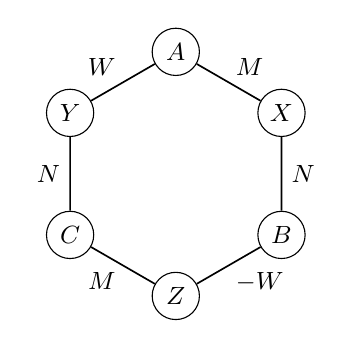
\begin{tikzpicture}[x=1cm,y=1cm,
   point/.style={circle,draw=black,fill=white,inner sep=1.5pt,minimum size=6mm,font=\small},
   every node/.style={font=\small}]
\foreach \name/\angle in {A/90,X/30,B/-30,Z/-90,C/-150,Y/150}
  \node[point] (\name) at (\angle:1.55) {$\name$};
\draw[semithick] (A) -- node[above right=-1pt] {$M$} (X) -- node[right] {$N$} (B)
 -- node[below right=-1pt] {$-W$} (Z) -- node[below left=-1pt] {$M$} (C)
 -- node[left] {$N$} (Y) -- node[above left=-1pt] {$W$} (A);
\end{tikzpicture}
\caption{The six tested pairs of terminals in $F_{22}$ form the edges of a hexagon. In the two-qubit strategy of Proposition~\ref{prop:twentytwo}, each edge carries the product of its two commuting observables, with $M=AX=CZ$, $N=XB=YC$, and $W=AY=-BZ$. No assignment of signs $\pm1$ to the six terminals satisfies these three relations. The six edge values would multiply to $+1$, because every terminal lies on two edges; but the relations give them the form $\varepsilon_1,\varepsilon_2,-\varepsilon_3,\varepsilon_1,\varepsilon_2,\varepsilon_3$ with $\varepsilon_1,\varepsilon_2,\varepsilon_3\in\{\pm1\}$, whose product is $-1$.}
\label{fig:hexagon}
\end{figure}

\subsection{Five classical colors on \texorpdfstring{$165$}{165} measurements}\label{sec:165}

We now trim the physical graph of $S_0(K_3)$ down to $165$ projective measurements that still require five classical colors and still carry a tower of length one. Identify the three colors with $C=\mathbb Z/3$. Call the positions $1,2,3$ of a basis of the square its \emph{tail positions}, and index them by $i\in C$ in order. In each of the six bases, retain the words
\begin{equation}\label{eq:finite-words}
 (k,\,k+p_0,\,k+p_1,\,k+p_2),\qquad
 k\in C,\quad
 p\in\{O,\alpha_i,\beta_i,\delta_i,\upsilon_i:i\in C\},
\end{equation}
where $O=(0,0,0)$, $\alpha_i=\mathbf 1-e_i$ (having $0$ in coordinate $i$ and $1$ in the other two coordinates), $\beta_i=-\alpha_i$, $\delta_i=-e_i$, and $(\upsilon_i)_s=s-i$ for $s\in C$. Notice that each of the $13$ difference triples $p$ has at least one zero coordinate, so every retained word repeats its first letter $k$ and belongs to the $57$ words of Section~\ref{sec:example}; there are $3\cdot13=39$ words per basis.

Assign to each word the three-outcome projective measurement in its basis that maps each ray to its indicated color, and identify equal measurements across bases:
\begin{itemize}
\item For $p=O$, all six bases share the $3$ constant measurements, which we call \emph{scalar} (matching the scalar projectors of Section~\ref{sec:substitution}).
\item For $p\in\{\alpha_i,\beta_i:i\in C\}$, each word takes one color on a shared plane $P_e$ and a second color on $I-P_e$, giving $6$ nonconstant measurements on each of the $9$ planes of~\eqref{eq:planes} ($9\cdot6=54$ measurements).
\item For $p\in\{\delta_i,\upsilon_i:i\in C\}$, each word has a color that occurs at a single ray (a rank-one outcome); because all $24$ basis rays of the square are distinct, these contribute $6\cdot(3\cdot6)=108$ distinct measurements.
\end{itemize}
In total, \eqref{eq:finite-words} yields $3+54+108=165$ distinct projective measurements on $\C^4$. Let $F_{\rm phys}$ be the physical graph on these $165$ measurements, joining two measurements $M,N$ whenever $M_aN_a=0$ for all $a\in C$. Its edge count is $843$ (computed by \texttt{checks/check\_square\_graphs.py}).

\begin{theorem}\label{thm:finite-square}
The graph $F_{\rm phys}$ satisfies $(\cq,\chi)=(3,5)$. There is a tower of length one over $F_{\rm phys}$, so that $w^3\ne0$ on its box complex. The graph has a quantum $3$-coloring in local dimension four and none in a smaller local dimension.
\end{theorem}
\begin{proof}
Appendix~\ref{app:finite} constructs an explicit tower of length one over $F_{\rm phys}$. Applying Proposition~\ref{prop:tower-bound} with $h=1$ immediately gives $w^3\ne0$ on $\B(F_{\rm phys})$ and $\chi(F_{\rm phys})\ge5$. Because $F_{\rm phys}$ is a subgraph of the physical graph of all three-label measurements in the six bases, Proposition~\ref{prop:physical-upper} in Appendix~\ref{app:five-coloring} (with $n=3$) gives $\chi(F_{\rm phys})\le5$; hence $\chi(F_{\rm phys})=5$.

Assigning each vertex of $F_{\rm phys}$ to its own projective measurement gives a quantum $3$-coloring in local dimension four, and the three scalar measurements form a triangle, so $\cq(F_{\rm phys})=3$. Finally, because $w^3\ne0$ implies $w^2\ne0$, Proposition~\ref{prop:height-dimension} excludes every odd local dimension (in particular $d=1$ and $d=3$), while Theorem~\ref{thm:qutrit}(a) excludes local dimension $d=2$ since $\chi(F_{\rm phys})>3$. Thus $F_{\rm phys}$ admits no quantum $3$-coloring in local dimension less than four.
\end{proof}

\subsection{Starting graphs for the iteration}\label{sec:no-seed}

Because $F_{\rm phys}$ carries a tower of length one, it can serve as a starting graph for the square substitution, saving one iteration relative to starting from $K_3$.

\begin{corollary}\label{cor:seed}
For all $j\ge1$ and $\lambda\ge0$, the graph $S^{j-1}_\lambda(F_{\rm phys})$ has quantum chromatic number three, with a quantum $3$-coloring in local dimension $4^j$, and classical chromatic number at least $2j+3$.
\end{corollary}
\begin{proof}
Applying Theorem~\ref{thm:step} with $h=1$ to the tower of length one over $F_{\rm phys}$ from Theorem~\ref{thm:finite-square} gives $\chi(S^{j-1}_\lambda(F_{\rm phys}))\ge 2(1+(j-1))+3=2j+3$. Starting from the identity quantum $3$-coloring of $F_{\rm phys}$ in local dimension four and applying~\eqref{eq:strategy} $j-1$ times produces a quantum $3$-coloring of $S^{j-1}_\lambda(F_{\rm phys})$ in local dimension $4^j$. The constant words on the three scalar measurements form a triangle at every level, so $\cq(S^{j-1}_\lambda(F_{\rm phys}))=3$.
\end{proof}

Corollary~\ref{cor:seed} claims no compatibility beyond the edge rule and no bound on the order. By contrast, a graph with $\chi=4$ can never carry a tower of length one, because Proposition~\ref{prop:tower-bound} forces $w^3\ne0$ and $\chi\ge5$. For $F_{22}$, even $w^2$ vanishes on $\B(F_{22})$.

\begin{proposition}\label{prop:no-seed}
There is an equivariant map from $\B(F_{22})$ to the circle $S^1$ with the antipodal involution. Consequently $w^2=0$ on the box complex of $F_{22}$, there is no tower of length one over $F_{22}$, and the bound~\eqref{eq:classical-obstruction} certifies only three of its four colors.
\end{proposition}
\begin{proof}
Use the proper $4$-coloring of $F_{22}$ from Proposition~\ref{prop:twentytwo}: color $1$ on unbarred terminals, color $2$ on barred terminals, color $3$ on the center $o$ and every left endpoint $u$ of a private edge, and color $4$ on every right endpoint $v$ of a private edge. For any point $(\mu,\nu)\in\B(F_{22})$, let $x\in\R^4$ be the color-mass difference vector whose entry $x_c$ equals the $\mu$-mass minus the $\nu$-mass of color class $c$, and define the continuous odd map $\varphi:\B(F_{22})\to\R^2$ by
\[
 \varphi(\mu,\nu)=(x_1-x_3,\;x_2-x_4).
\]
We claim that $\varphi$ never vanishes on $\B(F_{22})$.

Suppose for contradiction that $\varphi(\mu,\nu)=0$. Then $x_1=x_3$ and $x_2=x_4$. Since $\sum_{c=1}^4 x_c=1-1=0$, we also have $x_1+x_2=0$, so $x_1=x_3=-x_2=-x_4$. Because the coloring is proper and opposite shores are completely adjacent, the supports of $\mu$ and $\nu$ receive disjoint sets of colors; hence the positive and negative parts of $x$ have disjoint supports, each summing to $1$. Thus $x_1=x_3$ cannot vanish, and after swapping $\mu$ and $\nu$ if necessary we have $x_1=x_3=1/2$ and $x_2=x_4=-1/2$. In particular, $\operatorname{supp}\mu$ meets both color class $1$ and color class $3$, while $\operatorname{supp}\nu$ meets both color class $2$ and color class $4$.

Pick a barred terminal $\bar S\in\operatorname{supp}\nu$ (color $2$) and a right private endpoint $v\in\operatorname{supp}\nu$ (color $4$). Every vertex of $\operatorname{supp}\mu$ must be adjacent to both $\bar S$ and $v$:
\begin{itemize}
\item Pick an unbarred terminal $S'\in\operatorname{supp}\mu$ (color $1$). Because $S'$ is adjacent to $\bar S$, and the only unbarred terminal adjacent to $\bar S$ is its partner $S$, we must have $S'=S$. Complete adjacency to $v$ then implies that $S$ is attached to $v$.
\item Pick a vertex $q\in\operatorname{supp}\mu$ of color $3$. Because $o$ has no private-edge neighbor whereas $q$ is adjacent to $v$, $q$ must be the unique left endpoint $u$ of the private edge $uv$. Complete adjacency to $\bar S$ then implies that $\bar S$ is attached to $u$.
\end{itemize}
Thus $u$ is attached to $\bar S$ and $v$ is attached to $S$ on the same private edge $uv$. Inspection of the six rows of the table in Proposition~\ref{prop:twentytwo} shows that no private edge has a terminal on one side and its barred partner on the other. This contradiction proves $\varphi(\mu,\nu)\ne0$ everywhere on $\B(F_{22})$.

Normalizing gives the continuous equivariant map $\varphi/\|\varphi\|:\B(F_{22})\to S^1$. Pulling back from the quotient $\mathbb{RP}^1$ gives $w^2=0$ on $\B(F_{22})$ because $H^2(\mathbb{RP}^1;\Ftwo)=0$. For any space $Z$ mapping equivariantly to $\B(F_{22})$, $w_Z$ is a pullback of $w$, so $w_Z^2=0$, meaning~\eqref{eq:classical-obstruction} applies only for $k\le1$ ($\chi\ge3$). A tower of length one over $F_{22}$ would give $w_Z^3\ne0$ by Lemma~\ref{lem:tower-detection}, so none exists.
\end{proof}

\subsection{Lower bounds on the minimum order}\label{sec:small-lower}

The next proposition records Lalonde's $15$-vertex lower bound for graphs with a quantum $3$-coloring and $\chi\ge4$, and lifts it analytically to a new $21$-vertex lower bound for $\chi\ge5$, isolating the paper's sole reliance on an imported computer-assisted theorem.

\begin{proposition}\label{prop:order-lower}
Let $G$ be a graph with a quantum $3$-coloring. If $\chi(G)\ge4$, then $|V(G)|\ge15$. If $\chi(G)\ge5$, then $|V(G)|\ge21$. Consequently
\[
 15\le N_3(4,1)\le22,\qquad 21\le N_3(5,1)\le165.
\]
\end{proposition}
\begin{proof}
The single external input not proved in this article is Lalonde's computer-assisted classification~\cite[Theorem~1.1 of the arXiv version]{La}: every graph with $\cq<\chi$ has at least $15$ vertices, or has exactly $14$ vertices and $\cq\ge4$. We invoke this theorem exclusively in the following equivalent consequence for $\cq\le3$:
\begin{itemize}
\item[\textup{(L)}] Every graph on at most $14$ vertices that admits a quantum $3$-coloring is classically $3$-colorable.
\end{itemize}
Statement~(L) immediately yields the first claim: if $\chi(G)\ge4$, then $|V(G)|\ge15$. Because a quantum $3$-coloring restricts to every induced subgraph, (L) applies to every induced subgraph of $G$ on at most $14$ vertices.

Now suppose $\chi(G)\ge5$ and set $n=|V(G)|$. By~(L), $n\ge15$. Choose any $14$ vertices of $G$; by~(L), they induce a $3$-colorable subgraph, whose largest color class is an independent set $I$ of size at least $\lceil14/3\rceil=5$. Deleting $I$ leaves a graph $G-I$ that still admits a quantum $3$-coloring and requires at least $4$ classical colors, so $|V(G-I)|\ge15$ by~(L). Hence $n\ge 5+15=20$.

Suppose for contradiction that $n=20$. We reach a contradiction in five steps:
\begin{enumerate}
\item \emph{No independent set has size $6$.} Removing an independent set of size $6$ would leave a $14$-vertex induced subgraph requiring at least $4$ colors, contradicting~(L).
\item \emph{Every vertex has degree at least $7$.} If a vertex $v$ had at most $6$ neighbors, it would have at least $13$ non-neighbors; by~(L), those $13$ non-neighbors induce a $3$-colorable subgraph and hence contain an independent set of size $\lceil13/3\rceil=5$. Adjoining $v$ would produce an independent set of size $6$, contradicting Step~1.
\item \emph{No edge lies in two triangles.} Suppose $uvx$ and $uvy$ are triangles in $G$ with $x\ne y$. By the triangle identity (Fact~6 of Section~\ref{sec:coord-proj}), the three projectors for any fixed color $a$ on a triangle sum to $I$, so $P_{x,a}=I-P_{u,a}-P_{v,a}=P_{y,a}$ for all $a$. Thus $x$ and $y$ carry identical measurements and cannot be adjacent (by the edge rule). Identifying $x$ and $y$ produces a $19$-vertex graph that still admits the same quantum $3$-coloring and still satisfies $\chi\ge5$, contradicting the bound $n\ge20$ proved above.
\item \emph{A triangle has at least $15$ outside neighbors.} By Steps~1 and~2, the neighborhood of any vertex has size at least $7$ and cannot be independent, so $G$ contains a triangle $T$. Each of the three vertices of $T$ has at least $7-2=5$ neighbors outside $T$, and by Step~3 no two vertices of $T$ share a common neighbor outside $T$. Hence the closed neighborhood $N[T]$ has at least $3+3\cdot5=18$ vertices.
\item \emph{Neighborhood rounding.} Every pair of vertices in $T$ is adjacent, so their measurements commute pairwise by~\cite[Lemma~2]{Ji}. By Lemma~\ref{lem:rounding-neighbors}, the induced subgraph $G[N[T]]$ is classically $3$-colorable. Its largest color class is an independent set of size at least $\lceil18/3\rceil=6$, contradicting Step~1.
\end{enumerate}
Therefore $n\ge21$. The upper bounds $N_3(4,1)\le22$ and $N_3(5,1)\le165$ follow from Proposition~\ref{prop:twentytwo} and Theorem~\ref{thm:finite-square}, respectively.
\end{proof}

Lalonde's classification enters this proof solely through~(L): in establishing $n\ge20$ (both to extract a $5$-vertex independent set from $14$ vertices and to bound $|V(G-I)|\ge15$), and at $n=20$ in Steps~1, 2, and 3 (via the $19$-vertex quotient). Every other step uses only the triangle identity, edge commutation~\cite[Lemma~2]{Ji}, and Lemma~\ref{lem:rounding-neighbors}. Both lower bounds $15$ and $21$ are therefore as reliable as Lalonde's classification, and no other result in this article depends on it.

\section{Other target graphs}\label{sec:targets}

A quantum $c$-coloring of $G$ is a quantum homomorphism from $G$ to $K_c$. More generally, for any finite loopless target graph $H$, a \emph{quantum homomorphism} $G\qto H$ in local dimension $d$ assigns to each vertex $v\in V(G)$ a projective measurement $(P_{v,a})_{a\in V(H)}$ on $\C^d$ such that $P_{u,a}P_{v,b}=0$ whenever $u\sim_G v$ and $a\not\sim_H b$~\cite[Corollary~2.2]{MR}. As before, $G\qto H$ is \emph{$R$-compatible} if $[P_{u,a},P_{v,b}]=0$ for all $a,b\in V(H)$ whenever $\dist_G(u,v)\le R$. Replacing the three scalars $a\in\{0,1,2\}$ at the leaves in Definition~\ref{def:sparse-graph} by arbitrary vertices $a\in V(H)$ extends the sparse square construction directly from $K_3$ to any target graph $H$.

\begin{theorem}[Fixed targets]\label{thm:fixed-target}
Fix $R\ge1$. The classical chromatic numbers of graphs admitting an $R$-compatible quantum homomorphism to $H$ are unbounded if and only if $H$ is nonbipartite. For each nonbipartite $H$ and $j\ge1$, there is an explicit such graph $G$ with
\[
 \chi(G)\ge2j+3,\qquad |V(G)|+|E(G)|\le[C_H(1+R)]^j.
\]
The homomorphism acts in local dimension $4^j$. The graph $G$ contains a copy of $H$, has $\cq(G)=\cq(H)$, and has the same odd girth as $H$.
\end{theorem}
\begin{proof}
\emph{Necessity.} Suppose $H$ is bipartite, and let $G$ admit a quantum homomorphism $G\qto H$. If $G$ contained an odd cycle $C_k$, restricting $G\qto H$ would give $C_k\qto H$. By Man{\v c}inska and Roberson~\cite[Theorem~4.12 of arXiv~v2]{MR}, $C_k\qto H$ implies a classical homomorphism $C_k\to H$, which maps $C_k$ to an odd closed walk in $H$ and therefore forces $H$ to contain an odd cycle, contradicting that $H$ is bipartite. Thus $G$ must be bipartite ($\chi(G)\le2$), so classical chromatic numbers are bounded whenever $H$ is bipartite.

\emph{Sufficiency and explicit construction.} Suppose now that $H$ is nonbipartite, let $j\ge1$, and put $\lambda=\max\{R-2,0\}$. Presentations of the vertices of $S^j_\lambda(H)$ are defined as in Section~\ref{sec:sparse}, with one change: a leaf carries a vertex of $H$ in place of a scalar in $\{0,1,2\}$. As before, a leaf at a level $h\ge1$ is padded to the constant word in basis $6$, and the background of a wire node must be a leaf. Let
\[
 G_{j,R}(H)\subseteq S^j_\lambda(H)
\]
be the subgraph induced by the vertices that admit a presentation with at most $2j-1$ internal nodes and at most $j$ wire nodes, as in Definition~\ref{def:sparse-graph}. For $H=K_3$ this is the graph $G_{j,R}$. We show that $G=G_{j,R}(H)$ has the properties stated in the theorem.

We verify each property of $G$ by adapting the proof of Theorem~\ref{thm:sparse}:
\begin{itemize}
\item \emph{Classical lower bound $\chi(G)\ge2j+3$.} Let $C_g$ be a shortest odd cycle in $H$, with vertices $0,1,\ldots,g-1\pmod g$. In the box complex $\B(C_g)$, the maximal cells are intervals in which one shore is a single vertex and the opposite shore is supported on its two neighbors; traversing their endpoints in cyclic order
\[
 (0,1),\;(2,1),\;(2,3),\;(4,3),\;\ldots\pmod g
\]
visits all $2g$ ordered edges of $C_g$ (since $g$ is odd), forming an embedded circle on which shore exchange acts as the half-turn. Composing with the inclusion $\B(C_g)\hookrightarrow\B(H)$ gives an equivariant map $S^1\to\B(H)$, so any point of $S^1$ forms a tower of length $0$ over $H$. Applying Lemma~\ref{lem:square-tower}(b) produces a tower of length $j$ inside the continuous-presentation space $Z_{j,j}\subset X_j$. Because the quantile coupling of Lemma~\ref{lem:box-realization} works verbatim over any finite graph $H$ and maps padded points of the distinguished orbit $O_h$ to distributions supported on padded vertices of $H$, its $j$-fold iterate maps $Z_{j,j}$ equivariantly into $\B(G)$. Proposition~\ref{prop:tower-bound} then gives $\chi(G)\ge2j+3$.
\item \emph{Quantum homomorphism $G\qto H$ and $R$-compatibility.} Start at level $0$ with the deterministic scalar measurements $P_{v,a}=\mathbf 1_{v=a}$ on $\C^1$ for $v,a\in V(H)$, which commute at every distance. Equation~\eqref{eq:strategy} preserves orthogonality $P'_{u,a}P'_{v,b}=0$ for every forbidden pair $a\not\sim_H b$, and the path argument of Lemma~\ref{lem:radius-lift} applies verbatim to all pairs of outputs $a,b\in V(H)$. Applying~\eqref{eq:strategy} $j$ times and restricting to $G$ therefore yields a $(\lambda+2)$-compatible, hence $R$-compatible, quantum homomorphism $G\qto H$ in local dimension $4^j$.
\item \emph{Order and edge count.} The counting proof of Theorem~\ref{thm:sparse} changes only by replacing the $3$-element leaf alphabet $\{0,1,2\}$ with the finite alphabet $V(H)$, yielding $|V(G)|+|E(G)|\le[C_H(1+R)]^j$ for a constant $C_H$ depending only on $H$.
\item \emph{Copy of $H$, quantum chromatic number, and odd girth.} Diagonal padding of each vertex $a\in V(H)$ through basis $6$ embeds an isomorphic copy of $H$ as an induced subgraph of $G$. Hence $\cq(G)\ge\cq(H)$, and the odd girth of $G$ is at most that of $H$. Conversely, quantum homomorphisms compose by tensoring projectors and summing over intermediate outcomes~\cite{MR}: composing $G\qto H$ with an optimal quantum coloring $H\qto K_{\cq(H)}$ yields $\cq(G)\le\cq(H)$, so $\cq(G)=\cq(H)$. Finally, if $G$ contains an odd cycle $C_k$, restricting $G\qto H$ gives $C_k\qto H$, which by~\cite[Theorem~4.12 of arXiv~v2]{MR} implies $C_k\to H$ and thus an odd closed walk of length $k$ in $H$ (containing an odd cycle of length at most $k$). Therefore $G$ and $H$ have the same odd girth. \qedhere
\end{itemize}
\end{proof}

Taking $H=K_n$ ($n\ge3$) in Theorem~\ref{thm:fixed-target} yields explicit graphs with $\cq(G)=n$ and arbitrarily large classical chromatic number at any prescribed compatibility parameter $R$. At level one, $S_\lambda(K_n)$ admits a quantum $n$-coloring in local dimension four and satisfies $\chi(S_\lambda(K_n))\le2n-1$ by Proposition~\ref{prop:physical-upper} in Appendix~\ref{app:five-coloring} (for comparison, Ciardo~\cite[Corollary~35]{Ciardo24} showed existentially that $\chi\ge2n-1$ is already achievable by graphs admitting a quantum $n$-coloring in local dimension three).

\section{Summary of the graphs and open problems}\label{sec:discussion}

Table~\ref{tab:graphs} collects the graphs constructed in this paper. All of them have $\cq=3$, except those of the last row, which have $\cq(G)=\cq(H)$ for a nonbipartite graph $H$. In the columns for the compatibility radius and the minimum local dimension, ``exact'' means that no quantum $3$-coloring of the graph has a larger compatibility radius or a smaller local dimension. In these two columns, an entry with $\ge$ or $\le$ gives the value attained by the coloring displayed in this paper, or by the displayed quantum homomorphism in the last row; recall that $1$-compatibility is automatic for three colors~\cite{Ji}. For $Q_R$, the displayed coloring has compatibility radius exactly $\max\{R,2\}$. In the row for $Q_R$, $\lambda=\max\{R-2,0\}$. The upper bound $Kj$ on $\chi(G_{j,R})$ holds for $R\ge3$; for $R\le2$ see Corollary~\ref{cor:linear-growth}.

\begin{table}[htbp]
\centering
\scriptsize
\setlength{\tabcolsep}{3pt}
\begin{tabular}{@{}lllll>{\raggedright\arraybackslash}p{2.55cm}@{}}
\toprule
Graph & Order & $\chi$ & Comp.\ radius & Min.\ dim. & Reference \\
\midrule
$S_\lambda(K_3)$ & $342+81\lambda$ & $5$ & $\lambda+2$ (exact) & $4$ (exact) & Thms.~\ref{thm:one-level}, \ref{thm:dimension}; Prop.~\ref{prop:largest-compatible-radius} \\
$S^j_\lambda(K_3)$ & doubly exp.\ in $j$ & $\in[2j+3,2^{j+1}+1]$ & $\lambda+2$ (exact) & $4^j$ (exact) & Thms.~\ref{thm:gap}, \ref{thm:dimension}; Props.~\ref{prop:largest-compatible-radius}, \ref{prop:physical-upper} \\
$G_{j,R}$ & $|V|+|E|\le[C(1+R)]^j$ & $\in[2j+3,Kj]$ & $\max\{R,2\}$ (exact) & $4^j$ (exact) & Thms.~\ref{thm:sparse}, \ref{thm:dimension}; Prop.~\ref{prop:largest-compatible-radius}; Cor.~\ref{cor:linear-growth} \\
$M_j$ & $\le6^{(4^j-1)/3}3^{4^j}$ & $\ge2j+3$ & $\ge1$ & $\le4^j$ & Rem.~\ref{rem:tables} \\
$F_{22}$ & $22$ ($42$ edges) & $4$ & $\ge1$ & $4$ (exact) & Props.~\ref{prop:twentytwo}, \ref{prop:small-dimension} \\
$F_{\rm phys}$ & $165$ ($843$ edges) & $5$ & $\ge1$ & $4$ (exact) & Thm.~\ref{thm:finite-square} \\
$S^{j-1}_\lambda(F_{\rm phys})$ & iterated from $F_{\rm phys}$ & $\ge2j+3$ & $\ge1$ & $\le4^j$ & Cor.~\ref{cor:seed} \\
$Q_R$ & $1080+567\lambda$ & $5$ & $\ge\max\{R,2\}$ & $3$ (exact) & Thm.~\ref{thm:qutrit} \\
$W_\lambda(\mathcal D)$ & depends on $\mathcal D$ & $\ge5$ (no 1-in-3) & $\ge\lambda+2$ & $\le d$ & Prop.~\ref{prop:one-in-three} \\
$G_{j,R}(H)$ & $|V|+|E|\le[C_H(1+R)]^j$ & $\ge2j+3$ & $\ge R$ & $\le4^j$ & Thm.~\ref{thm:fixed-target} \\
\bottomrule
\end{tabular}
\caption{The graphs constructed in this paper. ``Min.\ dim.'' is the minimum local dimension of a quantum $3$-coloring, or of a quantum homomorphism to $H$ in the last row. The entries are explained in the text.}
\label{tab:graphs}
\end{table}

Several sharp quantitative gaps remain open, together with structural questions about non-topological certificates and alternative parity configurations.

\begin{problem}[Growth of the classical chromatic number]\label{prob:growth}
How does $\chi(S^j_\lambda(K_3))$ grow as a function of the level $j$, and what is the exact value of $\chi(G_{j,R})$?
\end{problem}

For the sparse family the order of growth is known: Theorem~\ref{thm:sparse} and Corollary~\ref{cor:linear-growth} give $2j+3\le\chi(G_{j,R})\le Kj$ for $R\ge3$ and $\chi(G_{j,R})=O(j^{1+\beta})$ with $\beta<0.083$ for $R\le2$. For the full iterates, Theorem~\ref{thm:gap} and the bound in Proposition~\ref{prop:physical-upper} leave everything between linear and exponential growth:
\[
 2j+3\ \le\ \chi(S^j_\lambda(K_3))\ \le\ 2^{j+1}+1.
\]
The random descents of Appendix~\ref{app:readings} do not help here, because they rely on the scalar backgrounds and on the singly exponential order of the sparse graphs. At $j=1$, all bounds agree and equal $5$ (Theorem~\ref{thm:one-level}). Already at $j=2$, the exact values of $\chi(G_{2,R})$ and $\chi(S^2_\lambda(K_3))$ remain open among $\{7,8,9\}$.

\begin{problem}[Order at a fixed compatibility radius]\label{prob:fixed-radius}
Fix $R\ge1$. Does there exist a family of graphs admitting $R$-compatible quantum $3$-colorings with $\chi\ge t$ whose order is $\exp(o(t))$, or even polynomial in $t$, as $t\to\infty$?
\end{problem}

For fixed $t\ge4$ and growing $R$, Corollary~\ref{cor:radius} pins down the exact power $N_3(t,R)=\Theta_t((1+R)^{\lceil(t-3)/2\rceil})$, with implicit constants depending on $t$. At fixed $R=1$ and growing $t$, however, Proposition~\ref{prop:unrestricted-order} and Theorem~\ref{thm:sparse} leave a wide gap:
\[
 t^{\,3+\sqrt6-o(1)}\ \le\ N_3(t,1)\ \le\ \exp(O(t))\qquad (t\to\infty).
\]
By Proposition~\ref{prop:box-barrier}, any subexponential family of graphs with quantum $3$-colorings must rely on a lower-bound mechanism that does not pass through an obstruction to an equivariant map from the box complex to a sphere. Both $F_{22}$ (Proposition~\ref{prop:no-seed}) and $Q_R$ (Proposition~\ref{prop:height-dimension}, in local dimension three) prove that non-topological obstructions exist for $t=4$ and $t=5$: in each case, the box complex maps equivariantly to $S^1$ and certifies only three colors.

\begin{problem}[Compatibility radius growing with the classical target]\label{prob:radius-growing}
For $R$ proportional to $t$ (with fixed ratio $\alpha>0$), do there exist graphs with $\chi\ge t$ and an $R$-compatible quantum $3$-coloring on $\exp(O_\alpha(t))$ vertices?
\end{problem}

When $R=\Theta_\alpha(t)$ for fixed $\alpha>0$, Theorem~\ref{thm:sparse} gives $\log N_3(t,R)=O_\alpha(t\log t)$, whereas Proposition~\ref{prop:unrestricted-order} gives $\log N_3(t,R)=\Omega_\alpha(t)$, leaving a logarithmic factor in the exponent.

\begin{problem}[Minimum local dimension]\label{prob:dimension}
Does there exist a graph with $\chi=6$ that admits a quantum $3$-coloring in local dimension four? More generally, can $D_3(t,R)$ grow polynomially in $t$?
\end{problem}

The known bounds on $D_3(t,R)$ are as follows; they hold for every $R\ge1$.
\begin{center}
\small
\begin{tabular}{@{}llll@{}}
\toprule
$t$ & Lower bound & Upper bound & Source \\
\midrule
$4$, $5$ & $3$ & $3$ & Theorem~\ref{thm:qutrit} \\
$6$ & $4$ & $16$ & Theorems~\ref{thm:qutrit} and~\ref{thm:sparse} \\
$7$ & $5$ & $16$ & Proposition~\ref{prop:dim-four} and Theorem~\ref{thm:sparse} \\
$t\to\infty$ & $(12.23\ldots-o(1))\log_2 t$ & $4^{\lceil(t-3)/2\rceil}$ & \eqref{eq:dimension-lower} and Theorem~\ref{thm:sparse} \\
\bottomrule
\end{tabular}
\end{center}
Since $D_3(t,R)$ is nondecreasing in $t$ by its definition, the rows for $t=6$ and $t=7$ give $4\le D_3(6,R)\le D_3(7,R)\le16$. Theorem~\ref{thm:qutrit} settles quantum $3$-colorings up to local dimension three, and Proposition~\ref{prop:dim-four} forces $\chi\le6$ in local dimension four. Whether $\chi=6$ is attained in local dimension four remains open. By Proposition~\ref{prop:height-dimension}, for any graph with a quantum $3$-coloring whose bound $\chi\ge t$ is certified by $w^{t-2}\ne0$, a power of two strictly greater than $(t-2)/2$ must divide the local dimension. For such graphs this excludes sublinear growth of the local dimension in $t$, though not polynomial growth. On $G_{j,R}$ itself, Theorem~\ref{thm:dimension} forces $4^j\mid d$.

\begin{problem}[Smallest finite witnesses and smallest tower of length one]\label{prob:finite}
What are the exact values of $N_3(4,1)$ and $N_3(5,1)$? What is the minimum order of a graph with a quantum $3$-coloring that carries a tower of length one---in particular, can fewer than $165$ measurements support a filling of the orbit?
\end{problem}

Proposition~\ref{prop:order-lower} establishes $15\le N_3(4,1)\le22$ and $21\le N_3(5,1)\le165$, where $15$ comes from Lalonde's computer-assisted classification~\cite{La}, $21$ is lifted analytically from it in Proposition~\ref{prop:order-lower}, and the upper endpoints come from $F_{22}$ (Proposition~\ref{prop:twentytwo}) and $F_{\rm phys}$ (Theorem~\ref{thm:finite-square}). Any graph with a quantum $3$-coloring carrying a tower of length one satisfies $\chi\ge5$ by Proposition~\ref{prop:tower-bound} and therefore has at least $21$ vertices by Proposition~\ref{prop:order-lower}. As $F_{22}$ demonstrates (Proposition~\ref{prop:no-seed}), minimizing the order of a chromatic witness and minimizing the order of a starting graph for topological iteration are distinct problems.

\begin{problem}[Substitutions from other parity arrangements]\label{prob:pentagram}
Is there an analogous substitution built on the Mermin pentagram, and does it improve the constants in Theorem~\ref{thm:sparse}?
\end{problem}

Our substitution uses the Mermin--Peres square solely through its intersection graph $K_{3,3}$: bases at the vertices, shared planes on the edges, and one complemented edge of $K_{3,3}$ (Section~\ref{sec:square}). By Arkhipov's theorem~\cite[Theorem~21]{Arkhipov}, an arrangement of observables in which every observable belongs to two contexts exhibits parity pseudo-telepathy precisely when its intersection graph is nonplanar. By Kuratowski's theorem, every nonplanar graph contains a subdivision of $K_{3,3}$ or of $K_5$~\cite[Theorem~27]{Arkhipov}, and $K_5$ is the intersection graph of the three-qubit pentagram~\cite[Example~20]{Arkhipov}; whether a substitution built on the pentagram yields tighter size or local-dimension constants remains to be explored.


\section*{Acknowledgements}
The author acknowledges support from the European Research Council (ERC Grant Agreement No.~948139) and the Deutsche Forschungsgemeinschaft (DFG, German Research Foundation) under Germany's Excellence Strategy -- EXC 2004/2 -- 390534769 (ML4Q-2). The funders had no role in the research, preparation of the manuscript, or decision to submit the article for publication.

\section*{Author contributions and use of AI}
Julius A. Zeiss initiated and directed the research and takes responsibility for this manuscript. The AI systems Claude Fable~5.2 (Anthropic), ChatGPT Astra~6.2 (OpenAI), and Gemini Neon (Google) were used to assist with mathematical exploration, the development and review of arguments, literature searches, the writing of the accompanying programs, and the preparation of the manuscript.

\section*{Competing interests}
The author declares no competing interests.

\section*{Data and code availability}
All definitions, operators, and analytical proofs appear in the article and appendices; no statement relies on computation by the author, and Lalonde's classification~\cite{La} (Proposition~\ref{prop:order-lower}) is the sole computer-assisted import. Accompanying Python scripts in \texttt{checks/} independently replay the finite facts and compute the one reported count that is not derived in the text, the $843$ edges of $F_{\rm phys}$. The scripts and the sources of this article are available at \url{https://github.com/JuliusAZeiss/Explicit-quantum-chromatic-gap}.

\appendix
\numberwithin{equation}{section}

\section{First-level colorings: powers of the triangle and the five-color upper bound}\label{app:four}

This appendix supplies the combinatorial proof of Lemma~\ref{lem:four-colorings} deferred from Section~\ref{sec:five} and proves the $(2n-1)$-coloring upper bound used for Theorem~\ref{thm:one-level}, Theorem~\ref{thm:finite-square}, Section~\ref{sec:targets}, and Problem~\ref{prob:growth}.

\subsection{Proper \texorpdfstring{$4$}{4}-colorings of \texorpdfstring{$K_3^{\times2}$}{K3xK3} and \texorpdfstring{$K_3^{\times3}$}{K3xK3xK3}}\label{app:k3-four}

We use the terms of Section~\ref{sec:five}: the cells, rows, and columns of $K_3^{\times2}$, and the row classes and column classes of a proper coloring.

\begin{proof}[Proof of Lemma~\ref{lem:four-colorings}\textup{(a)}]
A row class lies in one row and contains at least two cells in distinct columns, whereas a column class lies in one column and contains at least two cells in distinct rows. Hence no color class is both a row class and a column class. Every remaining color class consists of a single cell, because any two cells of the same color share a coordinate.

If a proper coloring reads the first coordinate, some column consists of cells in row classes; since those three cells lie in three distinct rows, the coloring has at least three row classes (one in each row). Symmetrically, if it reads the second coordinate, it has at least three column classes (one in each column). Reading both coordinates would therefore require at least six distinct color classes, impossible for a $4$-coloring.

Suppose now that a proper $4$-coloring reads neither coordinate. Because it does not read the first coordinate, every column contains a cell outside all row classes; the color class of that cell is either a column class or a single-cell class contained in that column. Likewise, every row contains a row class or a single-cell class. Let $p$ be the number of rows containing no row class, and let $q$ be the number of columns containing no column class.
\begin{itemize}
\item If $p=0$, there are at least $3$ row classes (one per row) and at least $3$ additional non-row classes (one inside each of the three columns), giving at least $6$ classes. The case $q=0$ is symmetric.
\item If $p,q\ge1$, every cell lying in one of these $p$ rows and one of these $q$ columns belongs to neither a row class nor a column class, so each of these $pq$ cells forms its own single-cell class. Together with the at least $3-p$ row classes and at least $3-q$ column classes, the total number of color classes is at least
\[
 pq+(3-p)+(3-q)=5+(p-1)(q-1)\ge5.
\]
\end{itemize}
Every case contradicts the assumption of four colors. Thus the coloring reads exactly one coordinate.
\end{proof}

\begin{proof}[Proof of Lemma~\ref{lem:four-colorings}\textup{(b)}]
By part~(a), each of $f$ and $g$ reads exactly one coordinate. By symmetry between $f$ and $g$, suppose for contradiction that $f$ reads the first coordinate and $g$ reads the second. Choose a column whose three cells lie in row classes of $f$, and for each row $a$ let $t_a$ be the color under $f$ of the cell of this column in row $a$. The three colors $t_a$ are pairwise distinct because the three row classes are disjoint.

Suppose $g(v)=t_a$ for some cell $v$ outside row $a$. The row class $f^{-1}(t_a)$ contains at least two cells in row $a$ in distinct columns, so at least one of them differs from $v$ in both coordinates, contradicting the cross-edge hypothesis $f(u)\ne g(v)$. Therefore $g$ uses each color $t_a$ exclusively inside row $a$. Since every column class of $g$ contains two cells in distinct rows, none of the three colors $t_a$ can be the color of a column class of $g$. Yet $g$ reads the second coordinate and therefore has a column class in each of the three columns. Those three column classes and the three colors $t_a$ would yield six distinct colors, contradicting that $f$ and $g$ share a palette of four colors.
\end{proof}

\begin{proof}[Proof of Lemma~\ref{lem:four-colorings}\textup{(c)}]
We classify each of the three derived colorings $f_1,f_2,f_3$ as \emph{true} or \emph{false} according to its off-diagonal cells, show that true grids read the first coordinate while false grids read the second, and then use the diagonal triples $\rho_k$ to prove that neither two grids nor zero grids can be true.

\emph{Notation and adjacency rules.} Take $\{1,2,3\}$ as the vertex set of $K_3$, with arithmetic modulo three. The three constant triples $(x,x,x)$ are pairwise adjacent; rename the four colors of $f$ so that $(x,x,x)$ has color $x$ for $x\in\{1,2,3\}$, and call the fourth color $\ast$. For $m\in\{1,2,3\}$ and $x\ne y$, let $[x,y]_m$ denote the triple with $x$ in coordinate $m$ and $y$ in the other two coordinates, so that $f_m(x,y)=f([x,y]_m)$ and $f_m(x,x)=x$. Call the six triples $[x,y]_m$ for a fixed $m$ the \emph{cells of grid $m$}; they correspond to the off-diagonal cells of $K_3^{\times2}$. The two cells $[x,y]_m$ with fixed $x$ form \emph{row $x$} of grid $m$, and the two with fixed $y$ form \emph{column $y$} of grid $m$. Finally, for each $k\in\mathbb Z/3$, let $\rho_k$ be the triple whose $m$th coordinate is $m+k$ ($m=1,2,3$).

For any ordering $x,y,z$ of $\{1,2,3\}$ and any distinct $m,m'\in\{1,2,3\}$, the following pairs of triples differ in all three coordinates and are therefore adjacent in $K_3^{\times3}$:
\begin{enumerate}
\item[(E1)] the cell $[x,y]_m$ and the constant triple $(z,z,z)$;
\item[(E2)] two cells $[x,y]_m$ and $[x',y']_m$ of the same grid with $x\ne x'$ and $y\ne y'$;
\item[(E3)] two cells $[x,y]_m$ and $[x,z]_{m'}$ of distinct grids with $y\ne z$;
\item[(E4)] any two distinct triples among $\rho_0,\rho_1,\rho_2$, as well as $\rho_k$ and $[x,m+k]_m$ for every $m$ and every $x\ne m+k$.
\end{enumerate}
By (E1), the color of $[x,y]_m$ cannot be $z$, so $f([x,y]_m)\in\{x,y,\ast\}$. Call $[x,y]_m$ a \emph{row cell}, a \emph{column cell}, or a \emph{null cell} according as its color is $x$, $y$, or $\ast$. Adjacent cells cannot have the same color; in particular, no two null cells are adjacent, and no two row cells $[x,y]_m$ and $[x,y']_{m'}$ with the same $x$ are adjacent.

\emph{Structure of one grid.} Fix $m\in\{1,2,3\}$. Let $\mathcal I$ be the set of colors $x$ whose row in grid $m$ contains a row cell, and $\mathcal J$ the set of colors $y$ whose column in grid $m$ contains a column cell. If $[a,b]_m$ is a row cell (color $a$), then by (E2) it is adjacent to both cells of column $a$, so neither can have color $a$; hence $\mathcal I\cap\mathcal J=\emptyset$. Any cell $[x,y]_m$ with $x\notin\mathcal I$ and $y\notin\mathcal J$ is neither a row cell nor a column cell, so it must be a null cell. If two distinct colors $u,v$ lay outside $\mathcal I\cup\mathcal J$, then $[u,v]_m$ and $[v,u]_m$ would be adjacent null cells by (E2), which is impossible. Thus $|\mathcal I\cup\mathcal J|\ge2$. Moreover, if $|\mathcal I|\le1$ and $|\mathcal J|\le1$, then necessarily $\mathcal I=\{u\}$ and $\mathcal J=\{v\}$ for distinct $u,v$, and for the third color $w$ the cells $[v,w]_m$ and $[w,u]_m$ would be adjacent null cells by (E2), again impossible. Therefore exactly one of $|\mathcal I|\ge2$ and $|\mathcal J|\ge2$ holds. Call grid $m$ \emph{true} when $|\mathcal I|\ge2$ and \emph{false} when $|\mathcal J|\ge2$.

Suppose grid $m$ is true. If $\mathcal I=\{1,2,3\}$, then $\mathcal J=\emptyset$, so grid $m$ has no column cell. Otherwise $\mathcal I=\{1,2,3\}\setminus\{s\}$ and $\mathcal J\subseteq\{s\}$ for a unique color $s$. Then the two cells of row $s$ are neither row cells (since $s\notin\mathcal I$) nor column cells (since their columns differ from $s$), so both are null cells; every other cell of grid $m$ is adjacent to one of these two null cells by (E2) and therefore cannot be null. Summarizing, in any true grid:
\begin{equation}\label{eq:true-grid}
\begin{minipage}{0.86\textwidth}
if $\mathcal I=\{1,2,3\}$, there is no column cell; if $\mathcal I=\{1,2,3\}\setminus\{s\}$, the two cells of row $s$ are the only null cells and every column cell lies in column $s$.
\end{minipage}
\end{equation}
Exchanging rows and columns gives the dual statement for a false grid; in particular, in a false grid any column containing no column cell consists of two null cells.

\emph{True grids read the first coordinate.} If grid $m$ is true, pick distinct $a,b\in\mathcal I$. Row $a$ contains a row cell $[a,y]_m$, giving $f_m(a,y)=a=f_m(a,a)$, so the color class of $a$ under $f_m$ is a row class; similarly, the color class of $b$ is a row class. If $f_m$ read the second coordinate, it would also have three column classes, requiring at least five colors. By part~(a), $f_m$ reads the first coordinate. Symmetrically, if grid $m$ is false then $f_m$ reads the second coordinate and therefore not the first. It remains to show that exactly one of the three grids is true.

\emph{Two true grids.} Suppose distinct grids $m\ne m'$ are both true, with row-cell sets $\mathcal I$ and $\mathcal I'$. By (E3), cells $[a,b]_m$ and $[a,b']_{m'}$ with $b\ne b'$ are adjacent, so
\begin{equation}\label{eq:cross-grids}
\text{$[a,b]_m$ and $[a,b']_{m'}$ with $b\ne b'$ are not both row cells and not both null cells.}
\end{equation}
For any $a\in\mathcal I\cap\mathcal I'$, choose row cells $[a,b]_m$ and $[a,b'']_{m'}$. Then $b''=b$ by~\eqref{eq:cross-grids}. Letting $b'$ be the third color (depending on $a$) and applying~\eqref{eq:cross-grids} to $[a,b']_m,[a,b]_{m'}$ and to $[a,b]_m,[a,b']_{m'}$ shows that
\begin{equation}\label{eq:common-row}
\text{neither $[a,b']_m$ nor $[a,b']_{m'}$ is a row cell.}
\end{equation}
We analyze the three possible sizes of $\mathcal I$ and $\mathcal I'$ using~\eqref{eq:true-grid}:
\begin{itemize}
\item If $\mathcal I=\mathcal I'=\{1,2,3\}$, neither grid has a column cell by~\eqref{eq:true-grid}, so~\eqref{eq:common-row} yields a null cell in every row of grid $m$. Because null cells in distinct rows cannot be adjacent by (E2), all three must share a single column $y$, which is impossible because row $y$ has no cell in column $y$.
\item If $|\mathcal I|=|\mathcal I'|=2$, let $s\notin\mathcal I$ and $s'\notin\mathcal I'$. If $s=s'$, let $x,z$ be the remaining two colors; then $[s,x]_m$ and $[s,z]_{m'}$ are both null cells by~\eqref{eq:true-grid}, violating~\eqref{eq:cross-grids}. If $s\ne s'$, let $a$ be the third color, so $a\in\mathcal I\cap\mathcal I'$. By~\eqref{eq:common-row}, $[a,b']_m$ is not a row cell; since $a\ne s$, it is not a null cell by~\eqref{eq:true-grid}, so it must be a column cell and hence $b'=s$. The same argument in grid $m'$ forces $b'=s'$, contradicting $s\ne s'$.
\item In the remaining case, after possibly swapping $m$ and $m'$, we have $\mathcal I=\{x,z\}=\{1,2,3\}\setminus\{s\}$ and $\mathcal I'=\{1,2,3\}$. Grid $m'$ has no column cell by~\eqref{eq:true-grid}, so applying~\eqref{eq:common-row} to $a=x$ and $a=z$ yields null cells in rows $x$ and $z$ of grid $m'$. By (E2) these two null cells must lie in a common column, which can only be column $s$; thus $b'=s$ for both $a=x$ and $a=z$. Every other cell of grid $m'$ is adjacent to one of these two null cells by (E2) and cannot be null, so
\begin{equation}\label{eq:grid-b}
\text{$[x,s]_{m'}$ and $[z,s]_{m'}$ are null cells, and the other four cells of grid $m'$ are row cells.}
\end{equation}
In grid $m$, \eqref{eq:common-row} says that $[x,s]_m$ and $[z,s]_m$ are not row cells; since they lie outside row $s$, \eqref{eq:true-grid} shows that they are not null cells, so both are column cells. By~\eqref{eq:true-grid}, the two cells of row $s$ in grid $m$ are null cells, and the remaining two cells $[x,z]_m$ and $[z,x]_m$ lie outside row $s$ and column $s$, so both are row cells. Thus
\begin{equation}\label{eq:grid-a}
\begin{minipage}{0.86\textwidth}
in grid $m$, the cells $[s,x]_m,[s,z]_m$ are null cells, the cells $[x,s]_m,[z,s]_m$ are column cells, and the cells $[x,z]_m,[z,x]_m$ are row cells.
\end{minipage}
\end{equation}
\end{itemize}

\emph{At most one grid is true.} If two grids are true, the preceding analysis shows that we may label them $m,m'$ and label the colors $s,x,z$ so that~\eqref{eq:grid-b} and~\eqref{eq:grid-a} hold. Choose the unique $k\in\mathbb Z/3$ with $m+k\ne s$ and $m'+k\ne s$, and set $c=m+k$ and $c'=m'+k$, so $\{c,c'\}=\{x,z\}$. By (E4), the triple $\rho_k$ is adjacent to all four cells
\[
 [s,c]_m,\qquad [c',c]_m,\qquad [s,c']_{m'},\qquad [c,c']_{m'}.
\]
By~\eqref{eq:grid-a} and~\eqref{eq:grid-b}, the first cell is null (color $\ast$) and the remaining three are row cells with colors $c'$, $s$, and $c$. All four colors appear among the neighbors of $\rho_k$, leaving no color for $\rho_k$.

\emph{At least one grid is true.} Suppose finally that all three grids are false. Whenever $\rho_k$ receives a color $y\ne\ast$, put $m=y-k\pmod3$. By (E4), both cells of column $y$ in grid $m$ are adjacent to $\rho_k$, so neither has color $y$; hence column $y$ of grid $m$ contains no column cell and, because grid $m$ is false, both cells of column $y$ are null cells. By (E4), the three triples $\rho_0,\rho_1,\rho_2$ are pairwise adjacent, so at least two of them receive distinct colors $y,y'\in\{1,2,3\}$, giving corresponding grids $m,m'$ whose columns $y$ and $y'$ consist of null cells. If $m=m'$, then $[y',y]_m$ and $[y,y']_m$ are adjacent null cells by (E2). If $m\ne m'$, let $z$ be the third color; then $[z,y]_m$ and $[z,y']_{m'}$ are adjacent null cells by (E3). Both cases are impossible. Hence exactly one grid is true.
\end{proof}

\subsection{A \texorpdfstring{$(2n-1)$}{(2n-1)}-coloring of all measurements in the six bases}\label{app:five-coloring}

\begin{proposition}\label{prop:physical-upper}
Let $n\ge3$. Assign arbitrary labels in $\{1,\ldots,n\}$ to the four rays of each of the six bases, identify equal projective measurements, and join two measurements $M,N$ when $M_aN_a=0$ for every label $a$. This graph has a proper coloring with $2n-1$ colors. Consequently $\chi(S_\lambda(H))\le2\chi(H)-1$ for every $\lambda\ge0$ and every graph $H$ with $\chi(H)\ge3$. In particular, $\chi(S^j_\lambda(K_3))\le2^{j+1}+1$ for all $j\ge0$ and $\lambda\ge0$.
\end{proposition}
\begin{proof}
Let $p_i$ denote the position-$0$ vector of basis $i$ in the table of Section~\ref{sec:square} for $1\le i\le5$:
\[
 p_1=(1,1,1,1),\quad p_2=(1,0,0,0),\quad p_3=(1,1,1,-1),\quad p_4=(1,0,1,0),\quad p_5=(1,1,0,0),
\]
and let $u=(1,0,0,1)$, $v=(1,0,0,-1)$, $w=(0,1,1,0)$, $z=(0,1,-1,0)$ be the four vectors of basis $6$ in order. Direct inspection shows that $p_1,\ldots,p_5$ are pairwise nonorthogonal (every inner product $\langle p_i,p_j\rangle$ lies in $\{1,2\}$), that
\[
 p_1=u+w,\qquad 2p_2=u+v,\qquad p_3=v+w,
\]
that $u$ is nonorthogonal to $p_1,p_2,p_4,p_5$ (with inner products $2,1,1,1$), and that $\langle v,p_3\rangle=2\ne0$. For any measurement $M$ and label $a$, call the range of $M_a$ the \emph{outcome space} of $a$ in $M$. We color the graph using $n$ ordinary colors $1,\ldots,n$ and $n-1$ primed colors $a'$ for $1\le a<n$.

\emph{Class 1: measurements containing some $p_i$ in an outcome space.} For any measurement $M$ such that some outcome space contains at least one of $p_1,\ldots,p_5$, let $i$ be the smallest index with $p_i$ in an outcome space of $M$, and let $a$ be the unique label whose outcome space contains $p_i$. Assign $M$ the ordinary color $a$, except when $i=3$ and $a<n$, in which case assign it the primed color $a'$. This rule depends solely on the measurement $M$. Every measurement arising from any of the first five bases lies in Class 1, because $p_i$ is a ray of basis $i$.

Two Class 1 measurements that receive the same color cannot be adjacent, because their outcome spaces for a common label contain nonorthogonal vectors. There are three cases.
\begin{itemize}
\item For an ordinary color $a<n$, both outcome spaces of $a$ contain one of $p_1,p_2,p_4,p_5$.
\item For the color $n$, both outcome spaces of $n$ contain one of $p_1,\ldots,p_5$.
\item For a primed color $a'$, both outcome spaces of $a$ contain $p_3$.
\end{itemize}

\emph{Class 2: remaining measurements.} Every measurement $M$ outside Class 1 arises from basis $6$, and its labels on $u,v,w$ must be pairwise distinct: equal labels on $(u,w)$, $(u,v)$, or $(v,w)$ would place $p_1=u+w$, $2p_2=u+v$, or $p_3=v+w$ inside an outcome space. Let $a$ and $b$ be the labels of $M$ on $u$ and $v$, respectively.
\begin{itemize}
\item If $a<n$, assign $M$ the ordinary color $a$. Among Class 2 measurements, equal ordinary colors share label $a$ at $u$, so they are nonadjacent. Every Class 1 measurement with ordinary color $a<n$ has one of $p_1,p_2,p_4,p_5$ in its outcome space for $a$, and each of these four vectors is nonorthogonal to $u$, so no Class 1--Class 2 edge shares color $a$.
\item If $a=n$, then $b<n$ (since $a\ne b$); assign $M$ the primed color $b'$. Among Class 2 measurements, equal primed colors share label $b$ at $v$, so they are nonadjacent. Every Class 1 measurement with color $b'$ has $p_3$ in its outcome space for $b$, and $\langle v,p_3\rangle\ne0$, so no Class 1--Class 2 edge shares color $b'$.
\end{itemize}
Thus the $2n-1$ colors properly color the physical graph of the proposition.

\emph{Bound on $\chi(S_\lambda(H))$.} Let $c:V(H)\to\{1,\ldots,n\}$ be a proper coloring with $n=\chi(H)\ge3$. Applying $c$ entrywise to every basis word and wire vertex yields a graph homomorphism $S_\lambda(H)\to S_\lambda(K_n)$. Next, map each basis word $(i,g)$ of $S_\lambda(K_n)$ to the measurement assigning label $g_s$ to ray $Q^i_s$, and each wire vertex $(e,\ell,x,y)$ to the measurement assigning $x$ to $P_e$ and $y$ to $I-P_e$ (which coincides with the measurements of its two endpoint words by~\eqref{eq:planes}). On every edge of $S_\lambda(K_n)$---whether inside a basis chart or along a wire---the two mapped measurements are orthogonal at every label and are therefore distinct and adjacent in the physical graph. Composing these homomorphisms with the $(2n-1)$-coloring above gives $\chi(S_\lambda(H))\le2\chi(H)-1$.

\emph{Iterates of the triangle.} Put $c_j=\chi(S^j_\lambda(K_3))$, so that $c_0=3$. Every iterate contains a triangle (proof of Theorem~\ref{thm:gap}), so $c_j\ge3$, and the bound just proved gives $c_{j+1}-1\le2(c_j-1)$. By induction, $c_j-1\le2^j(c_0-1)=2^{j+1}$.
\end{proof}

\section{Topological proofs: continuous presentations, towers, and box-complex maps}\label{app:topology}

This appendix proves the three topological lemmas that support Sections~\ref{sec:iteration} and~\ref{sec:targets}. Lemma~\ref{lem:square-tower} constructs towers inductively on $S(X)$ and on the spaces $Z_{h,m}$ of bounded presentations. Lemma~\ref{lem:tower-detection} shows that a tower forces $w_Z^{2h+1}\ne0$. Lemma~\ref{lem:box-realization} provides the equivariant map to the box complex, by quantile coupling.

\subsection{Continuous presentations and circle chains}\label{app:cont-pres}

We first check that $S(X)$ is a circle space whenever $X$ is. Inside a basis block of $S(X)$, the three diagonals $x_0=x_r$ ($r=1,2,3$) are the images of the three ternary template maps $X^3\to X^4$; taking their union inside $X^4$ ensures that points lying in overlapping templates agree automatically. The binary template map $(x,y)\mapsto(x,y,y,x)$ in basis $6$ already takes values in the diagonal $x_0=x_3$, hence in this union. For each edge $e=ik$ of $K_{3,3}$, the two cylinder attachments send $(x,y,0)$ and $(x,y,1)$ to the tuples repeating $x$ on $A_{i,e}$ (respectively $A_{k,e}$) and $y$ on its complement, matching the graph wire attachments at all nine edges of $K_{3,3}$, including $e=36$. Because every set $A_{b,e}$ and its complement are nonempty, both attaching maps $X^2\to X^4$ are injective, so all six basis blocks embed into $S(X)$ and the diagonal $S^1$-action remains free on both the blocks and the cylinder interiors. When $X$ is a compact polyhedron, products, repeated-coordinate diagonals, and cylinder attachments admit a common piecewise linear subdivision; hence $S(X)$ is again a compact polyhedron with a free $S^1$-action, i.e., a circle space.

For the sparse family $G_{j,R}$, take $X_0=S^1$ (realized as a hexagon, matching $\B(K_3)$) and set $X_{h+1}=S(X_h)$ inductively. Define the \emph{distinguished orbit} $O_h\subset X_h$ and \emph{distinguished point} $b_h\in O_h$ starting from $O_0=S^1$, $b_0=1$ by diagonal padding in basis block $6$: $b_{h+1}=(b_h,b_h,b_h,b_h)$ in block $6$, and $O_{h+1}$ is its $S^1$-orbit. A \emph{continuous presentation} of a point of $X_h$ is a presentation tree as in Section~\ref{sec:sparse}, with basis nodes for the nineteen templates and wire nodes with scalar backgrounds, in which two things are changed:
\begin{itemize}
\item each scalar leaf is replaced by a point of $O_0$, padded diagonally in basis block $6$ to the required level;
\item each layer index of a wire node is replaced by a parameter $t\in[0,1]$, and the values $t\in\{0,1\}$ at the two ends of the wire are allowed.
\end{itemize}
Set $Z_{h,0}=O_h$, and for $m\ge1$ let $Z_{h,m}\subset X_h$ be the set of points admitting a continuous presentation with at most $2m-1$ internal nodes and at most $m$ wire nodes (where a presentation reaching a leaf at a level below $h$ is padded diagonally at its leaves). Each $Z_{h,m}$ is $S^1$-invariant and is a finite union of images of products of circles and intervals under piecewise linear presentation maps, hence a compact polyhedron and therefore a circle space.

Throughout this appendix we work with normalized singular chains with coefficients in $\Ftwo$. Let $\boxtimes$ denote the Eilenberg--Zilber \emph{shuffle cross product}: on a $p$-simplex and a $q$-simplex, it sums over all $(p,q)$-shuffles of their coordinate steps. Subdivision of a product of three simplices yields associativity, permuting factors permutes the shuffles, and cancellation of internal faces yields the Leibniz boundary rule $\partial(c\boxtimes c')=(\partial c)\boxtimes c'+c\boxtimes(\partial c')$ (all signs vanish over $\Ftwo$). When $G$ is an abelian topological group, pushing $\boxtimes$ forward along group multiplication gives a commutative, associative \emph{chain product} denoted by $*$; when $G$ acts on a space $X$, pushing $\boxtimes$ forward along the action map gives a \emph{chain action} denoted by a dot, satisfying $\partial(a\cdot c)=(\partial a)\cdot c+a\cdot(\partial c)$.

Let $\tau\in C_1(S^1;\Ftwo)$ be the positively oriented half-circle path from $1$ to $-1$, write $Tz=(-1)z$ for the half-turn, and define the fundamental cycle $\sigma=\tau+T_*\tau\in C_1(S^1;\Ftwo)$. For any chain $c$ in a circle space, define its \emph{swept chain} by $Bc=\sigma\cdot c$. In an abelian group, the two $(1,1)$-shuffles in the square of any singular $1$-simplex have identical images under multiplication and cancel mod $2$, and mixed terms in the square of any $1$-chain cancel in pairs. Since $T_*\tau=[-1]*\tau$ and $\partial\sigma=0$, these identities give
\begin{equation}\label{eq:circle-chain}
 B^2=0,\qquad \tau*\sigma=0,\qquad \partial B=B\partial,
\end{equation}
using the same symbol $B$ on every circle space.

\begin{lemma}\label{lem:square-tower}
\leavevmode
\begin{enumerate}
\item[(a)] Let $X$ be a circle space with a tower $x_0,\ldots,x_h$. Then $S(X)$ has a tower $y_0,\ldots,y_{h+1}$ whose point $y_0$ is the constant tuple on $x_0$ in the block of basis $6$.
\item[(b)] Applied to the iterates $X_h$, starting from the point $b_0$, this construction gives at every level $h$ a tower $x_0=[b_h],x_1,\ldots,x_h$ with $x_i\in C_{2i}(Z_{h,i};\Ftwo)$ for $0\le i\le h$.
\end{enumerate}
\end{lemma}
\begin{proof}
We write the tower as a single formal power series $x=\sum_{i=0}^h u^i x_i$ and use the differential $d=\partial+uB$. The proof then has four steps.
\begin{list}{}{\setlength{\labelwidth}{3.2em}\setlength{\labelsep}{0.6em}\setlength{\leftmargin}{3.8em}\setlength{\itemsep}{2pt}\setlength{\parsep}{0pt}\setlength{\topsep}{4pt}}
\item[Step 1.] We build a product $\diamond$ of such series that satisfies the Leibniz rule for $d$. It uses a correction series $b(u)$ on the torus.
\item[Step 2.] We add the products of $x$ over the parts of the nineteen templates to a series $L$. Modulo $u^{h+2}$, the series $dL$ consists of insertions of $Bx_h$, and these cancel in pairs except those at the eighteen wire ends.
\item[Step 3.] A prism operator $K$ along the nine cylinders cancels these insertions. This gives the tower on $S(X)$ and proves~(a).
\item[Step 4.] We bound the presentations of the chains obtained, which proves~(b).
\end{list}

For~(a), let $b$ be the base point of the given tower on $X$ (so $x_0=[b]$). For~(b), the base case $h=0$ is $x_0=[b_0]=[1]\in C_0(Z_{0,0};\Ftwo)$; inductively assume $x_0,\ldots,x_h$ have been constructed on $X=X_h$ with $x_i\in C_{2i}(Z_{h,i};\Ftwo)$ and $b=b_h$. Introduce a formal indeterminate $u$ of degree $-2$, set $x=\sum_{i=0}^h u^i x_i$, and define $d=\partial+uB$. By~\eqref{eq:circle-chain}, $d^2=\partial^2+u(\partial B+B\partial)+u^2 B^2=0$, and the tower equations~\eqref{eq:tower} are equivalent to
\[
 dx=u^{h+1}Bx_h.
\]

\emph{Step 1: A corrected product satisfying the Leibniz rule for $d$.} On a product of two circle spaces, the diagonal $S^1$-rotation is homologous to the sum of the two factor rotations. Concretely, let $e\in C_1(S^1\times S^1;\Ftwo)$ be the sum of the three images of $\sigma$ under the diagonal map $z\mapsto(z,z)$ and the two coordinate inclusions $z\mapsto(z,1)$ and $z\mapsto(1,z)$. Both winding numbers of $e$ vanish mod $2$, so $e$ is a boundary in $S^1\times S^1$. Set $b^{(0)}=[(1,1)]$ and choose $b^{(1)}\in C_2(S^1\times S^1;\Ftwo)$ with $\partial b^{(1)}=e$. Inductively for each $r\ge2$, choose $b^{(r)}\in C_{2r}(S^1\times S^1;\Ftwo)$ with $\partial b^{(r)}=e*b^{(r-1)}$; this is possible because $e*e=0$ (as $e$ is a $1$-chain in an abelian group), so $\partial(e*b^{(r-1)})=e*e*b^{(r-2)}=0$, and $H_{2r-1}(S^1\times S^1;\Ftwo)=0$ for all $r\ge2$. Put $b(u)=\sum_{r\ge0} u^r b^{(r)}$, so that $\partial b(u)=u\,e*b(u)$.

For chain series $v,w$ on two circle spaces, define
\[
 v\diamond w=b(u)\cdot(v\boxtimes w),
\]
where the two coordinates of $S^1\times S^1$ act separately on the two factors. Computing $d(v\diamond w)=(\partial+uB)(b(u)\cdot(v\boxtimes w))$, the diagonal component of $u\,e$ inside $\partial b(u)$ cancels the outer $uB$ on the product, while the two coordinate components of $u\,e$ become $uB$ acting on $v$ and on $w$ individually. Therefore
\begin{equation}\label{eq:corrected-shuffle}
 d(v\diamond w)=(dv)\diamond w+v\diamond(dw).
\end{equation}
For three inputs, iterate the product as $(v\diamond w)\diamond z$. In both the two-fold and three-fold products, the order-$0$ term in $b(u)$ is the ordinary shuffle cross product $\boxtimes$.

\emph{Step 2: Template sum and boundary cancellation.} For each of the nineteen template maps $f:X^p\to S(X)$ ($p=3$ for the eighteen ternary templates and $p=2$ for the binary template in basis $6$), apply $f_*$ to the corrected $p$-fold product of $x$, and let $L$ be the sum of all nineteen resulting series. For a part $D$ of a template $f$, let $a_D:X\to S(X)$ insert its argument on $D$ and the constant point $b$ on $D^c$ inside that basis block. Because each $f$ is $S^1$-equivariant, $d$ commutes with $f_*$; applying~\eqref{eq:corrected-shuffle} and $dx=u^{h+1}Bx_h$ gives
\[
 dL\equiv u^{h+1}\sum_{f,D} (a_D)_* Bx_h \pmod{u^{h+2}}.
\]
Indeed, the single factor differentiated by $d$ already supplies $u^{h+1}$, so modulo $u^{h+2}$ every other factor contributes only its $u^0$-term $[b]$ and the correction series $b(u)$ contributes only its $u^0$-term $[(1,1)]$.

Let $W$ denote the wire-endpoint insertion operator
\[
 W=\sum_{e}\big((a_{e,0})_*+(a_{e,1})_*\big),
\]
where the sum runs over the nine edges $e$ of $K_{3,3}$ and $a_{e,t}:X\to S(X)$ ($t\in\{0,1\}$) inserts its argument on the positions of $P_e$ at end $t$ of wire $e$ with fixed background $b$ on the complement. By the singleton and binary-template cancellations explained in Section~\ref{sec:towers} together with the position sets of Table~\ref{tab:edges}, every term cancels in pairs except the eighteen wire-endpoint insertions, yielding the chain-level operator identity $\sum_{f,D}(a_D)_*=W$. Hence $dL\equiv u^{h+1}WBx_h\pmod{u^{h+2}}$.

\emph{Step 3: Prism correction along the nine wires.} Define a degree-$+1$ operator $K$ from chains on $X$ to chains on $S(X)$ by sending $c\boxtimes[0,1]$ along the cylinder map $(z,t)\mapsto(z,b,t)$ on each wire $e$ and summing over all nine edges $e$ of $K_{3,3}$. Because the cylinder maps fix $b$ on the second coordinate, the prism boundary formula gives $\partial K+K\partial=W$. Define
\[
 J=dK+Kd=(\partial K+K\partial)+u(BK+KB)=W+u(BK+KB).
\]
Since $d^2=0$, we have $dJ=dKd=Jd$. Setting $y=L+Jx=\sum_{m\ge0} u^m y_m$, we compute
\[
 dy=dL+dJx=dL+Jdx\equiv u^{h+1}WBx_h+u^{h+1}WBx_h=0 \pmod{u^{h+2}}.
\]
Reading off the coefficient of $u^m$ gives $\partial y_m=By_{m-1}$ for $1\le m\le h+1$. Because $u$ has degree $-2$ and $x,b(u),L,J$ all have total degree $0$, each $y_m$ has singular chain dimension $2m$. At $m=0$, the nineteen templates in $L$ contribute three copies of the constant point $(b,b,b,b)$ in each of bases $1,\ldots,5$ and four copies in basis $6$ (three ternary plus one binary), while $W[b]$ contributes three copies of $(b,b,b,b)$ in every basis (one per incident wire). Over $\Ftwo$, every copy cancels except the single constant tuple on $b$ in basis block $6$. Thus $y_0,\ldots,y_{h+1}$ is a tower of length $h+1$ on $S(X)$, proving~(a).

\emph{Step 4: Presentation bounds for~(b).} Call the input factors of a template product its children. Fix $m\in\{1,\ldots,h+1\}$ and inspect every term contributing to the coefficient $y_m$ of $u^m$ in $L+Jx$. Notice first that acting by a correction chain $b^{(r)}$ (or by $\sigma$) merely rotates child points within $S^1$-invariant subspaces $Z_{h,i}$ and leaves presentation sizes unchanged.

Consider first the terms of $L$ at order $u^m$ that have correction order $r=0$ and exactly one child of positive index (which must then have index $m$, while the other children are $[b_h]$). Summing these terms across all nineteen templates gives precisely $\sum_{f,D}(a_D)_* x_m=Wx_m$, which cancels the $u^0$-part $Wx_m$ of $Jx$ in $y_m$ (for $m=h+1$, both terms are absent since $x_{h+1}=0$). Every remaining contribution to $y_m$ falls into one of three cases:
\begin{itemize}
\item \emph{Term of $L$ with $r=0$ and $s\ge2$ children of positive indices $i_1,\ldots,i_s$ summing to $m$:} Each positive-index child lies in $Z_{h,i_k}$ and uses at most $2i_k-1$ internal nodes and at most $i_k$ wire nodes, while any index-$0$ child is a scalar leaf on $O_h$ ($0$ internal nodes, $0$ wire nodes). Together with the root basis node ($1$ internal node, $0$ wire nodes), the resulting presentation has at most
\[
 1+\sum_{k=1}^s (2i_k-1)=1+2m-s\le 2m-1
\]
internal nodes and at most $\sum_{k=1}^s i_k=m$ wire nodes.
\item \emph{Term of $L$ with positive correction order $r\ge1$:} The child indices sum to $m-r$. Whether $0$ or more children have positive index, the children together use at most $2(m-r)$ internal nodes and at most $m-r$ wire nodes. Adding the root basis node gives at most $1+2(m-r)\le 2m-1$ internal nodes (since $r\ge1$) and at most $m-r<m$ wire nodes.
\item \emph{Term from $u(BK+KB)x$, namely $BKx_{m-1}+KBx_{m-1}$:} Each such term places a wire root ($1$ internal node, $1$ wire node) over a child in $Z_{h,m-1}$ and a background point on the distinguished orbit $O_h$ (a scalar leaf, preserved under rotation). If $m=1$, the child is in $Z_{h,0}=O_h$ ($0$ internal nodes), giving $1=2m-1$ internal node and $1=m$ wire node. If $m>1$, the child uses at most $2(m-1)-1=2m-3$ internal nodes and at most $m-1$ wire nodes, giving at most $2m-2<2m-1$ internal nodes and at most $m$ wire nodes.
\end{itemize}
In every case the level increases by at most one, so $y_m\in C_{2m}(Z_{h+1,m};\Ftwo)$. This completes the induction and proves~(b).
\end{proof}

\subsection{From a tower of chains to a power of the cover class}\label{app:tower-det}

\begin{lemma}\label{lem:tower-detection}
Let $Z$ be a circle space with a tower $x_0,\ldots,x_h$. Then $w_Z^{2h+1}\ne0$.
\end{lemma}
\begin{proof}
Let $p:Z\to Q=Z/\{1,T\}$ be the quotient map by the half-turn $T$; because $T$ is a free involution, $p$ is a double cover. Interleave the even-dimensional chains $x_0,\ldots,x_h$ with odd-dimensional chains by setting
\[
 a_{2i}=x_i,\qquad a_{2i+1}=\tau\cdot x_i\qquad (0\le i\le h).
\]
We claim that
\[
 \partial a_n=(1+T_*)a_{n-1}\qquad (1\le n\le 2h+1).
\]
For even $n=2i$, this reads $\partial x_i=(1+T_*)(\tau\cdot x_{i-1})=\sigma\cdot x_{i-1}=Bx_{i-1}$, which is the tower equation~\eqref{eq:tower}. For odd $n=2i+1$, we have $\partial(\tau\cdot x_i)=(\partial\tau)\cdot x_i+\tau\cdot\partial x_i$. Since $\partial\tau=[1]+[-1]$, the first term is $(1+T_*)x_i=(1+T_*)a_{2i}$. The second term vanishes: for $i=0$ because $\partial x_0=0$, and for $i\ge1$ because $\tau\cdot\partial x_i=\tau\cdot(\sigma\cdot x_{i-1})=(\tau*\sigma)\cdot x_{i-1}=0$ by~\eqref{eq:circle-chain}. Because $p_*T_*=p_*$ over $\Ftwo$, we obtain $\partial(p_*a_n)=p_*(1+T_*)a_{n-1}=0$, so every $p_*a_n$ is a cycle in $C_n(Q;\Ftwo)$.

Next we identify the connecting homomorphism of the double cover with the cap product $w_Z\cap-$. Let $\operatorname{tr}:C_*(Q;\Ftwo)\to C_*(Z;\Ftwo)$ send each singular simplex of $Q$ to the sum of its two lifts in $Z$. The two lifts give a short exact sequence of chain complexes over $\Ftwo$:
\[
 0\longrightarrow C_*(Q;\Ftwo)\xrightarrow{\;\operatorname{tr}\;} C_*(Z;\Ftwo)\xrightarrow{\;p_*\;} C_*(Q;\Ftwo)\longrightarrow 0.
\]
Choose one lift $\tilde q\in p^{-1}(q)$ for every point $q\in Q$. Define a linear section $s:C_*(Q;\Ftwo)\to C_*(Z;\Ftwo)$ of $p_*$ by lifting each singular simplex $\Delta$ of $Q$ to the unique lift $s(\Delta)$ whose initial vertex $v_0$ lifts to $\widetilde{v_0}$. On every $1$-simplex (path) $\gamma$ of $Q$ from $v_0$ to $v_1$, let $w(\gamma)\in\Ftwo$ equal $1$ if the endpoint of $s(\gamma)$ differs from $\widetilde{v_1}$, and $0$ otherwise. Because the boundary of every singular $2$-simplex lifts to a closed loop, $w$ is a $1$-cocycle representing the first Stiefel--Whitney class $w_Z$. For any $n$-simplex $\Delta$ of $Q$ ($n\ge1$), every face $d_r\Delta$ with $r\ge1$ retains the initial vertex $v_0$, so $d_r(s(\Delta))=s(d_r\Delta)$. On the zeroth face $d_0\Delta$ (which starts at $v_1$), the lift $d_0(s(\Delta))$ starts at the endpoint of $s(\Delta|_{v_0v_1})$, which agrees with $s(d_0\Delta)$ if $w(\Delta|_{v_0v_1})=0$ and equals its $T$-translate if $w(\Delta|_{v_0v_1})=1$. Over $\Ftwo$, summing over all faces yields
\[
 \partial(s(\Delta))+s(\partial\Delta)=\operatorname{tr}\bigl(w(\Delta|_{v_0v_1})\,d_0\Delta\bigr)=\operatorname{tr}(w\cap\Delta).
\]
Consequently, for every cycle $z\in C_n(Q;\Ftwo)$, we have $\partial(s(z))=\operatorname{tr}(w\cap z)$, which identifies the homological connecting map $\partial_*:H_n(Q;\Ftwo)\to H_{n-1}(Q;\Ftwo)$ with $w_Z\cap-$.

Now $a_n$ is a lift of $p_*a_n$ under $p_*$ satisfying $\partial a_n=(1+T_*)a_{n-1}=\operatorname{tr}(p_*a_{n-1})$. By definition of the connecting homomorphism, $w_Z\cap[p_*a_n]=\partial_*[p_*a_n]=[p_*a_{n-1}]$ for $1\le n\le 2h+1$. Iterating $2h+1$ times gives $w_Z^{2h+1}\cap[p_*a_{2h+1}]=[p_*a_0]=[p(x_0)]$, the homology class of a single point, whose augmentation is $1$. Therefore $\langle w_Z^{2h+1},[p_*a_{2h+1}]\rangle=1$, proving $w_Z^{2h+1}\ne0$.
\end{proof}

\subsection{From continuous presentations to the box complex}\label{app:box-real}

\begin{lemma}\label{lem:box-realization}
An equivariant map $X\to\B(H)$ for the half-turn on a circle space $X$ induces an equivariant map $S(X)\to\B(S_\lambda(H))$. Starting with $X_0=S^1=\B(K_3)$, its $j$-fold iteration restricts to $Z_{j,j}\to\B(G_{j,R})$ for $\lambda=\max\{R-2,0\}$.
\end{lemma}
\begin{proof}
We first construct the single-level map $S(X)\to\B(S_\lambda(H))$ by quantile coupling, and then track presentation sizes inductively to verify that the $j$-fold iterate maps $Z_{j,j}$ into $\B(G_{j,R})$.

\emph{Quantile coupling.} Fix a linear order on $V(H)$. Given any probability measure $\mu$ on $V(H)$, partition $[0,1]$ into consecutive intervals of lengths $\mu(v)$ in this order; for a uniformly random $U\in[0,1]$, let $q_\mu(U)\in\operatorname{supp}\mu$ be the vertex labeling the interval containing $U$ (fixing one convention at interval endpoints, which have measure zero). Given any finite tuple of probability measures $(\mu_1,\ldots,\mu_r)$, couple them by evaluating $(q_{\mu_1}(U),\ldots,q_{\mu_r}(U))$ at the same uniform variable $U$. The probability of any joint tuple is the length of an intersection of intervals whose endpoints are partial sums of the weights $\mu_k(v)$, so the coupled distribution varies continuously with $(\mu_1,\ldots,\mu_r)$. Moreover, identical measures always produce identical sampled vertices: if $\mu_k=\mu_{k'}$, then $q_{\mu_k}(U)=q_{\mu_{k'}}(U)$ almost surely.

\emph{Single-level map $S(X)\to\B(S_\lambda(H))$.} Let $\phi:X\to\B(H)$ be equivariant, writing $\phi(x)=(\mu_x,\nu_x)$.
\begin{itemize}
\item On basis block $i$, a point is a tuple $(x_0,x_1,x_2,x_3)\in X^4$ with $x_0=x_r$ for some $r\in\{1,2,3\}$. Coupling $(\mu_{x_0},\mu_{x_1},\mu_{x_2},\mu_{x_3})$ produces a random word $g=(g_0,g_1,g_2,g_3)$ satisfying $g_0=g_r$ almost surely (since $\mu_{x_0}=\mu_{x_r}$), hence a probability measure on basis chart $i$ of $S_\lambda(H)$. Applying the same coupling to $(\nu_{x_0},\nu_{x_1},\nu_{x_2},\nu_{x_3})$ gives the second shore. For every word $g$ in the first support and $g'$ in the second, each position $s$ satisfies $g_s\in\operatorname{supp}\mu_{x_s}$ and $g'_s\in\operatorname{supp}\nu_{x_s}$, so $g_s\sim_H g'_s$ by the box condition for $\phi(x_s)$; hence $g\sim_{S_\lambda(H)} g'$. Because the formula depends only on the tuple $(x_0,x_1,x_2,x_3)$, it automatically agrees on overlapping ternary templates and on the binary template in basis $6$.
\item On the cylinder $X^2\times[0,1]$ along edge $e=ik$ of $K_{3,3}$, at a point $(x,y,t)$, couple $(\mu_x,\mu_y)$ to obtain a probability distribution on pairs $(a,b)\in V(H)^2$. Distribute the mass of each pair between the two integer layers bracketing $(\lambda+1)t$ by linear interpolation; if $(\lambda+1)t$ is an integer, all mass goes to that layer. Apply the same rule to $(\nu_x,\nu_y)$ for the second shore. Every pair in the first support and every pair in the second support lie in equal or consecutive layers of wire $e$ and are coordinatewise adjacent in $H$, so they are adjacent in $S_\lambda(H)$.
\end{itemize}
At the cylinder endpoints $t=0$ and $t=1$ there are two ways to obtain a distribution on basis words: couple $(\mu_x,\mu_y)$ first and then repeat the two sampled vertices on $A_{b,e}$ and $A_{b,e}^c$, or repeat $\mu_x$ on $A_{b,e}$ and $\mu_y$ on $A_{b,e}^c$ before coupling. Both give the same distribution, also at the complemented end $A_{6,36}=A_3^c$, because identical measures evaluate the same quantile function at $U$. Thus the block and cylinder formulas agree on all attachments, defining a continuous map $S(X)\to\B(S_\lambda(H))$. Because the two shores use the same rule with $\mu$ and $\nu$ interchanged and $\phi$ is equivariant, the induced map is equivariant.

\emph{Restriction to $Z_{j,j}\to\B(G_{j,R})$.} Start at level $0$ with the equivariant identification $X_0=S^1=\B(K_3)$ of Section~\ref{sec:box}, whose shores are supported on $V(K_3)$. By induction on level $h$, every point on the distinguished orbit $O_h$ maps to a pair of measures supported on padded scalar vertices of $S^h_\lambda(K_3)$, because all four quantile functions at a constant tuple in basis block $6$ coincide. Now let $z\in Z_{j,j}$ and fix a continuous presentation tree of $z$ having at most $2j-1$ internal nodes and at most $j$ wire nodes. Tracing the quantile coupling recursively down the tree, every vertex in either shore support of the image of $z$ arises by selecting one vertex from the corresponding shore support at each child and, at each wire node, choosing one of the at most two layers bracketing $(\lambda+1)t$. Every such sampled vertex therefore inherits the same discrete presentation tree shape (with discrete scalar leaves and discrete wire layers), which still has scalar backgrounds, at most $2j-1$ internal nodes, and at most $j$ wire nodes, hence lies in $V(G_{j,R})$ by Definition~\ref{def:sparse-graph}. Because opposite shores are completely adjacent in the full iterate $S^j_\lambda(K_3)$ and $G_{j,R}$ is an induced subgraph, the image of $z$ lies in $\B(G_{j,R})$.
\end{proof}

\section{Algebraic local-dimension proofs}\label{app:dimension}

This appendix supplies the proofs of the coordinate decomposition for quantum $3$-colorings of $K_3^{\times m}$ (Lemma~\ref{lem:k3-powers}, used in Section~\ref{sec:rigidity}) and of local-dimension divisibility for the $22$-vertex graph $F_{22}$ (Proposition~\ref{prop:small-dimension}, used in Section~\ref{sec:f22}).

\subsection{Coordinate decomposition for powers of the triangle}\label{app:k3-powers}

\begin{proof}[Proof of Lemma~\ref{lem:k3-powers}]
We prove commutation for $m=2$, lift commutation to arbitrary $m$ by embedding $K_3^{\times2}$, and classify all joint classical $3$-colorings of $K_3^{\times m}$ by Fourier analysis on $(\mathbb Z/3)^m$.

\emph{Step 1: Two coordinates ($m=2$).} The linear map $(s,t)\mapsto(s+t,s-t)$ is a bijection on $(\mathbb Z/3)^2$, with inverse $(r,c)\mapsto(2(r+c),2(r-c))$. For any two words $(s,t)$ and $(s',t')$, the differences of their images are $(s-s')+(t-t')$ and $(s-s')-(t-t')$. When $s-s'\in\{\pm1\}$ and $t-t'\in\{\pm1\}$ modulo $3$, exactly one of this sum and difference vanishes, and conversely if exactly one vanishes then both $s-s'$ and $t-t'$ are nonzero. Thus two vertices are adjacent in $K_3^{\times2}$ precisely when their images agree in exactly one coordinate.

Arrange the nine vertices of $K_3^{\times2}$ in a $3\times3$ array indexed by $(r,c)\in(\mathbb Z/3)^2$. Every row and every column of the array is then a triangle of $K_3^{\times2}$. On any triangle, the three projectors for a fixed color are pairwise orthogonal, so their sum is at most $I$; summing over all three colors yields $3I\le 3I$, forcing each triangle sum to equal $I$. Fix one color and denote its projector at cell $(r,c)$ by $p_{rc}$. Then each row and each column of $(p_{rc})$ consists of three pairwise orthogonal projections summing to $I$.

We show that all $p_{rc}$ commute. Using the column sum $p_{22}=I-p_{12}-p_{32}$ (with $p_{11}p_{12}=0$ and $p_{12}p_{13}=0$) and the row sum $p_{32}=I-p_{31}-p_{33}$ (with $p_{11}p_{31}=0$ and $p_{33}p_{13}=0$), we obtain
\[
 p_{11}p_{22}p_{13}=-p_{11}p_{32}p_{13}=p_{11}(p_{31}+p_{33})p_{13}=0,
 \qquad
 p_{11}p_{22}p_{12}=0.
\]
Hence $p_{11}p_{22}=p_{11}p_{22}(p_{11}+p_{12}+p_{13})=p_{11}p_{22}p_{11}$, which is self-adjoint; therefore $p_{11}$ commutes with $p_{22}$. Permuting rows and columns shows that all projectors of the same color commute.

Now take any two vertices $u,v\in V(K_3^{\times2})$ and distinct colors $a,b$, letting $c$ be the third color. Because same-color projectors commute and distinct outcomes at $u$ are orthogonal, we have $P_{u,a}P_{v,b}P_{u,b}=P_{u,a}P_{u,b}P_{v,b}=0$ and
\[
 P_{u,a}P_{v,b}P_{u,c}=P_{u,a}(I-P_{v,a}-P_{v,c})P_{u,c}=0.
\]
Hence $P_{u,a}P_{v,b}=P_{u,a}P_{v,b}(P_{u,a}+P_{u,b}+P_{u,c})=P_{u,a}P_{v,b}P_{u,a}$ is self-adjoint, so $P_{u,a}$ commutes with $P_{v,b}$. Thus all projectors of the coloring commute for $m=2$.

\emph{Step 2: Arbitrary $m\ge1$.} Let $u,v\in(\mathbb Z/3)^m$ be any two vertices. Define $\phi:K_3^{\times2}\to K_3^{\times m}$ coordinatewise: for each $i$ with $u_i=v_i$, set $\phi(s,t)_i=s+u_i$; for each $i$ with $u_i\ne v_i$, choose a permutation $\pi_i$ of $\mathbb Z/3$ satisfying $\pi_i(0)=u_i$ and $\pi_i(1)=v_i$ and set $\phi(s,t)_i=\pi_i(t)$. If $(s,t)\sim(s',t')$ in $K_3^{\times2}$, then $s\ne s'$ and $t\ne t'$, so $s+u_i\ne s'+u_i$ and $\pi_i(t)\ne\pi_i(t')$ for every $i$; thus $\phi$ is a graph homomorphism with $\phi(0,0)=u$ and $\phi(0,1)=v$. Pulling back the quantum $3$-coloring along $\phi$ and applying Step 1 shows that all projectors at $u$ and $v$ commute.

\emph{Step 3: Joint eigenvectors and classical $3$-colorings.} Because all projectors $P_{u,a}$ commute, $\C^d$ has an orthonormal basis of joint eigenvectors. Each joint eigenvector selects one color per vertex and therefore defines a proper classical $3$-coloring $f:(\mathbb Z/3)^m\to\mathbb Z/3$ of $K_3^{\times m}$. We prove that $f(u)=\pi(u_i)$ for some coordinate $i\in\{1,\ldots,m\}$ and some permutation $\pi$ of $\mathbb Z/3$.

Let $g:(\mathbb Z/3)^m\to\{0,1\}$ be the indicator function of one color class of $f$. For every $u\in(\mathbb Z/3)^m$ and every $h\in\{1,-1\}^m$, the three words $u,u+h,u+2h$ differ pairwise in every coordinate and therefore form a triangle in $K_3^{\times m}$, giving
\[
 g(u)+g(u+h)+g(u+2h)=1.
\]
Expand $g(u)=\sum_{k\in(\mathbb Z/3)^m}\hat g(k)\,\omega^{k\cdot u}$ in the characters of $(\mathbb Z/3)^m$, where $\omega=e^{2\pi i/3}$. Summing over $u,u+h,u+2h$ multiplies $\hat g(k)$ by $1+\omega^{k\cdot h}+\omega^{2k\cdot h}$, which equals $3$ if $k\cdot h=0\pmod3$ and $0$ otherwise. Thus $\hat g(0)=1/3$, and $\hat g(k)=0$ whenever there exists $h\in\{1,-1\}^m$ with $k\cdot h=0\pmod3$.

Suppose $k\in(\mathbb Z/3)^m$ has $r\ge2$ nonzero coordinates. We can choose $h\in\{1,-1\}^m$ so that $k\cdot h=0\pmod3$. If $r$ is even, pick the signs $h_i\in\{1,-1\}$ on the support of $k$ so that half of the products $k_ih_i$ equal $+1$ and half equal $-1$. If $r\ge3$ is odd, make three of the products equal to $+1$, which sum to $0\pmod3$, and split the remaining even number equally between $+1$ and $-1$. Consequently $\hat g(k)=0$ for every $k$ of weight at least $2$, so $g$ is a sum of univariate real functions:
\[
 g(u)=\frac13+\sum_{i=1}^m g_i(u_i).
\]
If at least two functions $g_i$ were nonconstant, combining their minima and maxima would yield at least three distinct values for $g$, contradicting $g(u)\in\{0,1\}$. Hence $g$ depends on a single coordinate $i$. Because $g$ takes values in $\{0,1\}$ and has average $1/3$, its support must be $\{u:u_i=x\}$ for a unique $x\in\mathbb Z/3$. Any two such slabs depending on different coordinates intersect, so all three color classes of $f$ must read the same coordinate $i$, giving $f(u)=\pi(u_i)$.

\emph{Step 4: Orthogonal decomposition.} For each $i\in\{1,\ldots,m\}$, let $V_i$ be the span of all joint eigenvectors whose induced classical $3$-coloring reads coordinate $i$. The subspaces $V_1,\ldots,V_m$ are pairwise orthogonal, span $\C^d$, and reduce every projector $P_{u,a}$. On $V_i$, the eigenvalue of $P_{u,a}$ on every spanning eigenvector depends only on $u_i$, so $P_{u,a}|_{V_i}$ depends only on $u_i$. Finally, for any distinct $x,y\in\mathbb Z/3$, pick words $u,v\in(\mathbb Z/3)^m$ differing in every coordinate with $u_i=x$ and $v_i=y$; the edge rule $P_{u,a}P_{v,a}=0$ restricts to $V_i$ to give the edge rule of $K_3$.
\end{proof}

\subsection{Local-dimension divisibility for the \texorpdfstring{$22$}{22}-vertex graph}\label{app:small-dimension}

\begin{proposition}\label{prop:small-dimension}
Every finite-dimensional quantum $3$-coloring of the graph $F_{22}$ of Proposition~\ref{prop:twentytwo} has local dimension divisible by four.
\end{proposition}
\begin{proof}
Let $(P_{v,c})$ be an arbitrary quantum $3$-coloring of $F_{22}$ on $\C^d$. Fix any color $a$ with $P_{o,a}\ne0$, and denote the other two colors by $b$ and $c$. Set $\mathcal H_a=P_{o,a}\C^d$. Because every terminal $s\in\{A,\bar A,B,\bar B,C,\bar C,X,Y,Z\}$ is adjacent to the center $o$, its measurement commutes with $P_{o,a}$ by~\cite[Lemma~2]{Ji} and satisfies $P_{s,a}P_{o,a}=0$. On $\mathcal H_a$, encode the remaining two outcomes of each terminal $s$ by the self-adjoint involution
\[
 U_s=(P_{s,b}-P_{s,c})|_{\mathcal H_a}.
\]
For each barred pair $s,\bar s$, the vertices $o,s,\bar s$ form a triangle; by the triangle identity (Fact~6 of Section~\ref{sec:coord-proj}), $P_{o,b}+P_{s,b}+P_{\bar s,b}=I$ and $P_{o,c}+P_{s,c}+P_{\bar s,c}=I$. Restricting to $\mathcal H_a$ (where $P_{o,b}$ and $P_{o,c}$ vanish) gives $P_{\bar s,b}|_{\mathcal H_a}=P_{s,c}|_{\mathcal H_a}$ and $P_{\bar s,c}|_{\mathcal H_a}=P_{s,b}|_{\mathcal H_a}$, hence $U_{\bar s}=-U_s$.

Now consider any endpoint $u$ of a private edge joined to two terminals $s,t$. On $\mathcal H_a$, since $P_{s,b}+P_{s,c}=I_{\mathcal H_a}=P_{t,b}+P_{t,c}$, we have
\[
 \frac{U_s-U_t}{2}=(P_{s,b}-P_{t,b})|_{\mathcal H_a}=-(P_{s,c}-P_{t,c})|_{\mathcal H_a}.
\]
By the edge rule on edges $us$ and $ut$, both $P_{u,b}$ and $P_{u,c}$ annihilate this difference. Since $P_{u,a}+P_{u,b}+P_{u,c}=I$, the subspace $\operatorname{ran}(U_s-U_t)\subseteq\mathcal H_a$ lies inside $\operatorname{ran} P_{u,a}$ in $\C^d$. Because opposite endpoints $u,v$ of a private edge satisfy $P_{u,a}P_{v,a}=0$, their attached terminal pairs have orthogonal difference ranges in $\mathcal H_a$.

We extract an algebraic identity from this orthogonality. Let $U,V,U',V'$ be four self-adjoint involutions on $\mathcal H_a$ satisfying
\[
 \operatorname{ran}(U-V)\perp\operatorname{ran}(U'+V'),\qquad
 \operatorname{ran}(U+V)\perp\operatorname{ran}(U'-V').
\]
Because $U'+V'$ and $U'-V'$ are self-adjoint, the two orthogonality relations mean $\operatorname{ran}(U-V)\subseteq\ker(U'+V')$ and $\operatorname{ran}(U+V)\subseteq\ker(U'-V')$. Since $U'$ and $V'$ are involutions, $\ker(U'+V')$ and $\ker(U'-V')$ are respectively the $-1$ and $+1$ eigenspaces of the unitary operator $U'V'$, so they are orthogonal. On the other hand, $(U-V)+(U+V)=2U$ is invertible, so $\operatorname{ran}(U-V)$ and $\operatorname{ran}(U+V)$ span $\mathcal H_a$. It follows that $\mathcal H_a=\operatorname{ran}(U-V)\oplus\operatorname{ran}(U+V)=\ker(U'+V')\oplus\ker(U'-V')$, with equality in both inclusions:
\[
 \operatorname{ran}(U-V)=\ker(U'+V'),\qquad \operatorname{ran}(U+V)=\ker(U'-V').
\]
In particular, $\operatorname{ran}(U-V)\perp\operatorname{ran}(U+V)$ gives $(U-V)(U+V)=0$, i.e., $UV=VU$. Similarly, the unitary $U'V'$ has eigenvalues only in $\{-1,+1\}$, so $U'V'$ is self-adjoint and hence $U'V'=V'U'$. Finally, both $UV$ and $U'V'$ act as $-I$ on $\operatorname{ran}(U-V)=\ker(U'+V')$ and as $+I$ on $\operatorname{ran}(U+V)=\ker(U'-V')$, proving $UV=U'V'$.

We now write $s$ for the involution $U_s$ of an unbarred terminal $s\in\{A,B,C,X,Y,Z\}$, so that $U_{\bar s}=-s$. Reading the three column pairs of the table in Proposition~\ref{prop:twentytwo} gives the orthogonality hypotheses above for $(U,V;U',V')=(A,X;C,Z)$, for $(X,B;Y,C)$, and for $(A,Y;-B,Z)$ (in the third pair, $\operatorname{ran}(A-Y)\perp\operatorname{ran}(B-Z)=\operatorname{ran}((-B)+Z)$ and $\operatorname{ran}(A+Y)\perp\operatorname{ran}((-B)-Z)$). We obtain three self-adjoint involutions, each a product of two commuting ones:
\[
 M=AX=CZ,\qquad N=XB=YC,\qquad W=AY=-BZ.
\]
Arrange these nine self-adjoint involutions in the $3\times3$ array
\[
 \begin{pmatrix}
 X&M&A\\
 -B&-Z&-W\\
 N&C&Y
 \end{pmatrix}.
\]
The entries commute within each row and each column (using $M=AX=CZ$, $N=XB=YC$, $W=AY=-BZ$), all three row products equal $+I_{\mathcal H_a}$, and all three column products equal $-I_{\mathcal H_a}$. By Lemma~\ref{lem:square-rank}, the four joint eigenspaces of any two entries in a row have equal dimension, so $4\mid\dim\mathcal H_a$. Summing over all colors $a$ with $P_{o,a}\ne0$ yields $4\mid d$.
\end{proof}

\section{Rounding to large outcomes}\label{app:rounding}

This appendix gives the analytical proof of Theorem~\ref{thm:rank-rounding} (Section~\ref{sec:rounding}).

\begin{proof}[Proof of Theorem~\ref{thm:rank-rounding}]
Set $s=\lceil d/3\rceil$ and $\theta=3/2^{5/3}$. Our goal is to construct, for every $d\ge8$, a finite set of unit vectors $z_1,\ldots,z_m\in\C^d$ with
\begin{equation}\label{eq:hitting-number}
 m\le 1+768\,d\,\bigl(1+d^2\log(1+2d)\bigr)\,\theta^{-d}
\end{equation}
such that every orthogonal projection $Q$ on $\C^d$ of rank $s$ is hit by at least one $z_i$ (that is, $\langle z_i,Qz_i\rangle>1/2$). We do this in four steps: cover all rank-$s$ projections by an operator-norm net, lower-bound the hitting margin probability for a single random unit vector via the beta distribution, apply a union bound over the net, and convert the resulting hitting set into a proper coloring of $G$.

\emph{Step 1: An operator-norm net.} Every orthogonal projection $Q$ of rank $s$ lies in the closed unit ball of the operator norm on the real vector space of $d\times d$ Hermitian matrices, which has real dimension $d^2$. Let $\mathcal N$ be a maximal subset of rank-$s$ projections with pairwise operator-norm distances strictly greater than $1/d$. The open operator-norm balls of radius $1/(2d)$ centered at the points of $\mathcal N$ are pairwise disjoint and contained in the ball of radius $1+1/(2d)$ centered at $0$. Comparing $d^2$-dimensional volumes yields
\[
 |\mathcal N|\le \left(\frac{1+1/(2d)}{1/(2d)}\right)^{d^2}=(1+2d)^{d^2}.
\]
By maximality of $\mathcal N$, every rank-$s$ projection $Q$ satisfies $\|Q-Q'\|\le1/d$ for some $Q'\in\mathcal N$.

\emph{Step 2: Tail bound for one random unit vector.} Let $z\in\C^d$ be uniformly random on the unit sphere and fix a rank-$s$ projection $Q$. Writing $z=g/\|g\|$ for a standard complex Gaussian vector $g\sim\mathcal{CN}(0,I_d)$ in an eigenbasis of $Q$ expresses $Y=\langle z,Qz\rangle$ as the ratio of the sum of $s$ independent standard exponential variables to the sum of all $d$ independent standard exponential variables. Hence $Y$ follows the $\operatorname{Beta}(s,d-s)$ distribution, with probability density
\[
 f_Y(y)=\frac{(d-1)!}{(s-1)!(d-s-1)!}\,y^{s-1}(1-y)^{d-s-1}
 =(d-1)\binom{d-2}{s-1}y^{s-1}(1-y)^{d-s-1}
\]
on $[0,1]$. Restrict $y$ to the interval $\bigl[\tfrac12+\tfrac1d,\tfrac12+\tfrac2d\bigr]$ of length $1/d$ (which lies inside $(0,1)$ since $d\ge8$). On this interval we have $y^{s-1}\ge2^{-(s-1)}$ and $1-y\ge\tfrac12-\tfrac2d=\tfrac12(1-4/d)$. Because $x\mapsto x\log(1-4/x)$ has derivative $\log(1-4/x)+4/(x-4)>0$ for $x>4$, the sequence $(1-4/d)^d$ increases with $d\ge8$; since $0<1-4/d<1$ and $d-s-1<d$, for all $d\ge8$ we obtain
\begin{align*}
 (1-y)^{d-s-1}&\ge 2^{-(d-s-1)}\left(1-\frac4d\right)^{d-s-1}\\
 &\ge 2^{-(d-s-1)}\left(1-\frac4d\right)^d\ge 2^{-(d-s-1)}\left(\frac12\right)^8=\frac{2^{-(d-s-1)}}{256}.
\end{align*}
Integrating $f_Y$ over $\bigl[\tfrac12+\tfrac1d,\tfrac12+\tfrac2d\bigr]$ yields
\[
 p:=\Pr\!\left[Y>\frac12+\frac1d\right]
 \ge \frac{d-1}{d}\binom{d-2}{s-1}\frac{2^{-(d-2)}}{256}.
\]

To bound the binomial coefficient, recall that the $\operatorname{Binomial}(n,k/n)$ probability mass function attains its maximum at $k$, so $1\le(n+1)\binom{n}{k}(k/n)^k(1-k/n)^{n-k}$, i.e., $\binom{n}{k}\ge e^{nH(k/n)}/(n+1)$, where $H(y)=-y\log y-(1-y)\log(1-y)$ is the binary entropy function. Set $n=d-2$ and $k=s-1$. Since $3s-d\in\{0,1,2\}$, we have
\[
 \left|\frac{k}{n}-\frac13\right|=\frac{|3s-d-1|}{3(d-2)}\le\frac{1}{3n},
\]
and for all $d\ge8$ we also have $k/n\in[1/4,1/2]$. On $[1/4,1/2]$, the ratio $(1-y)/y$ lies in $[1,3]$, so $|H'(y)|=|\log((1-y)/y)|\le\log3$. By the mean value theorem, $nH(k/n)\ge nH(1/3)-\tfrac13\log3\ge nH(1/3)-\log3$. Since $e^{H(1/3)}=3/2^{2/3}=2\theta$ and $\theta=3/2^{5/3}<1$, we obtain
\[
 p\ge \frac{d-1}{d}\cdot\frac{(2\theta)^{d-2}}{3(d-1)}\cdot\frac{2^{-(d-2)}}{256}
 =\frac{\theta^{\,d-2}}{768\,d}
 \ge\frac{\theta^{\,d}}{768\,d}.
\]

\emph{Step 3: Union bound over the net.} Draw $m=\bigl\lceil\bigl(1+d^2\log(1+2d)\bigr)/p\bigr\rceil$ independent uniformly random unit vectors $z_1,\ldots,z_m\in\C^d$. By Step 2, $m$ satisfies~\eqref{eq:hitting-number}. The probability that some net point $Q'\in\mathcal N$ fails to satisfy $\langle z_i,Q'z_i\rangle>\tfrac12+\tfrac1d$ for every $i\in\{1,\ldots,m\}$ is at most
\[
 |\mathcal N|(1-p)^m\le (1+2d)^{d^2}e^{-pm}=\exp\!\bigl(d^2\log(1+2d)-pm\bigr)<1.
\]
Hence there exists a deterministic choice of $z_1,\ldots,z_m$ such that every $Q'\in\mathcal N$ satisfies $\langle z_i,Q'z_i\rangle>\tfrac12+\tfrac1d$ for some $i$. Now let $Q$ be any rank-$s$ projection on $\C^d$. Pick $Q'\in\mathcal N$ with $\|Q-Q'\|\le1/d$ and an index $i$ with $\langle z_i,Q'z_i\rangle>\tfrac12+\tfrac1d$. Then
\[
 \langle z_i,Qz_i\rangle\ge \langle z_i,Q'z_i\rangle-\|Q-Q'\|>\frac12,
\]
so $z_i$ hits $Q$. This establishes~\eqref{eq:hitting-number}.

\emph{Step 4: Coloring the graph.} Let $(P_{v,a})_{a=1}^3$ be any quantum $3$-coloring of $G$ on $\C^d$ ($d\ge8$). At each vertex $v$, the ranks of $P_{v,1},P_{v,2},P_{v,3}$ sum to $d$, so some outcome $a(v)\in\{1,2,3\}$ satisfies $\rank P_{v,a(v)}\ge s$. Choose a rank-$s$ subprojection $Q_v\le P_{v,a(v)}$ and an index $i(v)\in\{1,\ldots,m\}$ such that $z_{i(v)}$ hits $Q_v$ (and hence hits $P_{v,a(v)}$). Color $v$ by the pair $(a(v),i(v))$. If two adjacent vertices $u,v$ received the same pair $(a,i)$, then the single unit vector $z_i$ would hit both of the orthogonal projections $P_{u,a}$ and $P_{v,a}$, contradicting $P_{u,a}+P_{v,a}\le I$. Thus this coloring is proper and uses at most $3m\le C\,d^3\log(d+1)\,\theta^{-d}\le C\,d^4\theta^{-d}$ colors for $d\ge8$.

For each small local dimension $1\le d<8$, the space of rank-$s$ projections on $\C^d$ is compact; each projection is hit by any unit vector in its range, which also hits an open neighborhood of nearby projections, so compactness yields a finite hitting set of unit vectors. Adjusting the absolute constant $C$ to cover $1\le d<8$ completes the proof.
\end{proof}

\section{Explicit tower over the \texorpdfstring{$165$}{165}-measurement graph}\label{app:finite}

This appendix constructs the tower of length one over $F_{\rm phys}$ used in the proof of Theorem~\ref{thm:finite-square} (Section~\ref{sec:165}). Throughout, homology is taken with coefficients in $\Ftwo$, and we write $\mathbb T=\R/3\mathbb Z$ for the circle of circumference $3$ (so that $3$-coloring labels live naturally in $\mathbb Z/3\subset\mathbb T$).

\emph{Difference subcomplex $\Delta$ and the $21$-triangle filling.} Recall from~\eqref{eq:finite-words} the thirteen difference triples $p\in\{O,\alpha_i,\beta_i,\delta_i,\upsilon_i:i\in\mathbb Z/3\}$ in $(\mathbb Z/3)^3\subset\mathbb T^3$. Table~\ref{tab:triples} lists them together with the words that they give.

\begin{table}[htbp]
\centering
\small
\begin{tabular}{@{}l>{\raggedright\arraybackslash}p{3.5cm}>{\raggedright\arraybackslash}p{8.7cm}@{}}
\toprule
Triple $p$ & Coordinates of $p$ & The word $(k,k+p_0,k+p_1,k+p_2)$ \\
\midrule
$O$ & $0$ in all coordinates & $k$ at all four positions \\
$\alpha_i$ & $0$ in coordinate $i$, $1$ in the other two & $k$ at position $0$ and at tail position $i$; $k+1$ at the other two positions \\
$\beta_i$ & $0$ in coordinate $i$, $2$ in the other two & $k$ at position $0$ and at tail position $i$; $k+2$ at the other two positions \\
$\delta_i$ & $2$ in coordinate $i$, $0$ in the other two & $k+2$ at tail position $i$; $k$ at the other three positions \\
$\upsilon_i$ & $s-i$ in coordinate $s$ & $k$ at position $0$ and at tail position $i$; $k+1$ at tail position $i+1$; $k+2$ at tail position $i+2$ \\
\bottomrule
\end{tabular}
\caption{The thirteen difference triples of~\eqref{eq:finite-words}, with $i\in\mathbb Z/3$, and the words that they give for a color $k\in\mathbb Z/3$. The coordinates of $p$ and the tail positions are both indexed by $\mathbb Z/3$: coordinate $s$ of $p$ belongs to the tail position with index $s$. In the table, ``tail position $i$'' stands for the tail position with index $i$, which is position $i+1$ for $i\in\{0,1,2\}$.}
\label{tab:triples}
\end{table}

Within each basis chart of $F_{\rm phys}$, for a fixed $i\in\mathbb Z/3$, the nine words with $p\in\{O,\alpha_i,\beta_i\}$ assign one color $x$ to position $0$ and to the tail position with index $i$, and one color $y$ to the remaining two positions. They form an end grid $K_3\times K_3$ whose diagonal consists of the three scalar words ($p=O$). Matching these grids across the nine shared planes of~\eqref{eq:planes} identifies the two endpoint grids on each edge of $K_{3,3}$. At the basis-$6$ end of the complemented edge $36$ of $K_{3,3}$, the colors $x$ and $y$ are interchanged.

Triangulate the $3$-torus $\mathbb T^3$ by standard ordered simplices inside its integer unit cubes $[a_0,a_0+1]\times[a_1,a_1+1]\times[a_2,a_2+1]$, and let $\Delta\subset\mathbb T^3$ be the simplicial subcomplex induced by the thirteen difference triples of~\eqref{eq:finite-words}. For each $i\in\mathbb Z/3$, let $\ell_i:\mathbb T\to\Delta$ be the closed loop $\ell_i(u)=u\,\alpha_i$ (using the $\{0,1\}$-valued representative of $\alpha_i$, so $\ell_i$ traverses the three edges $O\to\alpha_i\to\beta_i\to O$).

We claim that $\sum_{i\in\mathbb Z/3}[\ell_i]=0$ in $H_1(\Delta;\Ftwo)$. For each $i\in\mathbb Z/3$, take the seven triangles of $\Delta$ with vertex sets
\[
\begin{gathered}
 (O,\delta_i,\alpha_i),\quad (\delta_i,\alpha_i,\upsilon_{i+1}),\quad
 (\alpha_i,\upsilon_{i+1},\upsilon_i),\quad (\alpha_i,\upsilon_i,\beta_i),\\
 (\beta_i,\upsilon_i,\upsilon_{i+2}),\quad (\beta_i,\upsilon_{i+2},\delta_{i+1}),\quad
 (\beta_i,\delta_{i+1},O),
\end{gathered}
\]
with indices modulo $3$. This gives $21$ triangles, which Figure~\ref{fig:triangles} shows. We call the seven triangles with a fixed $i$ the \emph{block} $i$ and number them $1,\ldots,7$ in the order of the display. Every edge of these triangles other than the nine edges of the three loops lies in exactly two of the triangles:
\begin{itemize}
\item an edge shared by two consecutive triangles of a block lies in these two triangles, and there are six such edges in every block;
\item the edges $O\delta_i$ and $\delta_i\upsilon_{i+1}$ lie in the triangles $1$ and $2$ of block $i$, and in the triangles $7$ and $6$ of block $i-1$;
\item the edge $\upsilon_i\upsilon_{i+1}$ lies in triangle $3$ of block $i$ and in triangle $5$ of block $i+1$.
\end{itemize}
The nine remaining edges form the three cycles $O$--$\alpha_i$--$\beta_i$--$O$, and each of them lies in one triangle only. Over $\Ftwo$, the boundary of the sum of the $21$ triangles is therefore $\ell_0+\ell_1+\ell_2$, which proves $\sum_{i\in\mathbb Z/3}[\ell_i]=0$ in $H_1(\Delta;\Ftwo)$.

\begin{figure}[htbp]
\centering
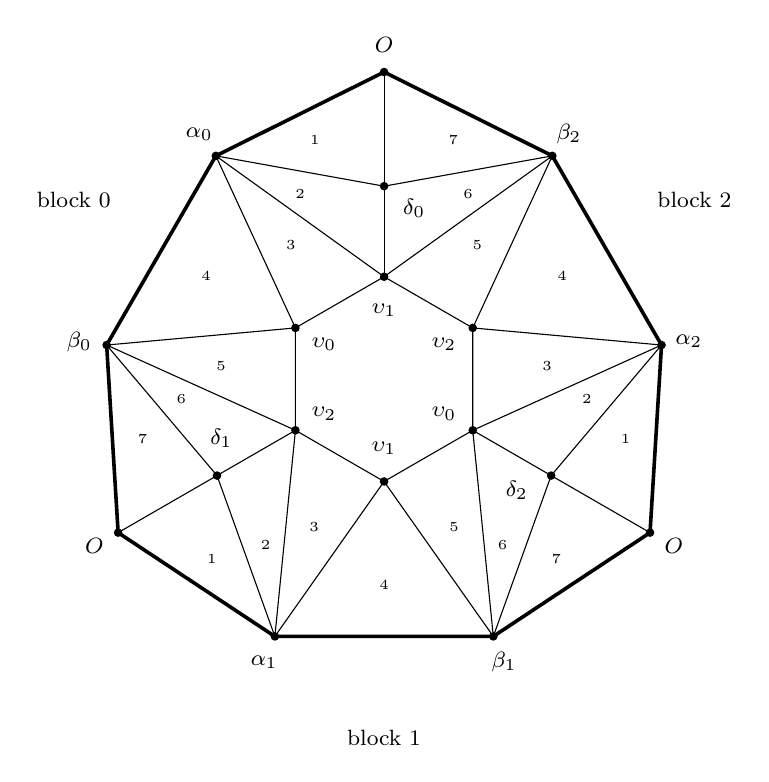
\begin{tikzpicture}[x=1cm,y=1cm,every node/.style={font=\footnotesize},
   dot/.style={circle,fill=black,inner sep=1.1pt},
   lab/.style={fill=white,inner sep=1pt}]
\foreach \i in {0,1,2} {
  \pgfmathsetmacro{\a}{90+120*\i}
  \coordinate (O\i) at (\a:3.9);
  \coordinate (D\i) at (\a:2.45);
  \coordinate (H\i) at (\a:1.3);
  \coordinate (M\i) at (\a+60:1.3);
  \coordinate (A\i) at (\a+37:3.55);
  \coordinate (B\i) at (\a+83:3.55);
}
\foreach \i/\j in {0/1,1/2,2/0} {
  \draw (O\i)--(D\i)--(H\i);
  \draw (D\i)--(A\i)--(H\i)--(M\i)--(A\i);
  \draw (M\i)--(B\i)--(H\j)--(M\i);
  \draw (B\i)--(D\j);
  \draw[line width=1.3pt] (O\i)--(A\i)--(B\i)--(O\j);
  \node at (barycentric cs:O\i=1,D\i=1,A\i=1.4) {\tiny 1};
  \node at (barycentric cs:D\i=1,A\i=2,H\i=1) {\tiny 2};
  \node at (barycentric cs:A\i=1.3,H\i=1,M\i=1) {\tiny 3};
  \node at (barycentric cs:A\i=1,M\i=1,B\i=1) {\tiny 4};
  \node at (barycentric cs:B\i=1.3,M\i=1,H\j=1) {\tiny 5};
  \node at (barycentric cs:B\i=2,H\j=1,D\j=1) {\tiny 6};
  \node at (barycentric cs:B\i=1.4,D\j=1,O\j=1) {\tiny 7};
}
\foreach \i/\j in {0/1,1/2,2/0} {
  \pgfmathsetmacro{\a}{90+120*\i}
  \foreach \p in {O\i,D\i,H\i,M\i,A\i,B\i} \node[dot] at (\p) {};
  \node at (\a:4.25) {$O$};
  \node at (\a+37:3.9) {$\alpha_{\i}$};
  \node at (\a+83:3.9) {$\beta_{\i}$};
  \node[lab] at (\a-10:2.2) {$\delta_{\i}$};
  \node at (\a:0.88) {$\upsilon_{\j}$};
  \node at (\a+60:0.88) {$\upsilon_{\i}$};
  \node at (\a+60:4.55) {block $\i$};
}
\end{tikzpicture}
\caption{The $21$ triangles, drawn as an annulus of three blocks; the numbers $1,\ldots,7$ are those of the triangles within their block. The outer boundary (bold) consists of the three loops $\ell_0,\ell_1,\ell_2$, and its three corners marked $O$ are the same vertex of $\Delta$. The inner hexagon is not a boundary: opposite vertices of the hexagon carry the same label, and opposite edges are the same edge of $\Delta$. Hence every edge that is not bold lies in exactly two of the triangles.}
\label{fig:triangles}
\end{figure}

\emph{The circle space $Z$ and its orbit filling.} The space $Z$ is built from the following pieces.
\begin{itemize}
\item \emph{Six copies of $\mathbb T\times\Delta$,} one for each basis $b\in\{1,\ldots,6\}$. The circle group $\mathbb T$ acts freely on each copy by translation in the first coordinate $t\in\mathbb T$.
\item \emph{Nine cylinders $\mathbb T^2\times[0,1]$,} one for each edge $e=ik$ of $K_{3,3}$ (with $i\le3<k$).
\item \emph{Attachments.} For an end $b\in\{i,k\}$ of $e$, let $r(b,e)\in\mathbb Z/3$ be the index of the loop that corresponds to the plane $P_e$ at basis $b$: if $A_{b,e}$ is $A_q$ or $A_q^c$ with $q\in\{1,2,3\}$, then $r(b,e)=q-1$, which is the index of position $q$ among the tail positions. In particular $r(3,36)=r(6,36)=2$. The point $(t,u,0)$ of the cylinder of $e$ is attached to the point $(t,\ell_{r(i,e)}(u))$ of copy $i$. The point $(t,u,1)$ is attached to the point $(t,\ell_{r(k,e)}(u))$ of copy $k$ if $e\ne36$, and to the point $(t+u,\ell_2(-u))$ of copy $6$ if $e=36$.
\end{itemize}
Thus each cylinder joins the torus $\{(t,\ell_{r(i,e)}(u)):t,u\in\mathbb T\}$ in copy $i$ to the torus $\{(t,\ell_{r(k,e)}(u)):t,u\in\mathbb T\}$ in copy $k$. Every attaching map commutes with translation in $t$. Hence the resulting compact polyhedron $Z$ carries a free $\mathbb T$-action and is a circle space, with half-turn $t\mapsto t+3/2$. Its quotient $Z/\mathbb T$ consists of six copies of $\Delta$ connected along nine cylinders over loops, and it is connected because $\Delta$ is connected.

Write $o\in H_1(Z;\Ftwo)$ for the homology class of a single $\mathbb T$-orbit; because $Z/\mathbb T$ is connected, transporting along a path shows that all orbits represent the same class $o$. For each basis $b\in\{1,\ldots,6\}$ and $m\in\mathbb Z/3$, let $s_{bm}\in H_1(Z;\Ftwo)$ be the class of the loop $u\mapsto(0,\ell_m(u))$ in copy $b$. By the $21$-triangle homology inside $\Delta$,
\[
 \sum_{m\in\mathbb Z/3} s_{bm}=0\qquad\text{for every }b\in\{1,\ldots,6\}.
\]
Across the cylinder of each of the eight uncomplemented edges, the two matched loops $s_{i,r(i,e)}$ and $s_{k,r(k,e)}$ are homotopic and therefore equal in $H_1(Z;\Ftwo)$. Across the cylinder of the complemented edge $36$ of $K_{3,3}$, the loop $u\mapsto(0,\ell_2(u))$ in basis $3$ is homotopic to $u\mapsto(u,\ell_2(-u))$ in basis $6$, whose homology class in the end torus $\mathbb T\times\ell_2(\mathbb T)$ is $o+s_{6,2}$ (both coordinate degrees are odd mod $2$). Thus $s_{3,2}+s_{6,2}=o$. Summing the six chart relations $\sum_m s_{bm}=0$ over all $b=1,\ldots,6$ pairs up all eighteen classes along the nine edges of $K_{3,3}$, yielding $o=0$ in $H_1(Z;\Ftwo)$. Consequently, choosing a point $x_0$ on the orbit of $(0,O)$ in one copy, there exists a singular $2$-chain $x_1\in C_2(Z;\Ftwo)$ with $\partial x_1=Bx_0$.

\emph{Equivariant map $Z\to\B(F_{\rm phys})$.} At any point $(t,p)\in\mathbb T\times\Delta$ in copy $b$, define a pair of probability measures $(\mu_{b,t,p},\nu_{b,t,p})$ on the words of basis $b$ in~\eqref{eq:finite-words} as the laws of the rounded word
\[
 \omega(s,p)=\bigl(\lfloor s\rfloor,\;\lfloor s+p_0\rfloor,\;\lfloor s+p_1\rfloor,\;\lfloor s+p_2\rfloor\bigr)\pmod3
\]
when $s$ is drawn uniformly from $[t,t+1/2]$ (for $\mu_{b,t,p}$) and uniformly from $[t+3/2,t+2]$ (for $\nu_{b,t,p}$), pushing each word forward to its projective measurement in $V(F_{\rm phys})$. Writing $s=\lfloor s\rfloor+\{s\}$, rounding the coordinates of $p+\{s\}\mathbf 1$ always selects a vertex of the minimal ordered simplex of $\mathbb T^3$ containing $p$, which lies in $\Delta$ because $p\in\Delta$; hence $\omega(s,p)$ always belongs to the $39$ retained words~\eqref{eq:finite-words}.

Any word in $\operatorname{supp}\mu_{b,t,p}$ occurs on a set of positive measure in $(t,t+1/2)$, and any word in $\operatorname{supp}\nu_{b,t,p}$ occurs on a set of positive measure in $(t+3/2,t+2)$. For every $s\in(t,t+1/2)$ and $s'\in(t+3/2,t+2)$, the difference $s'-s$ lies strictly in $(1,2)$, so $\lfloor s'+c\rfloor-\lfloor s+c\rfloor\in\{1,2\}$ for every real $c$, hence $\lfloor s+c\rfloor\not\equiv\lfloor s'+c\rfloor\pmod3$. Thus every word in $\operatorname{supp}\mu_{b,t,p}$ differs from every word in $\operatorname{supp}\nu_{b,t,p}$ in all four positions, making their measurements orthogonal at every color and hence adjacent in $F_{\rm phys}$. Writing $s=t+a$ ($a\in[0,1/2]$), the rounding thresholds in $a$ form a finite set of measure zero for every $(t,p)$, so bounded convergence ensures continuity in $(t,p)$. Shifting $t$ by $3/2$ (the half-turn on $Z$) exchanges the intervals $[t,t+1/2]$ and $[t+3/2,t+2]$, hence exchanges the two shores.

Finally, on a matched loop $p=\ell_i(u)=u\alpha_i$, the sampled word $\omega(s,\ell_i(u))$ takes color $\lfloor s\rfloor\pmod3$ on position $0$ and on the tail position indexed by $i$, and color $\lfloor s+u\rfloor\pmod3$ on the other two positions. At every end of a cylinder other than the basis-$6$ end of the complemented edge $36$ of $K_{3,3}$, the former two positions form the set $A_{b,e}$ of plane positions, so the word returns $\lfloor s\rfloor$ on $P_e$ and $\lfloor s+u\rfloor$ on $I-P_e$. At the basis-$6$ end of edge $36$ they form the complement of $A_{6,36}$; there the attaching map replaces $(s,u)$ by $(s+u,-u)$, which turns $(\lfloor s\rfloor,\lfloor s+u\rfloor)$ into $(\lfloor s+u\rfloor,\lfloor s\rfloor)$, so that the word again returns $\lfloor s\rfloor$ on $P_{36}$ and $\lfloor s+u\rfloor$ on $I-P_{36}$. Because the chart maps agree identically on the two ends of every cylinder, extending them constantly along the cylinder parameter $[0,1]$ defines a continuous equivariant map $Z\to\B(F_{\rm phys})$. Together with $(x_0,x_1)$, this forms a tower of length one over $F_{\rm phys}$.

\section{Random descents: the upper bound on the sparse family}\label{app:readings}

This appendix proves the two propositions behind Corollary~\ref{cor:linear-growth}. Both color the sparse graphs with few colors by composing random maps that send each level of the iteration to the preceding one. Such a map exists once one edge of $K_{3,3}$ is exempted from the parity condition of Lemma~\ref{lem:parity}; the price is that a few vertices near the exempted edge must be left out.

\subsection{Choices of positions with one defective edge}\label{app:defect}

A \emph{choice of positions} is a map $\sigma:\{1,\ldots,6\}\to\{0,1,2,3\}$, as in Lemma~\ref{lem:parity}. Let $e=ik$ be an edge of $K_{3,3}$ and let $b\in\{i,k\}$ be one of its ends. A pair $(x,y)$ in the endpoint layer of the wire along $e$ at $b$ is the word of basis chart $b$ that takes $x$ on $A_{b,e}$ and $y$ on $A_{b,e}^c$, so its entry at position $\sigma(b)$ is $x$ if $\sigma(b)\in A_{b,e}$ and $y$ otherwise. Accordingly, we say that $\sigma$ \emph{points to the first entry} at the end $b$ of $e$ if $\sigma(b)\in A_{b,e}$, and that it \emph{points to the second entry} there otherwise. The edge $e$ is \emph{consistent} for $\sigma$ if $\sigma$ points to the same entry at both ends of $e$, and \emph{defective} otherwise. In these terms, Lemma~\ref{lem:parity} says that every choice of positions has a defective edge.

\begin{lemma}\label{lem:one-defect}
For every edge $e_0$ of $K_{3,3}$ there are exactly sixteen choices of positions whose only defective edge is $e_0$. If $\sigma$ is drawn uniformly from these sixteen, then for every edge $e$ of $K_{3,3}$ and each end $b$ of $e$, it points to the first entry at the end $b$ of $e$ with probability $1/2$.
\end{lemma}
\begin{proof}
For a basis $b$ and $r\in\{1,2,3\}$, let $\beta_r(b)\in\Ftwo$ be $1$ if $\sigma(b)\in A_r$ and $0$ otherwise. The triple $(\beta_1(b),\beta_2(b),\beta_3(b))$ equals $(1,1,1)$ if $\sigma(b)=0$ and has its single $1$ in place $\sigma(b)$ otherwise. Thus the four positions correspond bijectively to the four triples with $\beta_1(b)+\beta_2(b)+\beta_3(b)=1$.

By Table~\ref{tab:edges}, each of the eighteen pairs $(b,r)$ belongs to exactly one edge: for $e=ik$ with $i\le3<k$ there are unique $r,r'$ with $A_{i,e}=A_r$ and $A_{k,e}\in\{A_{r'},A_{r'}^c\}$, and the complement occurs only for $e=36$. Write $z_e=\beta_r(i)$ and $z'_e=\beta_{r'}(k)$, and put $c_e=0$ for $e\ne36$ and $c_{36}=1$. Then $\sigma$ points to the first entry at the row end of $e$ exactly when $z_e=1$, and at the column end exactly when $z'_e+c_e=1$. Hence $e$ is consistent when $z'_e=z_e+c_e$ and defective when $z'_e=z_e+c_e+1$.

Fix $e_0$, and put $\hat c_e=c_e$ for $e\ne e_0$ and $\hat c_{e_0}=c_{e_0}+1$. A choice of positions whose only defective edge is $e_0$ is the same as a vector $(z_e)\in\Ftwo^9$, with $z'_e=z_e+\hat c_e$, such that the three bits at every basis sum to $1$:
\[
 \sum_{e\ni i}z_e=1\quad(i\le3),\qquad
 \sum_{e\ni k}z_e=1+\sum_{e\ni k}\hat c_e\quad(k\ge4).
\]
The left-hand sides are given by the vertex--edge incidence matrix of $K_{3,3}$. Because $K_{3,3}$ is connected, the only linear relation among the six rows of this matrix over $\Ftwo$ is that they sum to zero. The six right-hand sides sum to $6+\sum_e\hat c_e=c_{36}+1=0$, so the system is solvable, and its solutions form a coset of the kernel, which has dimension $9-5=4$. This gives sixteen choices.

Let $C$ be a four-cycle of $K_{3,3}$. Adding $1$ to $z_e$ for the four edges $e$ of $C$ changes every left-hand side by $0$ or $2$, so it maps solutions to solutions, and it changes $z_e$ and $z'_e$ for every $e\in C$. Every edge of $K_{3,3}$ lies on a four-cycle. Hence, for a uniformly random solution, each bit $z_e$ and each bit $z'_e$ is uniformly distributed. The entry to which $\sigma$ points at an end of $e$ is determined by $z_e$ or by $z'_e$, which proves the last assertion.
\end{proof}

\subsection{Descents when the wires have interior layers}\label{app:descent-interior}

Let $\lambda\ge1$ and let $H$ be a finite graph. A \emph{cut} $(e_0,\sigma,\ell_0)$ consists of an edge $e_0$ of $K_{3,3}$, a choice of positions $\sigma$ whose only defective edge is $e_0$, and an interior layer $\ell_0\in\{1,\ldots,\lambda\}$. Its \emph{descent map} $\rho$ is defined on all vertices of $S_\lambda(H)$ outside layer $\ell_0$ of the wire along $e_0$ and takes values in $V(H)$:
\begin{itemize}
\item a word $g$ of basis chart $b$ is sent to its entry $g_{\sigma(b)}$;
\item an interior vertex $(e,\ell,x,y)$ with $e=ik$ is sent to $x$ if $\sigma$ points to the first entry at the end of $e$ assigned to the layer $\ell$, and to $y$ otherwise. The end assigned to $\ell$ is $i$ if $e=e_0$ and $\ell<\ell_0$, and $k$ if $e=e_0$ and $\ell>\ell_0$; if $e\ne e_0$, either end may be taken, since $\sigma$ points to the same entry at both.
\end{itemize}
By the definition of pointing to an entry, the first rule sends a pair $(x,y)$ in an endpoint layer of the wire along $e$ at $b$ to $x$ if $\sigma$ points to the first entry at the end $b$ of $e$, and to $y$ otherwise. In this sense the second rule extends to the endpoint layers, with the end $b$ assigned to the endpoint layer at $b$.

A cut is \emph{uniformly random} if $e_0$ is uniform among the nine edges, $\sigma$ is uniform among the sixteen choices of Lemma~\ref{lem:one-defect} for $e_0$, and $\ell_0$ is uniform among the $\lambda$ interior layers and independent of $\sigma$.

\begin{lemma}\label{lem:reading-hom}
The descent map of a cut is a graph homomorphism from the subgraph of $S_\lambda(H)$ induced on its domain to $H$. For a uniformly random cut, an interior vertex $(e,\ell,x,y)$ lies outside the domain with probability $\delta=1/(9\lambda)$ and, conditionally on lying inside, is sent to $x$ with probability $1/2$ and to $y$ with probability $1/2$. Words of basis charts always lie in the domain.
\end{lemma}
\begin{proof}
Let $u,v$ be adjacent vertices in the domain. If they are words of the same basis chart $b$, their entries at $\sigma(b)$ are adjacent in $H$. Otherwise they are pairs $(x,y)$ and $(x',y')$ in equal or consecutive layers $\ell,\ell'$ of one wire, with $x\sim_Hx'$ and $y\sim_Hy'$. If this wire is not the one along $e_0$, then $u$ and $v$ are both sent to their first entries or both to their second entries. If it is the wire along $e_0$, the layers $\ell$ and $\ell'$ are different from $\ell_0$ and differ from each other by at most one, so they lie on the same side of $\ell_0$ and are assigned the same end; again $u$ and $v$ are both sent to their first entries or both to their second entries. In each case the images are adjacent in $H$.

The vertex $(e,\ell,x,y)$ lies outside the domain exactly when $e_0=e$ and $\ell_0=\ell$, which has probability $1/(9\lambda)$. Once $e_0$ and $\ell_0$ are given, the end assigned to the layer $\ell$ is determined, and by Lemma~\ref{lem:one-defect} the random $\sigma$ points to the first entry there with probability $1/2$.
\end{proof}

Now apply this at every level of the iteration. For $h\ge1$ choose a uniformly random cut for $S_\lambda(H)$ with $H=S^{m-1}_\lambda(K_3)$ at each level $m=1,\ldots,h$, independently, and let $\kappa_h$ be the composition of the $h$ descent maps; put $\kappa_0=\mathrm{id}$. Thus $\kappa_h$ is a random map from a subset of $V(S^h_\lambda(K_3))$, its \emph{domain}, to the three colors, and by Lemma~\ref{lem:reading-hom} it is a proper $3$-coloring of the subgraph induced on its domain.

\begin{lemma}\label{lem:reading-failure}
Let $\lambda\ge1$ and $p_*=2/(9\lambda+1)$. Every vertex of $S^h_\lambda(K_3)$ that admits a presentation lies outside the domain of $\kappa_h$ with probability at most $p_*$. A padded scalar always lies in the domain.
\end{lemma}
\begin{proof}
We argue by induction on $h$; for $h=0$ there is nothing to prove. Let $h\ge1$. A padded scalar at level $h$ is the constant word of basis $6$ on the same scalar padded to level $h-1$. It is a word of a basis chart, so it lies in the domain of the descent map at level $h$, which sends it to that padded scalar; by induction it lies in the domain of $\kappa_h$.

Let $v$ be a vertex with a presentation whose root is an internal node. If the root is a basis node, or a wire node whose layer is $0$ or $\lambda+1$, then $v$ is a word of a basis chart, and its entries are the values of the children of the root. The descent map at level $h$ sends $v$ to one of these entries, chosen by the cut at level $h$. Each entry admits a presentation, namely a subtree, and the cuts at lower levels are independent of the cut at level $h$. By induction, $v$ lies outside the domain of $\kappa_h$ with probability at most $p_*$.

If the root is a wire node with an interior layer, its children have values $x$ and $y$, where the background $y$ is a padded scalar. By Lemma~\ref{lem:reading-hom}, $v$ lies outside the domain of the descent map at level $h$ with probability $\delta$, and otherwise it is sent to $x$ or to $y$ with probability $1/2$ each, independently of the lower levels. The padded scalar $y$ always lies in the domain of $\kappa_{h-1}$, and $x$ lies outside it with probability at most $p_*$ by induction. Hence $v$ lies outside the domain of $\kappa_h$ with probability at most
\[
 \delta+(1-\delta)\,\frac{p_*}{2}
 =\frac{1}{9\lambda}+\frac{9\lambda-1}{9\lambda}\cdot\frac{1}{9\lambda+1}
 =\frac{2}{9\lambda+1}=p_* .\qedhere
\]
\end{proof}

\begin{proposition}\label{prop:readings}
Let $\lambda\ge1$ and $h\ge0$, and let $F$ be a subgraph of $S^h_\lambda(K_3)$ each of whose vertices admits a presentation. If $\chi(F)\ge t$, then
\[
 |V(F)|\ge\Bigl(\frac{9\lambda+1}{2}\Bigr)^{\lfloor(t-1)/3\rfloor}.
\]
\end{proposition}
\begin{proof}
Put $q=\lfloor(t-1)/3\rfloor$ and take $q$ independent copies $\kappa^{(1)},\ldots,\kappa^{(q)}$ of $\kappa_h$. By Lemma~\ref{lem:reading-failure}, the expected number of vertices of $F$ that lie in none of the $q$ domains is at most $|V(F)|\,p_*^q$. If this number were less than $1$, some outcome would have every vertex of $F$ in at least one domain. Color each vertex $v$ of $F$ by the pair $(m,\kappa^{(m)}(v))$, where $m$ is the least index with $v$ in the domain of $\kappa^{(m)}$. Two adjacent vertices with the same index $m$ receive different colors, because $\kappa^{(m)}$ is a proper coloring of the subgraph of $S^h_\lambda(K_3)$ induced on its domain. This would be a proper coloring of $F$ with $3q\le t-1$ colors. Hence $|V(F)|\ge p_*^{-q}$.
\end{proof}

\subsection{Descents without interior layers}\label{app:descent-zero}

Let $\lambda=0$. Then every vertex of $S_0(H)$ is a word of a basis chart, and the edges along the wire of $e=ik$ join the pairs $(x,y)$ at the end $i$ to the pairs $(x',y')$ at the end $k$ with $x\sim_Hx'$ and $y\sim_Hy'$. A word of basis chart $b$ is \emph{two-valued along $e$}, for an edge $e$ at $b$, if it takes one value on $A_{b,e}$ and a different value on $A_{b,e}^c$. A word that takes exactly two values, each at two positions, takes one value on $A_r$ and the other on $A_r^c$ for the unique $r$ with $g_r=g_0$; by Table~\ref{tab:edges} it is therefore two-valued along exactly one edge at its basis.

A \emph{cut} $(e_0,\sigma,b_0)$ now consists of an edge $e_0$ of $K_{3,3}$, a choice of positions $\sigma$ whose only defective edge is $e_0$, and an end $b_0$ of $e_0$. Its \emph{descent map} $\rho$ sends a word $g$ of basis chart $b$ to its entry $g_{\sigma(b)}$ and is defined on all words except those of basis chart $b_0$ that are two-valued along $e_0$. The cut is \emph{uniformly random} if $e_0$ is uniform among the nine edges, $\sigma$ is uniform among the sixteen choices of Lemma~\ref{lem:one-defect} for $e_0$, and $b_0$ is uniform among the two ends of $e_0$ and independent of $\sigma$.

\begin{lemma}\label{lem:zero-reading}
For $\lambda=0$, the descent map of a cut is a graph homomorphism from the subgraph of $S_0(H)$ induced on its domain to $H$. For a uniformly random cut, a word that takes exactly two values, each at two positions, lies outside the domain with probability $1/18$ and, conditionally on lying inside, is sent to each of its two values with probability $1/2$. All other words always lie in the domain.
\end{lemma}
\begin{proof}
Let $u,v$ be adjacent words in the domain. If they belong to the same basis chart $b$, their entries at $\sigma(b)$ are adjacent in $H$. Otherwise they are pairs $(x,y)$ and $(x',y')$ at the two ends of one wire, along an edge $e$, with $x\sim_Hx'$ and $y\sim_Hy'$. If $e\ne e_0$, then $\sigma$ points to the same entry at both ends, so the images are $x,x'$ or $y,y'$. If $e=e_0$, say with $u$ at the end $b_0$, then $u$ is not two-valued along $e_0$, so $x=y$; its image $x$ is adjacent to both $x'$ and $y'$, one of which is the image of $v$.

A word that takes exactly two values, each at two positions, is two-valued along exactly one edge $e$ at its basis $b$. It lies outside the domain exactly when $(e_0,b_0)=(e,b)$, which has probability $1/18$. Once $e_0$ and $b_0$ are given, whether it lies in the domain is determined, and by Lemma~\ref{lem:one-defect} the random $\sigma$ points to the first entry at the end $b$ of $e$ with probability $1/2$. A word of any other kind is not two-valued along any edge.
\end{proof}

As before, compose the descent maps of independent uniformly random cuts at the levels $1,\ldots,h$ to obtain a random map $\kappa_h$ from a subset of $V(S^h_0(K_3))$ to the three colors. It is a proper $3$-coloring of the subgraph induced on its domain.

\begin{lemma}\label{lem:zero-success}
Let $\lambda=0$ and $\beta=\log_2(18/17)$. A vertex of $S^h_0(K_3)$ that has a presentation with $L$ leaves lies in the domain of $\kappa_h$ with probability at least $L^{-\beta}$.
\end{lemma}
\begin{proof}
We argue by induction on $h$; for $h=0$ the probability is $1$. Let $h\ge1$ and fix a presentation of $v$ with $L$ leaves. Because $\lambda=0$, every wire node has layer $0$ or $1$, so $v$ is a word of a basis chart. If the presentation is a single leaf, $v$ is a constant word whose entries are the same scalar padded to level $h-1$; otherwise the entries of $v$ are the values of the children of the root.

Suppose first that $v$ takes exactly two values $x\ne y$, each at two positions. By Lemma~\ref{lem:zero-reading}, $v$ lies in the domain of the descent map at level $h$ with probability $17/18$ and is then sent to $x$ or to $y$ with probability $1/2$ each, independently of the lower levels. The values $x$ and $y$ are the values of two different children of the root; let $L_x$ and $L_y$ be the numbers of leaves of their subtrees, so that $L_x+L_y\le L$. By induction, by the convexity of $s\mapsto s^{-\beta}$, and because $2^\beta=18/17$, the vertex $v$ lies in the domain of $\kappa_h$ with probability at least
\[
 \frac{17}{18}\cdot\frac{L_x^{-\beta}+L_y^{-\beta}}{2}
 \ \ge\ \frac{17}{18}\Bigl(\frac{L_x+L_y}{2}\Bigr)^{-\beta}
 \ \ge\ \frac{17}{18}\,2^\beta L^{-\beta}=L^{-\beta}.
\]
In every other case $v$ lies in the domain of the descent map at level $h$, which sends it to one of its entries. That entry has a presentation with at most $L$ leaves, so by induction it lies in the domain of $\kappa_{h-1}$ with probability at least $L^{-\beta}$.
\end{proof}

\begin{proposition}\label{prop:zero-layer}
Let $\beta=\log_2(18/17)$. For every $j\ge1$, the graphs $G_{j,1}$ and $G_{j,2}$ coincide and satisfy $\chi(G_{j,1})=O(j^{1+\beta})$, with an absolute implicit constant.
\end{proposition}
\begin{proof}
Both graphs are defined with $\lambda=0$, so they coincide and are induced subgraphs of $S^j_0(K_3)$. Every vertex has a presentation with at most $2j-1$ internal nodes, each with at most three children, hence with at most $1+2(2j-1)=4j-1$ leaves. By Lemma~\ref{lem:zero-success} it lies in the domain of $\kappa_j$ with probability at least $p=(4j-1)^{-\beta}$. Write $n=|V(G_{j,1})|$ and take $k=\lceil(1+\log n)/p\rceil$ independent copies of $\kappa_j$. The expected number of vertices that lie in none of the $k$ domains is at most $n(1-p)^k\le n\,e^{-pk}<1$, so some outcome has every vertex in at least one domain. Coloring each vertex by the least index of a domain containing it and by its color there is a proper coloring with $3k$ colors, as in the proof of Proposition~\ref{prop:readings}. Theorem~\ref{thm:sparse} gives $\log n=O(j)$, so $3k=O(j^{1+\beta})$.
\end{proof}


\bibliographystyle{unsrtnat}
\bibliography{references}

\end{document}
